\documentclass[12pt]{report}
\usepackage{epsfig}
\usepackage{epstopdf}





\renewcommand{\baselinestretch}{1}
\pagestyle{headings}
\setcounter{page}{1}
\usepackage[left=1.5in, right=1.0in, top=1.0in, bottom=1.0in]{geometry}
\usepackage{layout}
\usepackage{setspace}
\usepackage{aeguill}
\usepackage{lscape }
\newcommand{\stereotype}[1]{
	\guillemotleft {#1}\guillemotright
}

%\usepackage{rotfloat }
%\usepackage{sidewaystable}
\doublespacing
\usepackage{amsmath}
\usepackage{amsthm}
\usepackage{dsfont}
\usepackage{cuthesis}
%\usepackage{stmaryrd}
\usepackage{epsfig}
\usepackage{amsfonts}
\usepackage{multirow}
\usepackage{alltt}
\usepackage{framed}
%%packages
%\usepackage{amsmath}
%\usepackage{setspace}
\usepackage{subfig}
%\usepackage[mathscr]{euscript}
\usepackage{mathrsfs}
%\usepackage{pst-node}
%\usepackage{dsfont} % for mathds
%\usepackage{helvet}
%\usepackage{courier}
\usepackage{gastex}
%%\usepackage{ps4pdf}
%%\PSforPDF{usepackage{pst-all}}
%%\usetheme{Warsaw}
\usepackage{graphicx}
\usepackage[graphicx]{realboxes}
%\usepackage{makeidx}
%\usepackage{makeidx}
%\usepackage{multicol}
%\usepackage{footmisc}
%\usepackage{times}
\usepackage{graphics}
%\usepackage{epsfig}
%\usepackage{amsthm}
\usepackage{mathptmx}
%\usepackage[ruled,vlined]{algorithm2e}
\usepackage[psamsfonts]{amssymb} % needed for \rightarrowtail
\usepackage[only,varotimes,varodot]{stmaryrd} % needed for \varotimes
\usepackage{mathtools} % in order to use Coloneqq
%\usepackage{array}
\usepackage{bussproofs} % for proofs
%\usepackage{dsfont}
%\usepackage{gastex}
%\usepackage{alltt}
%\usepackage{hyperref}
%\usepackage{wrapfig}
%\usepackage[babel=true]{csquotes}
%%\usepackage[french]{babel}
%
\usepackage{fancybox} % used for shadow box
%\usepackage{multirow}
%\usepackage{longtable}
\usepackage{listings}
%\usepackage{pdflscape} %landscape package
%
%%\usepackage{MnSymbol}
\usepackage{algorithm}
%\usepackage{algorithmic}
% %Define code packages and options pseudocode
\usepackage{algorithmicx}
\usepackage{algpseudocode}
%%\algrenewcommand{\algorithmiccomment}[1]{\\\hskip3em$/*$ #1 $*/$}
%%\algrenewcommand{\Call}[2]{\textit{\mbox{#1}}(#2)}
 \newcommand{\qinput}{\textbf{Input:$~~~~$}}
\newcommand{\qoutput}{\\\textbf{Output: }}
 \newcommand{\sem}[1]{[\![#1]\!]} %semantic
%
%% ----------------------------------------------------------------
%\vfuzz2pt % Don't report over-full v-boxes if over-edge is small
%\hfuzz2pt % Don't report over-full h-boxes if over-edge is small
%% THEOREMS -------------------------------------------------------
\newtheorem{theorem}{Theorem}[chapter]
\newtheorem{corllary}{Corollary}[chapter]
\newtheorem{lemma}{Lemma}[chapter]
\newtheorem{proposition}{Proposition}[chapter]
\newtheorem{property}{Property}[chapter]
\theoremstyle{definition}
%\newtheorem{definition}{Definition}

\newtheorem{remark}{Remark}[chapter]
\newtheorem{axiom}{Axiom}[chapter]
\newtheorem*{theorem*}{Theorem}
\newtheorem*{corollary*}{Corollary}

\newtheorem{definition}{Definition}[chapter]
%\newtheorem{theorem}{Theorem}[chapter]
%\newtheorem{lemma}{Lemma}
%\newtheorem*{proof}{Proof}[section]
%\newtheorem{definition}{Definition}
%\newtheorem{theorem}{Theorem}
%\newproof{proof}{Proof}

%\numberwithin{equation}{section}
% MATH -----------------------------------------------------------
\newcommand{\norm}[1]{\left\Vert#1\right\Vert}
\newcommand{\abs}[1]{\left\vert#1\right\vert}
\newcommand{\set}[1]{\left\{#1\right\}}
\newcommand{\Real}{\mathbb R}
\newcommand{\eps}{\varepsilon}
\newcommand{\To}{\longrightarrow}
\newcommand{\BX}{\mathbf{B}(X)}
\newcommand{\A}{\mathcal{A}}

%Macro


\newcommand{\nmarked}[2]{{\overline{#1}}^{#2}} % marking #1 by the #2 number of tokens
\newcommand{\marked}[1]{\overline{#1}} %marking #1 by one overbar

\newcommand{\activityedge}{\!\rightarrowtail\!}
\newcommand{\labeled}[2]{#1\colon\!#2}
\newcommand{\emptyaction}{o}

\newcommand{\ie}{i.e.~\/}
\newcommand{\eg}{e.g.~\/}
\newcommand{\etc}{etc.\/}

\newcommand{\con}[1]{{\sf #1}}
\newcommand{\ty}[1]{\mbox{\sl #1}}
\newcommand{\ml}[1]{\mbox{\tt #1}}
\newcommand{\ma}[1]{{{$#1$}}}
\newcommand{\prev}[1]{#1}
\newcommand\fun{{\to}}
%\renewcommand{\prod}{\times}
\newcommand\imp{{\Rightarrow}}
\newcommand\T{\con{T}}
\newcommand\F{\con{F}}
\newcommand\qq{\mbox{\tt{`\hspace{-1.0mm}`}}}
\newcommand\termbddty{\ty{termbdd}}
\newcommand{\termbdd}[3]{\mbox{$#1~#2~\mapsto~#3$}}
\newcommand{\globtermbdd}[2]{\mbox{$#1\hspace{0.5mm}\mapsto\hspace{0.5mm}#2$}}
\newcommand{\BOX}{\hfill $\Box$}




\newcommand{\algoWithLineNumbers}[3]{{
  \begin{algorithm}
  \caption[#1]{\sc #1}
  \label{#2}
  \begin{algorithmic}[1]
    #3
  \end{algorithmic}
  \end{algorithm}}} \newcommand{\algo}[3]{{
  \begin{algorithm}
  \caption[#1]{\sc #1}
  \label{#2}
  \begin{algorithmic}
    #3
  \end{algorithmic}
  \end{algorithm}}}
\begin{document}
\cusym{ACL}{Agent Communication Language}
\cusym{AI}{Artificial Intelligence}
\cusym{ARCTL}{Action Restricted Computation Tree Logic}
\cusym{BDD}{Binary Decision Diagram}
\cusym{BNF}{Backus-Naur Form}
\cusym{CTL}{Computation Tree Logic}
\cusym{CTLC}{Computation Tree Logic of Commitment}
\cusym{CTLK}{Computation Tree Logic of Knowledge}
\cusym{CTLKC}{Computation Tree Logic of Knowledge and Commitment}
\cusym{CWB-NC}{Concurrency WorkBench of New Century }
\cusym{DTMC}{Discrete-Time Markov Chain}
\cusym{FIPA}{Foundation for Intelligent Physical Agents}
\cusym{ISPL}{Interpreted Systems Programming Language}
\cusym{KQML}{Knowledge Query and Manipulation Language}
\cusym{LTL}{Linear Temporal Logic}
\cusym{MAS}{Multi-Agent System}
\cusym{MCK}{Model Checking Knowledge}
\cusym{MCMAS}{Model Checker for Multi-Agent Systems}
\cusym{MDP}{Markov Decision Process}
\cusym{NuSMV}{New Symbolic Model Verifier}
\cusym{PCTL}{Probabilistic Computation Tree Logic}
\cusym{PCTLC}{Probabilistic Computation Tree Logic of Commitment}
\cusym{PCTLK}{Probabilistic Computation Tree Logic of Knowledge}
\cusym{PO-DTMC}{Partially Observable Discrete-Time Markov Chain}
\cusym{POMDP}{Partially Observable Markov Decision Process}
\cusym{PRISM}{PRobabilistIc Symbolic Model checker}
\cusym{PSPASE}{Polynomial Space}
\cusym{SMV}{Symbolic Model Verifier}
\cusym{SPIN}{Simple Promela INterpreter}
\cusym{TS}{Transition System}
\cusym{UML}{Unified Modeling Language}

\typeout{------> Cover}
%\cutitle{A Logic-based Framework for Addressing Probabilistic Social Commitments in Multi-Agent Systems}

%\cutitle{Probabilistic Social Commitments in Multi-Agent Systems: Representation and Model Checking}

%\cutitle{On the Probabilistic Social Commitments in Multi-Agent Systems}
%\cutitle{Probabilistic Social Commitments: Representation and Verification}

\cutitle{Dynamic Formation and Strategic Management of Web Services Communities}

\cudept{Computer Science and Software Engineering}   % your dept.
\cudegree{Doctor of Philosophy}           % your expected degree <-,
\cudegreeshort{Ph.~D.}
\culname{Khosrowshahi-Asl}                    % your family name
\cufname{Ehsan}                    % your given name

\cusupervisor{Dr. Jamal Bentahar}        % your Big-Boss complete name
\cucosupervisor{Dr. Hadi Otrok}   % your small big-boss name
\cuexaminerA{Dr. Peter Grogono}
\cuexaminerB{Dr. Ferhat Khendek}
\cuexaminerC{Dr. Joey Paquet}
%\cuexaminerA{}
\cuextexaminer{Dr. Muhammad Younas}     % Another of the previous kind
\cuchair{Dr. TBA (Chair)}           % the boss of your boss

\cumonth{July}                % the month you expected to graduate
\cuyear{2015}                 % and the year.
%\cudedication{\ \\ \\ \\ \\ \\ \\ \\ \\
%\begin{center}{\bf{To My Parents,\\ My Wife and daughter,\\ and My Brothers and Sisters.}} \\
%\end{center}}
\cuabstract{%        \thispagestyle{plain}
%        \newpage
%        \null\vskip0.50in%
%        \begin{center}
%                {\LARGE\bf{ABSTRACT}}
%        \end{center}

 abstract abstract abstract abstract abstract abstract abstract abstract abstract abstract abstract abstract abstract abstract abstract abstract abstract abstract abstract abstract abstract abstract abstract abstract abstract abstract abstract abstract abstract abstract abstract abstract abstract abstract abstract abstract abstract abstract abstract abstract abstract abstract abstract abstract abstract abstract abstract abstract abstract abstract abstract abstract abstract abstract abstract abstract abstract abstract abstract abstract abstract abstract abstract abstract abstract abstract abstract abstract abstract abstract abstract abstract abstract abstract abstract abstract abstract abstract abstract abstract abstract abstract abstract abstract abstract abstract abstract abstract abstract abstract abstract abstract abstract abstract abstract abstract abstract abstract abstract abstract abstract abstract abstract abstract abstract abstract abstract abstract abstract abstract abstract abstract abstract abstract abstract abstract abstract abstract abstract abstract abstract abstract abstract abstract abstract abstract abstract abstract abstract abstract abstract abstract abstract abstract abstract abstract abstract abstract abstract abstract abstract abstract abstract abstract.


 abstract abstract abstract abstract abstract abstract  abstract abstract abstract abstract abstract abstract abstract abstract abstract abstract abstract abstract abstract abstract abstract abstract abstract abstract abstract abstract abstract abstract abstract abstract abstract abstract abstract abstract abstract abstract abstract abstract abstract abstract abstract abstract abstract abstract abstract abstract abstract abstract abstract abstract abstract abstract abstract abstract abstract abstract abstract abstract abstract abstract abstract abstract abstract abstract abstract abstract abstract abstract abstract abstract abstract abstract abstract abstract abstract abstract abstract abstract abstract abstract abstract abstract abstract abstract abstract abstract abstract abstract abstract abstract abstract abstract abstract abstract abstract abstract abstract abstract abstract abstract abstract abstract abstract abstract abstract abstract abstract abstract abstract abstract abstract abstract abstract abstract abstract abstract abstract abstract abstract abstract abstract abstract abstract abstract abstract abstract.
%The experimental results demonstrate the efficiency and scalability of the proposed reduction techniques and show that our work is effective for addressing probabilistic social commitment in MASs.
\\
%\textbf{keywords:}
%Multi-Agent Systems, Agent Communication, Social Commitments, uncertainty, Model Checking.

%\newpage

%\endinput
}
%%
%
%
%
\cuthanks{I would never have been able to finish my dissertation without the guidance of my committee members, help from friends, and support from my family.

I would like to thank my supervisors, Prof. Jamal Bentahar and Prof. Hadi Otrok for giving me the opportunity to work under their supervision. I am very grateful to them for their valuable suggestions and guidance throughout the preparation of this thesis. I learned a lot of valuable lessons which will be useful for me beyond the scope of this thesis, throughout my lifetime.

I would like to thank my examiner committee Professors Peter Grogono, Ferhat Khendek, Joey Paquet and Muhammad Younas for giving me the honor by being in my PhD committee. Their time and effort are greatly appreciated.

I would like thank my colleague Babak Khosravifar who was always willing to help and give his best suggestions. Also, I would like to thank my friends and lab colleagues Omar Marey, Faisal Al-Saqqar and Khalid Sultan for their help and support.

Finally, I am very grateful to my parents for their understanding, encouragement and their endless support.
}

\cumaketitlepage       % title page, not numbered
\cumakesignaturepage   % sign. page, not numbered
\cumakeabstract
%\cumakededication      % To Mom and Dad
\cumakethanks          % Thanks Boss!
\cutocdeep{4}          % how deep you want to go in the toc: 0: reset to 1
\cumaketableofcontents % Gues\cumakelistoffigures   % id.
\cumakelistoftables    % id.
\cumakelistoffigures
\cumakelistofsymbols   % a gook work should have a list of symbols.
\custartbody    % this initialize double-spacing, page-numbering ...

%%% Local Variables:
%%% TeX-master: "thesis"
%%% End:

\typeout{------> Introduction}

%%%%%%%%%%%%%%%%%%%%%%%%%%%%%%%%%%%%%%%%%%%%%%%%%%%%%%%%%%%%%%%%%%%%%%%%%%%%%%%
%% Chapter 1 : Introduction.
%%%%%%%%%%%%%%%%%%%%%%%%%%%%%%%%%%%%%%%%%%%%%%%%%%%%%%%%%%%%%%%%%%%%%%%%%%%%%%%
%\input{chap1/introduction.tex}

\setcounter{chapter}{0}

\chapter{Introduction}\label{sec:intro}
In this chapter, we introduce the context of this research, which is about communities of web services abstracted as autonomous agents. Those agent-based web services use intelligent decision making mechanisms to improve their performance in multi-agent setting. We discuss the motivations of this work and briefly review the literature to identify the problems we aim to solve in this thesis. Moreover, we discuss our objectives and contributions.

\section{Context of Research}\label{sec:motivation}

Over the past years, online services have become part of many
scalable business applications. The increasing reliance on
web-based applications has significantly influenced the way web
services are engineered. Web services provide a set of online software functions accessible at a network address over the web.
The recent developments are shifting web services from passive and
individual components to autonomous and group-based components
where interaction, composition, and cooperation are the key
challenges \cite{ICWS2011-1,SCC2011-1}. The main objective is to
achieve a seamless integration of business processes, applications
and web services. Delivering high quality services considering the
dynamic and unpredictable nature of the Internet is still a very
critical and challenging issue.

Typically, web services are business applications deployed as
autonomous and interoperable agents \cite{Alescio}. In fact, the
W3C consortium defines a web service as ``an abstract notion that
must be implemented by a concrete agent''. However, the web is
stocked with agent-based services that offer similar business
functionalities, which leads to service consumers having
difficulties in choosing the most appropriate agents to interact
with.

The need for highly available and responsive services has called
for grouping and collaborative mechanisms of loosely-coupled web
services, particularly in business settings. The idea of grouping
web services within communities and the way those communities are
engineered so that web services can better collaborate have been
proposed and investigated in
\cite{DBLP:journals/ijebr/MaamarSTBB09,DBLP:journals/internet/BenatallahSD03,Rosario:2008:PQS:1512146.1512290}.
Communities are virtual groups of web services having similar
functionalities \cite{Zeng:2003:QDW:775152.775211,
Paik:2005:TSS:2229263.2230038,Medjahed05adynamic,10.1109/ARES.2008.7},
but probably different non-functional quality attributes, which
form the QoS parameters.
%When communities are used, users send
%their requests to the masters of those communities, which are
%responsible of managing the communities, forwarding the requests
%to the suitable member web services and checking the credentials
%of those members.
Communities aim to provide higher service
availability and performance than what individual web services can
provide.
%The high availability of services and the community
%resilience to failure are guaranteed since web services can
%cooperate and replace each other within the same community and
%since there is no single point of failure in the communities
%architecture.

\section{Motivating Scenario}\label{sec:motexample}

In this section, we present a scenario and demonstrate why there
is need for communities of services. We first propose an example
of a real world scenario, focusing on user experience. There are a
plethora of options available to people in today's society,
including weather forecasting, ticketing services, map services,
local places guides and so on. Most mobile or web applications
cannot independently satisfy users requests and should rely on
different online services. The high competition within the
services industry requires applications to use reliable and high
quality online services.


If the user were to check a web site or run an application on her
mobile device upon having downtime, or having high response delay
or encountering any non-satisfying quality metric, she will
instantly remove the application, which is a huge business concern
for application providers. For example, if a user installs a
ticketing application on her mobile device and the application is
not using high quality service providers, the user would instantly
uninstall the application, which has an extremely negative impact
on the
visibility of the application. %Let us say you search "Montreal
%Weather" on a search engine and you click on a web site which is
%slow because it is using a bad weather web service as source of
%its raw data, the user will leave the web site and try another
%link from search results, which has a bad Search Engine
%Optimization (SEO) effect for the web site, and search engines
%would not show that web site on search results anymore, which is a
%business and revenue loss for the application.
Thus, end user satisfaction is the main goal for competitive
online providers. Communities of web service, by providing
services with higher quality, higher uptime and reliability for
end users, aim to reach this goal. To this end, community
management decisions should capitalize on important QoS parameters
while forming the community and during membership management.


High demand on online services has created a massive business
competition. For example, nowadays users are provided with
multiple choices of web services offering local places information
such as coffees, venues, and shops nearby a geographic position.
It is hard for new web services to find their customers and be
visible for end users amongst hundreds or thousands of other
available services, even if they provide a high quality of
service. Hence, the concept of communities of web services
provides them with the chance of joining a platform with an
established market share and reputation. However, it is crucial
for a community manager to consider many factors when inviting or
accepting new members. For example, if the market share is not big
enough, bringing new web services can cause revenue drop for the
already residing members. This may encourage other web services to
collude, leave, or join other communities, hurting the community
stability. This is an important issue which has not been addressed
previously in the relevant literature. On the other hand, if
communities bound the number of web services to ensure higher
revenue, availability and response time could be negatively
affected if some members encounter problems. This is because
alternative web services for substitution will be limited.  This
has also not been efficiently addressed in the related work.
Consequently, community formation algorithms satisfying some
desirable properties such as community stability and overall
revenue are yet to be defined considering end users, community
managers and service providers.


\section{Motivation and Research Questions}\label{sec:researchquestions}

Web service communities are dynamic by design
\cite{DBLP:journals/ijebr/MaamarSTBB09}. In these communities, web
services are modeled as intelligent autonomous agents, where they
can adopt a strategy maximizing their payoff at any time. A web
service can ask joining a community and has the right to leave it.
Community managers can invite or ask a web service to leave in
order to maximize the community profit. Users can simply stop
sending requests to a web service which is not providing
satisfactory services. Thus, it is important to consider all the
parties involved in the decision making process about the
community formation and management. Most of the recent work on communities of
services are either user-centric and focus on user satisfaction
\cite{Chun02user-centricperformance} or system-centric and focus
on the whole system throughput, performance and utilization. There
are many contributions in distributed, grid, cluster and cloud
services which are system-centric. However, in real world
environments and applications, both users and service providers
are self-interested agents, aiming to maximize their own profit.
In those environments, both parties (users and services) will
collaborate as long as they are getting more benefits and payoff.
Our initial research question is: \emph{How can we model the
community of agent-based services in order to maximize the utility
of involved users, web services and community organizers?[R1]}


In order to address this problem, recently
\cite{DBLP:conf/IEEEscc/LimTMB12,
DBLP:conf/IEEEscc/KhosravifarABT11, 10.1109/TSC.2012.12} proposed
mechanisms to help users and services maximize their gain. A
two-player non-cooperative game between web services and community master (i.e., manager) was introduced in
\cite{DBLP:conf/IEEEscc/KhosravifarABT11}. In
\cite{DBLP:conf/IEEEscc/LimTMB12}, a 3-way satisfaction approach
for selecting web services has been proposed. In this approach,
the authors proposed a web service selection process that the
community masters can use. The approach considers the efficiency
of all the three involved parties, namely users, web services and
communities. The issue with these solution concepts is that they
consider community as a whole and model it as one entity in their
formulations. A community master decides on behalf of all the
members using an aggregated function of parameters. This can hurt
the overall revenue for some individual web services, or even a
subset of web services. Those services can collude and form their
own community to increase their payoff, instead of having to adjust and share
their resources with other members. Another important issue which
needs to be considered is the community stability. In community of
web services, the members and community organizers collaborate to
perform tasks. Having jointly completed a task and generated
revenue, they need to agree on some reasonable method of dividing
profits (or tasks) among themselves. This is a key issue for the
group stability still to be investigated. If the revenue sharing
mechanism is not fair enough for any subset of web services
working in the community, these agents, as profit maximizing
entities, would deviate and make their own group. Thus, an important an
important research question that we would like to address is:
\emph{How can we model fair and stable communities as coalitions
of agent-based web services?[R2]}

%The consideration of those inputs is a significant
%issue as existing web services can lose utility or payoff because
%of the new member, which can results in an unhealthy and unstable
%group. The problem comes from the fact that the existing members
%should collaborate with the new web services, so probably their
%performance as a group can suffer. Existing members may even
%deviate and try to join other communities if they are unsatisfied.
%Those considerations of forming stable and efficient coalitions
%are the main contributions of our paper.

%However, a high
%performing web service could deviate anytime it finds itself
%unsatisfied within the community instead of adjusting its service
%parameters.


In \cite{10.1109/TSC.2012.12}, a cooperative scheme among
autonomous web services based on coalitional game theory has been
introduced. The authors have proposed an algorithm to reach
individually stable coalition partition for web services in order
to maximize their efficiency. The communities choose new web
services on the promise that it would benefit the community
without decreasing any other web service's income. In their model,
the worth of community is evaluated with high emphasis on the
availability metric and considering price and cost values only.
The community structure is based on a coordination chain, where a
web service is assigned as a \emph{primary} web service and the
community task distribution method will initially invoke the
primary web service. Only if the primary web service is
unavailable, the next backup web services in the ordered
coordination chain will be invoked. However, in cooperative
models, it is preferred to have a real and active cooperative
activity engaging all agents to perform the tasks more
efficiently. Thus, the final research question we aim to investigate is: \emph{How can we model and analyze the cooperation
among the community members in realistic, applicable and practical
settings?[R3]}

Within communities, services can exhibit competitive behavior as they provide the same functionalities and the number of users requests is finite.
However, for the same reason of being functionally similar, services can cooperate with each other, for example to substitute each other in order to perform some sub-tasks.
For instance, services can opt for performing tasks if they feel they are capable enough
or decide to cooperate by showing the availability to perform some sub-tasks. The relevant question to be addressed is: \emph{How can we design a community model where both competitive and cooperative behaviors exist?[R4]}

In most of the recent work on communities of web service, the solutions consider the architecture of centralized management for communities where most of the decisions are made by the centralized coordinator. However, in real world scenarios, decisions made by independent service providers are highly distributed.  \emph{How can we model a distributed decision making process for the problem of forming communities of services?[R5]}

Also in all of the mentioned proposals, the community manager as a centralized entity, has complete information of all the web services and their quality. However, centrality and complete information are strong assumptions, which are not fully compatible with real business scenarios.
\emph{How can we train web services based on limited information to operate efficiently[R6]?}

% ooooooold
%\indent When monitoring a dialogue between two or more agents, there are many question that should be answered. In this thesis, we are interested in answering the following questions:
%\begin{itemize}
%\item How much are agents certain about selecting a move at each dialogue step?
%\item How much are agents certain about their dialogues?
%\item How good are agents in the real dialogue (i.e. the effective dialogue)?
%\item How far are agents from the right dialogue (i.e. the best dialogue given the knowledge bases of the participants)?
%\end{itemize}
%Answering these questions is undoubtedly complex. Therefore, we do not expect a comprehensive answer to all these questions.

\section{Research Objectives and Contributions}\label{sec:motexample}

\noindent \emph{\textbf{Contribution \#1:} Efficient Coalition Formation for Web Services\cite{10.1109/TSC.2014.2312940}.}

In this research work, our first objective is to propose a
cooperative model as game for the aggregation of web services
within communities. The solution concepts of our cooperative game
seeks to find efficient ways of forming coalitions (teams) of web
services so that they can maximize their gain and payoff, and
distribute the gain in a fair way among all the member services.
Achieving fairness when the gain is distributed among the
community members is the main factor to keep the coalition stable
as no web service will expect to gain better by deviating from the
community. In other words, the coalition is made efficient if all
the members are satisfied. We first propose a representation
function for communities of web services based on their QoS
attributes. By using this function, we can evaluate the $worth$ of
each community of web services. When facing new membership
requests, a typical community master checks whether the new
coalition having the old and new set of web services will keep the
community stable or not. The community master will reject the
membership requests if it finds out that the new coalition would
be unstable, preventing $any$ subset of web services from gaining
significantly more by deviating from the community and joining
other communities or forming new ones. The computation of
solutions for cooperative games is combinatorial in nature and
proven to be NP-complete \cite{Algorithmic}, making this
computation impractical in scalable real world applications. However, using
the concepts of coalition stability, the second objective is to
investigate approximation algorithms running in polynomial time
providing web services and community masters with applicable and
near-optimal decision making mechanisms.


\noindent \emph{\textbf{Contribution \#2:} Distributed decision making for dynamic formation of web services communities.}

In order to address the centralized decision making process limitations and adopt a distributed decision making approach, we introduce DDM, a Distributed Decision Making model for community formation. DDM regulates web service agents' decision making process in terms of cooperating and deciding which group to join and which service to invite for joining. Unlike existing work on community formation, our decision model is extracted from a data model in the form of information obtained from a large number of web services regarding their single and cooperative utilities as well as environmental parameters such as demand, service quality, etc. The generated decision tree improves agents' understanding of the environment and and helps them select actions that lead towards maximizing their utilities. The advantage of this approach is that the tree, which is initially created from the past data, reflects a comprehensive vision about agents' attitudes in terms of their action selection based on their past experiences. Moreover, the tree is getting continuously updated based on both new received feedback and the outcome of chosen actions. This continuous update makes the approach adaptable to any change in the environment.
%The training model deploys a logistic regression algorithm to build a hypothesis function that can thoroughly address the aforementioned research problems.
The decision model provides web services with enough information which helps those services efficiently decide and predict the outcome of their different possible collaborations. This model works in a distributed manner in which services are self-sufficient in their decision making and do not rely on a centralized decision making process. Our findings show that communities of web services can efficiently find the appropriate web service to invite for cooperation as well as allowing a single web service to find the best communities to join. The proposed model can be seen as a recommneder system that suggests beneficial actions for both communities and single services. Communities can consider the decision model and analyze the characteristics of different individual web services and make prudent decisions when inviting a web service to join or accepting a join inquiry initiated from a web service. In general, DDM equips web services with efficient methods for foreseeing how their choices will impact both their short-term and long-term goals; therefore, opting for the best decision available.

To effectively generate the decision model for web services, we used a real dataset to extract web services' individual characteristics and used them to measure outcomes when these services cooperate with one another. The dataset has been extracted from real-world QoS evaluation results from 142 users on 4,532 Web services during 64 different time slots. Combining the available data based on each web service point of view on different time slots, we acquired 5 different unique features for those 4,532 web services. By engineering and extracting these features, we gathered functional and cooperative features for both individual web services and communities in different time slots. We were able to investigate the path a web service might take to achieve the best utility out of effective interactions with others. All the paths and outcomes are labeled to be utilized in the training model. Using cross validation sets, web services are able to compute the optimal hypothesis function (using logistic regression) that can be used to predict outcomes of cooperative work with other individual web services or communities. Our findings show that web services equipped with DDM have by far better outcomes than the ones that either do not cooperate or randomly find communities to join.


\noindent \emph{\textbf{Contribution \#3:} Analyzing Coopetition Strategies of Services within Communities\cite{DBLP:journals/eswa/AslBMKO14}.}

In previous contributions, our focus was on community formation and we emphasised on cooperative behavior of the web services as agents. In our next contribution our focus is on the internal management affairs of communities of web services. Within communities, the web services, selfish and utility maximizers by nature, can follow two different strategies, namely cooperation and competition in order to increase their payoffs when they provide services to consumers \cite{VuFind-10008938119}. In typical business settings, services are used to compete within communities as they provide the same functionalities and the number of users requests is finite. However, the same reason of providing similar functionalities can lead services to cooperate because they can replace each other in case of failure or unavailability, and services can do better in a coalition structure. Analyzing services competition and cooperation strategies within communities is still an open problem that motivates the research described in this section. we propose a mechanism within which service agents
in the community could choose either to compete for an announced task\footnote{Requests and tasks are used in this thesis interchangeably.}, or to cooperate with other competing services in the same community to accomplish some subtasks of the announced task. We equip intelligent web services to follow a reasoning technique to choose best interactive strategy (Coopetitive attitude, which is categorized to compete and cooperate). In the proposed system, We explore details behind the strategic decision making procedures and enable service agents to apply different techniques to constrain high efficiency and obtain the maximum utility. We investigate services' expected payoffs and the involved probabilities that are used to choose over the two interacting strategies.



\indent To summarize, the main problem we aim to tackle in this thesis is the formation of stable and efficient coalitions maximizing web services and community revenue. The main objectives are:
\begin{itemize}
\item To propose a cooperative model and analyze its solution concepts in order to address the problem of optimizing coalition formation for a stable community.

\item To reduce the complexity of computing the solution concepts of the cooperative model tailored to the problem of communities of agent-based web services in order to make these solutions applicable in real world scenarios.

\item To analyze the effect of different membership and taxation models that the master can apply to the members on the stability of the community.

\item To investigate the impact of learning on individual and group decision making within the cooperative model of the community.

\item To design the community decision making process in a distributed manner and train agents so they can operate efficiently when information is incomplete.

\item To validate the proposed methods by extensive simulations and comparison with other similar proposals.
\end{itemize}


\begin{figure}[!t]
\centering
\includegraphics[width=6in]{Figures/model.eps}`
\caption{The Proposed Framework}
\label{fig_model}
\end{figure}

%\begin{figure}[!t]
%\centering
%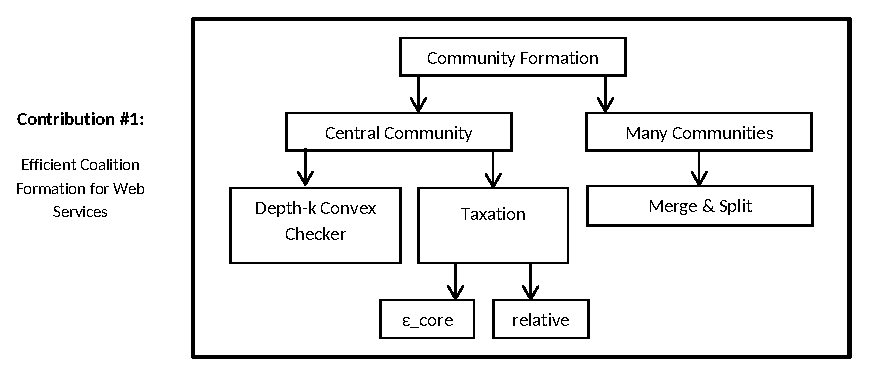
\includegraphics[width=6in]{Figures/c1.eps}`
%\caption{First contribution: Efficient Coalition Formation for Web Services}
%\label{fig_c1}
%\end{figure}
%
%\begin{figure}[!t]
%\centering
%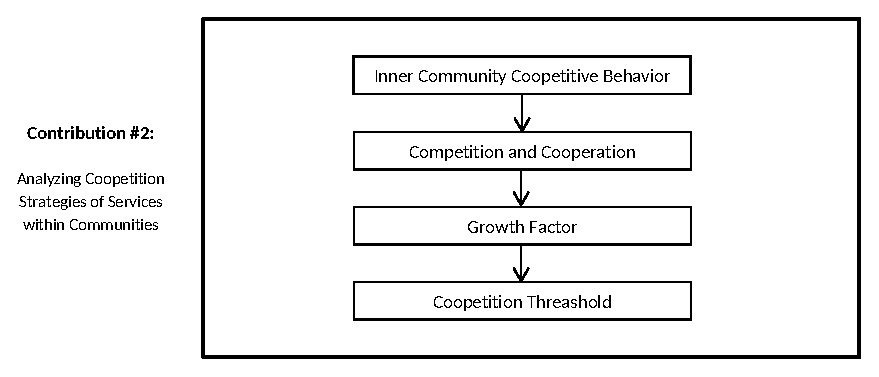
\includegraphics[width=6in]{Figures/c2.eps}`
%\caption{Second contribution: Analyzing Coopetition Strategies of Services within Communities}
%\label{fig_c2}
%\end{figure}
%
%\begin{figure}[!t]
%\centering
%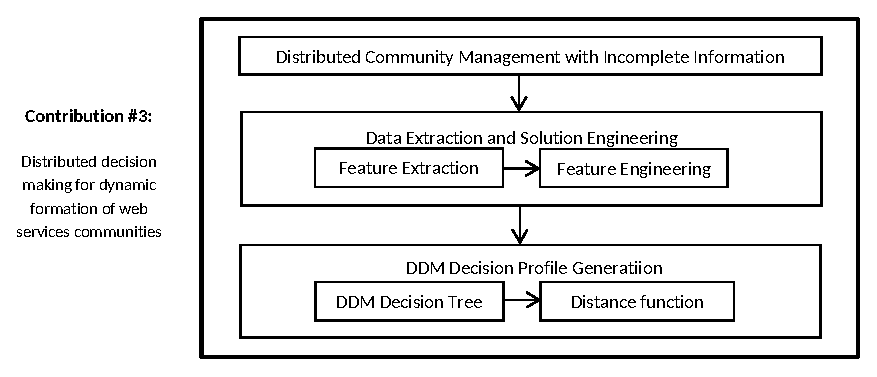
\includegraphics[width=6in]{Figures/c3.eps}`
%\caption{This contribution: Distributed decision making for dynamic formation of web services communities}
%\label{fig_c3}
%\end{figure}

Figure \ref{fig_model} highlights our contributions and proposed model for communities of web services formation and management.

\section{Thesis Organization}\label{sec:outline}
The rest of the proposal is organized as follows: We present in Chapter 2 the background needed for our research along with relevant related work. Chapter 3 provides an efficient method of coalition formation for web services. In Chapter 4 we discuss the cooperative behaviour within the communities of web services. Chapter 5 presents a distributed method of formation of web services communities. Finally in Chapter 6, we present our conclusion and future plan.


%%%%%%%%%%%%%%%%%%%%%%%%%%%%%%%%%%%%%%%%%%%%%%%%%%%%%%%%%%%%%%
%%%%%%%%%%%%%%%%%%%%%%%%%%%%%%%%%%%%%%%%%%%%%%%%%%%%%%%%%%%%%%

%
%\section{Context of Research}\label{sec:motivation_s}
%
%[seminar] Over the past years, online services have become part of many
%scalable business applications. The increasing reliance on
%web-based applications has significantly influenced the way web
%services are engineered.
%%Web services provide a set of stateless
%%software functions accessible at a network address over the web.
%%The recent developments are shifting web services from passive and
%%individual components to autonomous and group-based components
%%where interaction, composition, and cooperation are the key
%%challenges \cite{ICWS2011-1,SCC2011-1}. The main objective is to
%%achieve a seamless integration of business processes, applications
%%and web services. Delivering high quality services considering the
%%dynamic and unpredictable nature of the Internet is still a very
%%critical and challenging issue.
%%Typically, web services are business applications deployed as
%%autonomous and interoperable agents \cite{Alescio}. In fact, the
%%W3C consortium defines a web service as ``an abstract notion that
%%must be implemented by a concrete agent''. However, the web is
%%stocked with agent-based services that offer similar business
%%functionalities, which leads to service consumers having
%%difficulties in choosing the most appropriate agents to interact
%%with.
%The need for highly available and responsive services has called
%for grouping and collaborative mechanisms of loosely-coupled web
%services, particularly in business settings. The idea of grouping
%web services within communities and the way those communities are
%engineered so that web services can better collaborate have been
%proposed and investigated in
%\cite{DBLP:journals/ijebr/MaamarSTBB09,DBLP:journals/internet/BenatallahSD03,Rosario:2008:PQS:1512146.1512290}.
%Communities are virtual groups of web services having similar
%functionalities \cite{Zeng:2003:QDW:775152.775211,
%Paik:2005:TSS:2229263.2230038,Medjahed05adynamic,10.1109/ARES.2008.7},
%but probably different non-functional quality attributes, which
%form the QoS parameters.
%%When communities are used, users send
%%their requests to the masters of those communities, which are
%%responsible of managing the communities, forwarding the requests
%%to the suitable member web services and checking the credentials
%%of those members.
%Communities aim to provide higher service
%availability and performance than what individual web services can
%provide.
%%The high availability of services and the community
%%resilience to failure are guaranteed since web services can
%%cooperate and replace each other within the same community and
%%since there is no single point of failure in the communities
%%architecture.
%
%
%\section{Motivation and Research Objectives}\label{sec:motexample_s}
%
%Web service communities are dynamic by design
%\cite{DBLP:journals/ijebr/MaamarSTBB09}. In these communities, web
%services are modeled as intelligent autonomous agents, where they
%can adopt a strategy maximizing their payoff at any time. A web
%service can ask joining a community and has the right to leave it.
%Community managers can invite or ask a web service to leave in
%order to maximize the community profit. Users can simply stop
%sending requests to a web service which is not providing
%satisfactory services. Thus it is important to consider all the
%parties involved in the decision making process about the
%community management.
%
%In this research work, our first objective is to propose a
%cooperative model as game for the aggregation of web services
%within communities. The solution concepts of our cooperative game
%seeks to find efficient ways of forming coalitions (teams) of web
%services so that they can maximize their gain and payoff, and
%distribute the gain in a fair way among all the member services.
%Achieving Fairness when the gain is distributed among the
%community members is the main factor to keep the coalition stable
%as no web service will expect to gain better by deviating from the
%community. In other words, the coalition is made efficient if all
%the members are satisfied. We first propose a representation
%function for communities of web services based on their QoS
%attributes. By using this function, we can evaluate the $worth$ of
%each community of web services. When facing new membership
%requests, a typical community master checks whether the new
%coalition having the old and new set of web services will keep the
%community stable or not. The community master will reject the
%membership requests if it finds out that the new coalition would
%be unstable, preventing $any$ subset of web services from gaining
%significantly more by deviating from the community and joining
%other communities or forming new ones. The computation of
%solutions for cooperative games is combinatorial in nature and
%proven to be NP-complete \cite{Algorithmic}, making this
%computation impractical in real world applications. However, using
%the concepts of coalition stability, the second objective is to
%investigate approximation algorithms running in polynomial time
%providing web services and community masters with applicable and
%near-optimal decision making mechanisms.
%
%Within communities, services can exhibit competitive behavior as they provide the same functionalities and the number of users requests is finite.
%However, for the same reason of being functionally similar, services can cooperate with each other, for example to substitute each other in order to perform some sub-tasks.
%So as an extension of our work, we have proposed a framework in which services can opt for performing tasks if they feel they are capable enough
%or decide to cooperate by showing the availability to perform some sub-tasks.
%
%%We have implemented an online learning mechanism for services with different capabilities to learn over time which strategy to choose based on their own and other services status and capabilities. After establishing states of our model and observing convincing results from our learning method, we plan to extend the learning process using reinforcement learning (Q-learning) techniques.
%
%
%
%\indent To summarize, the main problems we aim to tackle in this
%thesis are the formation of stable and efficient coalitions
%maximizing web services and community revenue and the decision over the strategy to play about competing or cooperating.
%The main objectives are:
%\begin{itemize}
%\item To propose a cooperative model and analyze its solution
%concepts in order to address the problem of optimizing coalition
%formation for a stable community.
%
%\item To reduce the complexity of computing the solution concepts
%of the cooperative model tailored to the problem of communities of
%agent-based web services in order to make these solutions
%applicable in real world scenarios.
%
%\item To analyze the effect of different membership and taxation
%models that the master can apply to the members on the stability
%of the community.
%
%\item To investigate the impact of learning on individual and
%group decision making within the cooperative model of the
%community.
%
%\item To validate the proposed methods by extensive simulations
%and comparison with other similar proposals.
%\end{itemize}
%
%
%
%
%\section{Thesis Organization}\label{sec:outline_s}
%The rest of the thesis is organized as follows. We present in
%Chapter 111 the background needed for our research along
%with relevant related work. Chapter 222
%provides the problem statement and presents our solution model in
%two different scenarios with some preliminary results. Finally, in
%Chapter 333, we present our conclusion,
%future plan, and the timetable of our research.
%
%
%



%%%%%%%%%%%%%%%%%%%%%%%%%%%%%%%%%%%%%%%%%%%%%%%%%%%%%%%%%%%%%%%%%%%%%%%%%%%%%%%
%% Chapter 2 : Background.
%%%%%%%%%%%%%%%%%%%%%%%%%%%%%%%%%%%%%%%%%%%%%%%%%%%%%%%%%%%%%%%%%%%%%%%%%%%%%%%
\setcounter{chapter}{1}

\chapter{Background}\label{cha:background}
This chapter reviews the background needed for our thesis. We explain all concepts, techniques, and tools that are used throughout this thesis. In Section \ref{sec:social-commitment-cha2}, the concept of social commitments as a means of communication between interacting agents is discussed. Section \ref{sec:knowledge-cha2} is devoted to briefly review reasoning about knowledge in MASs. In Section \ref{sec:system-models-cha2} some modeling formalisms including Interpreted Systems, we use in this thesis, are reviewed. Temporal logics for systems specification are also presented in this section. Section \ref{sec:Model-Checking-cha2}, describes the concept of model checking. Also, a review of some prominent existing model checkers is given in this section. Finally, we conclude this chapter in Section \ref{sec:summary-chap2}.


\section{Social Commitments} \label{sec:social-commitment-cha2}
The interoperability requirement in MASs has led to the introduction of various standardized agent communication languages (ACLs). The early proposals for defining the semantics of ACLs like KQML \cite{Finin1994} and FIPA ACL\footnote{See FIPA-ACL specifications (1997,1999,2001,2002), http://www.fipa.org/repository/aclspecs.php3} are developed using agent's mental states like beliefs, desires and intentions. These are now called mentalistic approaches because their focus are on the minds of the individuals participating in the interaction. A major weakness of these approaches is that they assume that \textit{agents can read each other minds} \cite{Singh1998}. Actually, in open environments where heterogeneous agents are made by different vendors and possibility using different technologies, it seems impossible to trust other agents completely or to make strong assumptions about their internal structure. This raises a serious verification problem for such approaches \cite{Singh2008,Wooldridge2009}. To overcome this drawback, some researchers took the initiative to think about other ways for defining ACLs  \cite{Singh1998}. As a result, social commitments have come to emergence. Social commitments are basically modeled as public information conveyed by an agent to another one. More specifically, a social commitment is an agreement between an agent, namely \emph{debtor}, to another agent, \emph{creditor}, in which the debtor engages towards the creditor to bring about a certain property \cite{Castelfranchi1995,Singh2005}.
%However, despite the fact that the term of \textit{social commitments} was constructed first by Castelfranchi in \cite{Castelfranchi1995}, the notion he introduced was not purely social because it is still analyzed in terms of the mental states of the partners.
In addition to being social, commitments are also public, and objective \cite{Colombetti2000}. These properties of social commitments help heterogeneous agents attribute the same meaning to the messages being exchanged so that the meaning is expressed using concepts that do not depend on an individual agent's internal structure. Importantly, a commitment between two agents is not just a static entity, but rather a dynamic one whose state changes over time as events occurs \cite{Akin2013,Torroni2009}. This dynamicity feature supports commitments' flexibility and can be captured through the manipulation of commitments via some operations such as \emph{creation}, \emph{fulfillment},
\emph{cancellation}, \emph{release}, \emph{assignment}, and
\emph{delegation} \cite{Singh1999}. In particular, a debtor may \emph{create} a commitment, thus activating it, or \emph{fulfill} a commitment, thus discharging it. However, for different reasons, a debtor might fail to fulfill its commitment; thus, it becomes violated. Given a commitment, its creditor can freely \emph{assign} it to another creditor, and its debtor may \emph{delegate} it to a another debtor. Furthermore, a debtor may \emph{cancel} a commitment; whereas, a creditor can \emph{release} the debtor from the commitment at any time.

%

%The notion of commitments as a foundation for understanding interactions among agents has been under development for about twenty years

Commitment-based approaches to ACLs have been around for about twenty years. Defining semantics of ACLs using the notion of social commitments has its roots back to the work of Singh \cite{Singh2000} in which he was the first to formalize a commitment-based ACL in temporal logic. Since then, social commitments have gained more and more popularity as a communication approach that makes no assumptions on the agents' internal states. To develop such approaches, various commitment logics that extend CTL (Computation Tree Logic), LTL (Lineal Temporal Logic), and CTL$^{*}$ (superset of CTL and LTL) have been introduced. Examples of efforts on this line can be found in
\cite{Bentahar2004,Giordano2007,Pham2007,Singh2000,Verdicchio2003}.
These logics have been successful in specification
and verification of systems from different areas such as
commitment-based protocols
\cite{Baldoni2010,El-Menshawy2010,Fornara2004b,Yolum2004},
modeling business processes \cite{Desai2009,Telang2009} and
agent-based web services \cite{Bentahar2008}.
However, the common limitation of theses proposals is that they neglect the uncertainty aspects of MASs and tend to assume typical behavior instead. In broad terms, uncertainty is a crucial aspect in MASs and has an impact not only on the behavior of the participating agents but also on the communication process that occur among these agents. %In Chapter \ref{cha:PCTLC}, we propose a new probabilistic logic whose primary purpose is to represent and reason about commitment-based agent communication in the presence of uncertainty.

In this thesis, we consider the notion of ``social commitments'' that is meant for communication. That is, the notion of commitments as a foundation for understanding interactions among agents. Therefore, we use communicative social commitments, also called illocutionary social commitments, as defined in \cite{Bentahar2012,El-Menshawy2013a}. Those commitments are formally denoted by $C_{i \to j} \varphi$, meaning that agent $i$, the debtor, commits to agent $j$, the creditor, to bring about $\varphi$, where $\varphi$ is the content of the commitment. Different notations with the same meaning can be found in \cite{Desai2009,Fornara2004a,Singh2000}.
This notion of ``social commitments'' should not be confused with some related notions such as ``Internal Commitments'', ``Norms'', and ``Obligations''. In traditional Artificial Intelligence (AI), a commitment was understood as the commitment of a single agent to some belief or to some course of action \cite{Levesque1990}. In this direction, ``internal commitment'' \cite{Castelfranchi1995,Singh2008} which refers to a commitment of an agent to itself has been widely used in the domain of AI. Norms, which are formal specifications of deontic statements that aim at regulating the interactions among agents, have also received a considerable attention in AI and MASs domains \cite{Balke2013,Singh2013,Testerink2013}. Obligations, on the other hand, have long been used as explicit mechanisms for influencing the behavior of interacting parties and providing some stability and reliability in their interactions \cite{Dignum2002}. Some researchers consider that commitments are somewhat like direct obligations \cite{Dignum1996,Singh2008}.

In contrast, the interesting feature that differentiates social commitments from the aforementioned notions is that a social commitment is directed from one party (the debtor) to another one (the creditor) which reflects the intuition that the debtor is committed to doing something for the creditor. These commitments are illocutionary in the sense that they are used as means of conveying information among interacting agents. Moreover, communicative commitments are equipped with a grounded semantics because the social accessibility relation has an intuitive and computational interpretation that makes its model checking possible.
%However, though Castelfranchi  tried to construct the notion of ``social commitment'', but it not purely social as it is yet analyzed in terms of the mental states of the partners \cite{Castelfranchi1995}. Another type of commitments introduced in AI before







\section{Reasoning about Knowledge} \label{sec:knowledge-cha2}

knowledge logics (also known as epistemic logics) are focused on reasoning about the knowledge that agents may have about themselves, the world, or other agents \cite{Fagin1995}. These logics have been shown to be a useful framework for the analysis of distributed algorithms and security protocols. Generally, an epistemic logic captures the essence of knowledge through modal operators. In this line, the contribution of Jaakko Hintikka in \cite{Hintikka1962} is recognized as the first attempt to investigate the logic of knowledge as a modal logic. Since then, researchers in AI and MASs have carried out numerous proposals to represent the evolution of knowledge \cite{Delgado2009,Fagin1995,Halpern2003,Huang2011,Lomuscio2007,Lomuscio2012,Meyer1995,Wan2013}. Formally, agent $i$ knows something is denoted by $K_i~\varphi$. From a verification perspective, model checking the logic of knowledge was first mooted by Halpern and Vardi \cite{Halpern1991}. Since that time theoretical aspects of model checking the logic of knowledge and its combinations with temporal logic have been studied. %Most existing solutions combine the logic of knowledge with LTL and/or CTL temporal logics.

In addition to reasoning about what one agent knows, it is often useful to be able to reason about the \textit{common knowledge}: the things that everyone knows, and that everyone knows that everyone knows, etc. Everyone knows can be defined as an abbreviation:

\noindent $E_G \varphi \equiv K_1 \varphi \wedge \dots K_n \varphi$, where $G$ is a group of agents, and $n$ is the number of agents in $G$.

\noindent The common knowledge operator $C_G$ is defined in terms of $E_G$ as follows:

\noindent $C_G \equiv E_G \varphi \wedge E_G^2 \varphi \wedge \dots \wedge E_G^k \wedge \dots $, where $E_G^k$ is read: ``everyone in $G$ knows $\varphi$ to degree k''.




\section{Modeling Techniques} \label{sec:system-models-cha2}
Transition Systems (TSs) are typically used as models to describe the behavior of systems \cite{Clarke1999}. They are the underlying models for all various non-real time models. TSs are modeled as directed graphs where nodes reflect the states, and edges represent the transitions. A state describes some information about the systems at a given moment of its behavior. Whereas, a transition describes how the systems can evolve from one state to another. A TS is a tuple $\mathbb{T} =(S, Act, \rightarrow, I, AP, \mathrm{L})$, where $S$ is a set of states, $Act$ is a set of actions, $\rightarrow\subseteq S\times Act \times S$ is the transition relation, $I\subseteq S$ is a set of initial states, $AP$ is a set of atomic propositions, and $\mathrm{L}: S \to 2^{AP}$ is a labeling function \cite{Baier2008}. %In Kripke structure \cite{Clarke1999}, $\mathrm{L}$ is introduced into TS to label states. However, in this section, we review some computational models that are used for modeling probabilistic systems.
In order to model random phenomena, transition systems are enriched with probabilities. This can be done in different ways. In the rest of this section, we review some probabilistic models that are used throughout our thesis.

\subsection{Interpreted Systems} \label{interpreted-systems-cha2}

The formalism of interpreted systems introduced by Fagin el al. \cite{Fagin1995} provides a useful framework to locally
model autonomous and heterogeneous agents who interoperate within
a global system via sending and receiving messages. This thesis builds on this formalism for various reasons:

\begin{itemize}
\item It is a suitable formalism for modelling agent-based systems as it provides a good level of abstraction that allows focusing more on modeling the key characteristics of the interacting agents along the evolution of their social commitments \cite{El-Menshawy2012}.
\item It has been successfully used to reason about various aspects of MASs such as time, knowledge, commitments, and correct behavior.
\item Interpreted systems are computationally grounded \cite{Wooldridge2000b}, meaning that the semantics of interpreted systems maps directly to the paths of the system, and vice-versa.
\item Interpreted systems can be easily extended. The original version introduced by Fagin et al. \cite{Fagin1995} has been extended in various ways as we will see below. This property of being readily extensible is important for us as we always need to extend it as required.
\end{itemize}

Suppose a set $\texttt{Agt}=\{1,\ldots,n\}$ of $n$
agents. At all times, each agent in the system is assumed to be in
some \textit{local} state, which intuitively records the complete
information that the agent can access at that time. Specifically,
each agent $i\in \texttt{Agt}$ is characterized by countable sets
$L_i$ and $Act_i$ of local states and actions respectively in
which the set $Act_i$ is mainly used to account for the temporal
evolution of the system. Also, local actions for each $i\in
\texttt{Agt}$ are performed in compliance with a local protocol
$\mathcal{P}_i: L_i\rightarrow 2^{Act_i}$, which assign a set
of enabled local actions to a local state. Intuitively, this set corresponds to the actions that are enabled in a given local state. Furthermore, the environment in which agents live may be modeled by means of a special agent $e$. Associated with $e$ are a set of local states
$L_e$, a set of actions $Act_e$, and a protocol $\mathcal{P}_e$. A
tuple $g = (l_1,\ldots, l_n,l_e) \in (L_1\times \ldots \times
L_n\times L_e)$ where $l_i\in L_i$ for each $i\in \texttt{Agt}$
and $l_e\in L_e$, is called a ``global state'' and represents the
instantaneous configuration of all agents in the system at a given
time (i.e., a snapshot of the global system at a specific time).

The local evolution function $\tau_i$ that determines the
transitions for an individual agent $i$ between its local states
is defined as follows:
%
\begin{equation}
\tau_i : L_i\times L_e\times Act_i \rightarrow L_i
\end{equation}
%
Similarly, the global evolution function of the system is defined as follows:
%
\begin{equation}
\tau : G\times ACT\rightarrow G
\end{equation}
%
where $ACT=Act_1 \times \ldots \times Act_n$ and each component
$a\in ACT$ is called a ``joint action'', which is a tuple of
actions (one for each agent), and $G = L_1\times \ldots\times
L_n\times L_e$ denotes a set of global states. The notation
$l_i(g)$ is used to represent the local state of agent $i$ in the
global state $g$. In addition, $I\in G$ is an initial global state
for the system. %For simplification, we remove the environment agent from the interpreted system formalism as done in \cite{Lomuscio2007}.

Bentahar et al. \cite{Bentahar2012} and El-Menshawy et al. \cite{El-Menshawy2013a} extended Fagin et al.'s formalism of interpreted systems with shared and unshared variables in order to account for communication that occurs during the execution of MASs and to provide an intuitive semantics for social commitments that are established through communication between interacting agents. They specifically associated with each agent $i\in \texttt{Agt}$ a countable set $Var_i$ of local
variables. Then, they used those variables to represent
communication channels through which messages are sent and
received. Technically, they denoted the value of a variable $x$ in
the set $Var_i$ at local state $l_i(g)$ by $l^{x}_i(g)$. Thus,
%
\begin{equation}
\textrm{if}~ l_i(g)=l_i(g'),~\textrm{then}~ l^{x}_i(g)
=l^{x}_i(g')~ \textrm{for~all}~ x \in Var_i
\end{equation}
%
The idea is that, for two agents $i$ and $j$ to communicate, they
should share a communication channel, which is represented by
shared variables between $i$ and $j$. In this perspective, a
communication channel between $i$ and $j$ does exist iff $Var_i
\cap Var_j \neq\emptyset$. For a variable $x \in Var_i \cap
Var_j$, $l^{x}_i(g)=l^{x}_j(g')$ means the values of $x$ in
$l_i(g)$ for agent $i$ and in $l_j(g')$ for agent $j$ are the same. This
intuitively represents the existence of a communication channel
between $i$ (in $g$) and $j$ (in $g'$) through which the variable
$x$ has been sent by one of the two agents to the other, and as a
consequence of this communication, $i$ and $j$ will have the same
value for this variable. The key point is that shared variables
are only used to motivate the existence of communication channels,
not the establishment of communication. Figure \ref{fig:social accessibility-cha2} depicts the idea of using shared and unshared variables for establishing communication channels between interacting agents.
The three conditions upon which a communication channel between $i$ and $j$ exists are listed below:

For each pair $(i,j) \in \texttt{Agt}^2$, $\sim_{i\rightarrow j} \subseteq S \times S$ is a social accessibility relation. $s \sim_{i\rightarrow j} s'$ is defined by the following conditions:
      %
  \begin{enumerate}
       \item $l_i(s)=l_i(s')$.
       \item $Var_i \cap Var_j \neq \emptyset$ such that $\forall x \in Var_i \cap Var_j$ we have $l^{x}_i(s)\!=\!l^{x}_j(s')$.
       \item $\forall y \in Var_j\!-\! Var_i$ we have $l^{y}_j(s)\!=\!l^{y}_j(s')$.
  \end{enumerate}

    %\begin{figure}[t]
    \begin{figure}[!ht]
                \begin{center}
                \includegraphics[width=12cm, %height=7cm]{chap2/img/social-accessibility-cha2.eps}
                height=7cm]{chap2/img/social-accessibility1.eps}
                \end{center}
                \caption{Social accessibility relations as defined in \cite{Bentahar2012,El-Menshawy2013a}}
                \label{fig:social accessibility-cha2}
    \end{figure}

Recently, Al-Saqqar et al. \cite{Al-Saqqar2014a} have modified the definition of social accessibility relations given in \cite{Bentahar2012,El-Menshawy2013a} in such a way that the new definition does no longer depend on the unshared variables but rather depends merely on the shared variables between the interacting agents as shown in Figure \ref{fig:modified social accessibility-cha2}. The new condition upon which a communication channel is established is stated below:

 $ s \approx_{i \rightarrow j} s' $ iff $ Var_i \cap Var_j \neq \emptyset $ such that $ \forall x \in Var_i \cap Var_j $ we have $ l_i^x(s) =
l_i^x(s') = l_j^x(s')$, where $\approx_{i\rightarrow j} \subseteq S \times S$ is the new social accessibility relation \cite{Al-Saqqar2014a}.

%\begin{figure}[t]
    \begin{figure}[!ht]
                \begin{center}
                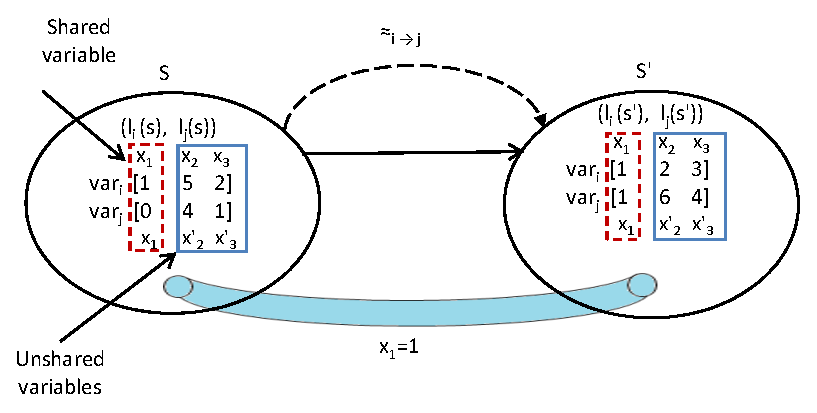
\includegraphics[width=12cm, height=7cm]{chap2/img/social-accessibility2.eps}
                \end{center}
                \caption{The modified version of social accessibility relations as in \cite{Al-Saqqar2014a}}
                \label{fig:modified social accessibility-cha2}
    \end{figure}


The original version of interpreted systems formalism was also extended by Halpern et al. \cite{Halpern2003} and further by Wan et al. \cite{Wan2013} to model the stochastic behavior of MASs. Accordingly, the local evolution function is defined as follows:
%
\begin{equation}
\tau_i: L_i \times Act_i \times L_i \rightarrow[0,1]
\end{equation}
%
such that for all $l_i \in L_i$, we have $\sum_{l'_i\in L_i}
\tau_i(l_i,a^{l_i\rightarrow l'_i},l_i')=1$ wherein
$a^{l_i\rightarrow l'_i}$ is the local action labeling a
transition between local states $l_i$ and $l'_i$ of agent $i$.


Moreover, the global evolution function is defined as follows:
%
\begin{equation}
\tau: G \times ACT \times G \rightarrow[0,1]
\end{equation}
%
%This function satisfies Markovian properties in the sense that
The sum of the probabilities over all possible transitions from a given state $g$ must be $1$: for all $g \in G$, $\sum_{\substack{g'\in G}}
\tau(g,a^{g\rightarrow g'},g')=1$ where $a^{g\rightarrow g'}$ is
the action labeling the transition between the two global states
$g$ and $g'$ of the system.

Such a modified version of the interpreted systems formalism is
called \textit{probabilistic interpreted systems}
\cite{Halpern2003}. In the formalism of probabilistic interpreted
systems, the transition probability matrix can be computed by
\cite{Wan2013}:

\begin{equation}\label{global-evo-fun}
\tau(g,a^{g\rightarrow g'},g')= {\prod_{\substack{i \in
\texttt{Agt}}} \tau_i(l_i(g), a^{l_i(g) \rightarrow
l_i(g')},l_i(g'))}
\end{equation}




\subsection{Discrete Time Markov Chains (DTMCs)} \label{sec:DTMC-cha2}

DTMCs are commonly used as models for probabilistic systems. A DTMC is a transition system that defines the probability of moving from one state to another.
\begin{definition}[DTMC]\label{def:DTMC}
Given a set of atomic propositions $AP$, a DTMC can be defined as a 4-tuple
$\mathbf{D}$ = $(S,\overline{s},\mathbf{P},L)$ where:

\begin{itemize}
  \item  $S$ is a nonempty and finite set of states;
  \item  $\overline{s}$ is the initial state;
  \item  $\mathbf{P} :  S\times S\rightarrow[0,1]$ is the transition
  probability matrix, such that for every state $s\in{S}$, we have
  $ \sum_{s' \in{S}} \mathbf{P}(s,s' )=1$;
  \item  $L : S\rightarrow 2^{AP}$  is a labelling function which assigns to each state $s \in S$ the set $L(s)$ of atomic propositions that are valid in the state.
\end{itemize}
\end{definition}


DTMCs are stochastic models of systems that change their states at discrete-times $(n=0,1,2,\dots)$ and have the following property: if the system enters state $s$ at time $n$, it stays there for exactly one unit of time and then jumps to state $s'$ at time $n+1$ with probability $\mathbf{P}(s, s')$, regardless of its history up to and including time $n-1$ \cite{Kulkarni1995}. The definition shows that states are labelled with atomic propositions which indicate the status of the system (e. g., waiting, sending). The system can change its states according to a probability distribution given by the transition probability matrix $\mathbf{P}$. Each element $\mathbf{P} (s,s')$ of the transition probability matrix gives the probability of making a transition from state $s$ to state $s'$. A transition from state $s$ to $s'$ can only take place if $\mathbf{P}(s, s') > 0$. However, if $\mathbf{P}(s, s') = 0$, no such transition is possible. Again, the probabilities from a given state must sum up to 1, i.e. $\sum_{s' \in{S}} \mathbf{P}(s,s' )=1$.


\subsection{Markov Decision Processes (MDPs)} \label{sec:MDP-cha2}
MDPs can be seen as transition systems in which in any state a nondeterministic choice between probability distributions exists.

\begin{definition}[MDP]\label{def:MDP}

Given a set of atomic propositions $AP$, an MDP model $\mathbf{M}$ can be defined as a 5-tuple, $\mathbf{M}$ = $(\mathbb{S}, AC, \textsf{P}_t ,I_i, L)$, where:

\begin{itemize}

  \item  $\mathbb{S}$ is a nonempty and finite set of states.

  \item  $\textsf{P}_t:  \mathbb{S}\times AC\times \mathbb{S}\rightarrow[0,1]$ is the transition probability function, such that for every state $s\in{\mathbb{S}}$ and action $\theta \in AC$, we have $\sum_{s' \in{\mathbb{S}}} \textsf{P}_t(s,\theta ,s') \in \{0,1\}$.

  \item  $AC $ is a set of actions. At state $s \in \mathbb{S}$, the action $\theta$ is enabled iff $\sum_{s' \in{\mathbb{S}}} \textsf{P}_t(s,\theta ,s')=1$.

  \item  $I_i$ is an initial state.

  \item  $L : \mathbb{S}\rightarrow 2^{AP}$  is a state labeling function.
\end{itemize}
\end{definition}

MDPs possess the Markov property, which requires that any information necessary to predict the effects of all events is captured in the state. In other words, the effects of an event in a state depend only on that state and not on the prior history. However, the major difference between MDPs and DTMCs is the choice of actions. While a DTMC describes the state transitions of a stochastic system, it does not capture the fact that the agent can choose an appropriate course of action in order to change the system's state. However, for an MDP, at every state one or more actions are available, and each action is associated with a probability distribution over the successor states. That is, MDPs are not augmented with a unique
probability measure. Reasoning about probabilities of sets of
paths of an MDP relies on the resolution of the nondeterminism. In
order to define the semantics of such an MDP, the notion of \textit{adversary} is used. An adversary (also referred to as scheduler, policy, or strategy \cite{Baier2008,Vardi1985}) is an entity that resolves the nondeterministic choices in MDPs. Being in a state of the system, an adversary determines the next step to be taken. %Hence, the adversary is used the notion of adversary to factor out the nondeterminism and consider the probability of some behavior of the MDP \cite{Forejt2011}.
Informally, at each step, the adversary picks an action, and then the next
state is picked according to the probability distribution
associated with the action. In our work, we focus on a special
class of adversaries called \emph{Memoryless Adversary} \cite{Forejt2011} where the choice of action depends only on the state and independent of what has happened in the history. An adversary is said to be memoryless if it always selects the same action in a given state. The induced adversaries are basically DTMC models.

A partially observable Markov decision process (POMDP) is a variant of MDPs. Actually, a POMDP is an MDP in which the agent is unable to observe the current state. Instead, the agent must maintain a probability distribution over the set of possible states, based on a set of observations and observation probabilities, and the underlying MDP. A POMDP model \cite{Kaelbling98} can be described as a tuple $(\mathrm{S},\mathbb{A},\mathrm{T},\mathbf{R},\Omega,\mathrm{O})$, where:

\begin{itemize}

  \item $\mathrm{S}$, $\mathbb{A}$, $\mathrm{T}$, and $\mathbf{R}$ describe an MDP;
  \item $\Omega$ is a finite set of observations that the agent can experience of its world; and
  \item $\mathrm{O}: \mathrm{S} \times \mathbb{A}\to \prod(\Omega)$ is the observation function, which gives, for each action and resulting state, a probability distribution over possible observations.

\end{itemize}



\section{System Specification} \label{sec:sys-spec-cha2}
In this section, we describe some logics for specifying requirements of transition-based systems. The discussed logics use atomic propositions and connective operators to describe systems properties in states.

\subsection{Temporal Logics}
Temporal logic is a modal logic with modal operators to describe the temporal order of occurrence of events. The two commonly used temporal logics are Linear Temporal Logic (LTL) \cite{Pnueli1977} and Computation Tree Logic (CTL) \cite{Emerson1990}. They differ from each other based on the way the notion of time is handled. LTL describes temporal relations on one execution path; whereas, in CTL it is possible to quantify over the paths with respect to a given state. Below, we review the two logics and then review a probabilistic extension of CTL called PCTL \cite{Hansson1994}.



\noindent \textbf{a. LTL (Linear Temporal Logic)}

In LTL, time is considered to be a linear sequence. Each moment in time has a unique possible future. Thus, temporal operators are provided for describing events along a single time line. The syntax of LTL is defined by the following BNF grammar \cite{Baier2008}:
%
\begin{align*}
    \varphi & ::= true ~|~p~|~\neg \varphi~|~\varphi \wedge \varphi~|~ \bigcirc \varphi ~ | ~ \varphi ~U~ \varphi~|
\end{align*}

\noindent where: $p\in AP$ is an atomic proposition. $\bigcirc$ and $\mathrm{U}$ stand for ``next time'' and ``until'' respectively. The formula $\bigcirc \varphi$  holds at the current state if $\varphi$ holds in the next state. The formula $\varphi U \psi$ holds at the current state, if there is some future moment for which $\psi$ holds and $\varphi$ holds at all moments until that future moment. $\lozenge \varphi$, which stands for eventually $\varphi$ holds, can be derived using the $\mathrm{U}$ operator as follows: $\lozenge \varphi \equiv \mathrm{true}~ \mathrm{U}~ \varphi$. Also, the $\square \varphi$, which stands for ``always $\varphi$, or  globally $\varphi$'', can be derived as follows: $\square \varphi \equiv \neg\lozenge~ \neg\varphi$. The Boolean connectives $\neg$ and $\vee$ are defined in the usual way.

\noindent \textbf{Semantics of LTL.} Formulae of LTL stand for properties of paths. Therefore, a path can either satisfy an LTL-formula or not. Let $\mathbb{T} =(S, Act, \rightarrow, I, AP, \mathrm{L})$ be a transition system where $S$ is a nonempty set of states, $Act$ is a set of actions, $\rightarrow\subseteq S\times Act \times S$ is the transition relation, $I\subseteq S$ is a set of initial states, $AP$ is a set of atomic propositions, and $\mathrm{L}: S \to 2^{AP}$ is a labeling function. Given $s,s' \in S$, $(s,s') \in \rightarrow$ means that $s'$ is an immediate successor of $s$. A path $\pi$ in $\mathbb{T}$ is an infinite sequence of states $\pi=(s_0,s_1,\dots)$ such that $(s_i,s_{i+1})\in \rightarrow$ for all $i\geq 0$. $\pi(i)$ is the $(i+1)$-th state in $\pi$, and $\pi_i = \pi(i), \pi(i+1), \dots$ is the suffix of $\pi$ starting at $\pi(i)$. The satisfaction of an LTL-formula $\varphi$ with respect to the path $\pi$ in the transition system $\mathbb{T}$ is denoted by $(\mathbb{T},\pi) \models \varphi$, which is inductively defined as follows:

\noindent $-~(\mathbb{T},\pi) \models p ~~~~~~~~~~~~~\emph{iff}~~~ p\in \mathrm{L}(\pi(0)),$\\
$-~(\mathbb{T},\pi) \models \neg \varphi ~~~~~~~~~~\emph{iff}~~~ (\mathbb{T},\pi)\nvDash \varphi,$\\
$-~(\mathbb{T},\pi) \models \varphi_1 \wedge \varphi_2 ~~~~\emph{iff}~~~(\mathbb{T},\pi)\models \varphi_1~\textrm{and}~(\mathbb{T},\pi) \models \varphi_2,$ \\
$-~(\mathbb{T},\pi) \models \bigcirc\varphi ~~~~~~~~~\emph{iff}~~~ (\mathbb{T},\pi(1)) \models \varphi,$\\
$-~(\mathbb{T},\pi) \models (\varphi_1~U~\varphi_2)~~\emph{iff}~~\exists~ k \geq 0~~\textrm{such that}~~ (\mathbb{T},\pi(k)) \models \varphi_2 ~\textrm{and}~\forall~ 0\leq i < k, (\mathbb{T},\pi(i)) \models \varphi_1$.

\noindent An LTL-formula $\varphi$ holds at state $s$ in the model $\mathbb{T}$, written $(\mathbb{T},s) \models \varphi$, iff all paths starting from $s$ satisfy $\varphi$. Moreover, the model $\mathbb{T}$ satisfies $\varphi$ iff $\varphi$ holds in all paths emanating from an initial state. We say that $\varphi$ is valid in $\mathbb{T}$, written $\models \varphi$ when for all $s\in S$, we have $(\mathbb{T},s)\models \varphi$.

\noindent \textbf{b. CTL (Computation Tree Logic)}

In contrast to LTL, CTL advocates a tree-like structure time, allowing some instants to have more than a single successor. Thus, it distinguishes between state formulae and path formulae. The syntax of CTL is given by the following BNF grammar \cite{Baier2008}:
%
\begin{align*}
    \varphi & ::= true ~|~p~|~\neg \varphi~|~\varphi \wedge \varphi~|~\mathrm{E}\psi~|~\mathrm{A} \psi\\
    \psi & ::=\bigcirc \varphi ~ | ~ \varphi ~U~ \varphi~|
\end{align*}

\noindent Intuitively, state formulae express a property of a state, while a path formulae express a property of a computation path where a computation path is an infinite sequence of states. $\bigcirc$ and $\mathrm{U}$ are defined as in LTL. Notice that, in CTL, a path quantifier (either $\mathrm{A}$ which stands for \textit{all paths}, or $\mathrm{E}$ which stands for \textit{some path}) is immediately followed by a single one of the usual linear
temporal operators $\Box$, $\lozenge$, $\bigcirc$, or $\mathrm{U}$ in order to construct a well formed state formula.

\noindent \textbf{Semantics of CTL.} The semantics of CTL is given via the satisfaction relation ``$\models$''. Given a transition system $\mathbb{T} =(S, Act, \rightarrow, I, AP, \mathrm{L})$, where $S$ is a nonempty set of states, $Act$ is a set of actions, $\rightarrow\subseteq S\times Act \times S$ is the transition relation, $I\subseteq S$ is a set of initial states, $AP$ is a set of atomic propositions, and $\mathrm{L}: S \to 2^{AP}$ is a labeling function. A path $\pi$ in $\mathbb{T}$ is also an infinite sequence of states $\pi=(s_0,s_1,\dots)$ such that $(s_i,s_{i+1})\in \rightarrow$ for all $i\geq 0$. $\pi(i)$ is the $(i+1)$-th state in $\pi$, and $\pi_i = \pi(i), \pi(i+1), \dots$ is the suffix of $\pi$ starting at $\pi(i)$. The set of paths starting at state $s$ is denoted by $\Pi(s)$. The satisfaction relation $(\mathbb{T},s)\models \varphi$, which means that the formula $\varphi$ holds at the state $s$ in the model $\mathbb{T}$, is defined inductively as follows:


\noindent $-~(\mathbb{T},s) \models p ~~~~~~~~~~~~~~\emph{iff}~~~ p\in \mathrm{L}(s),$\\
$-~(\mathbb{T},s) \models \neg \varphi ~~~~~~~~~~~\emph{iff}~~~ (\mathbb{T},s)\nvDash \varphi,$\\
$-~(\mathbb{T},s) \models \varphi_1 \wedge \varphi_2 ~~~~~\emph{iff}~~~(\mathbb{T},s)\models \varphi_1~\textrm{and}~(\mathbb{T},s) \models \varphi_2,$ \\
$-~(\mathbb{T},s) \models \exists \psi ~~~~~~~~~~~\emph{iff}~~~ (\mathbb{T},\pi) \models \psi ~\textrm{for~some}~ \pi \in \Pi(s),$\\
$-~(\mathbb{T},s) \models \forall \psi ~~~~~~~~~~~\emph{iff}~~~ (\mathbb{T},\pi) \models \psi ~\textrm{for~all}~ \pi \in \Pi(s).$

\noindent Like LTL, the satisfaction relation $\models$ for path formulae is defined by:

\noindent $-~(\mathbb{T},\pi) \models \bigcirc\varphi ~~~~~~~~~~\emph{iff}~~~ (\mathbb{T},\pi(1)) \models \varphi,$\\
$-~(\mathbb{T},\pi) \models (\varphi_1~U~\varphi_2)~~\emph{iff}~~\exists~ k \geq 0~~\textrm{such that}~~ (\mathbb{T},\pi(k)) \models \varphi_2 ~\textrm{and}~\forall~ 0\leq i < k, (\mathbb{T},\pi(i)) \models \varphi_1$.


\noindent State formula $\exists \psi$ is valid in state $s$ if and only if there exists some path starting in $s$ that satisfies $\psi$. In contrast, state formula $\forall \psi$ is valid in state $s$ if and only if all paths starting in $s$ satisfy $\psi$.

\noindent \textbf{c. PCTL (Probabilistic Computation Tree Logic)}

PCTL \cite{Hansson1994} is an extension of CTL with a probability operator. It is used to express properties of probabilistic systems. The syntax of PCTL is defined by the following BNF grammar \cite{Baier2008}:
%
\begin{align*}
    \varphi & ::= true ~|~p~|~\neg \varphi~|~\varphi \wedge \varphi~|~ \mathbb{P}_{\bowtie k} (\psi)~\\
    \psi & ::=\bigcirc \varphi ~ | ~ \varphi ~U~ \varphi~|~ \varphi~ U^{\leq m} ~ \varphi
\end{align*}

\noindent where: $p\in AP$ is an atomic proposition and $\mathbb{P}_{\bowtie k}$ is a probabilistic operator. $\bowtie \in\{<,\leq,>,\ge\}$. $k\in [0,1]$ is a probability bound or threshold. $m \in\mathbb{N}^+ $ is a positive integer number reflecting the maximum number of transitions needed to reach a certain state. $\varphi$ and $\psi$ are state and path formulae respectively. $\bigcirc, U$ and $U^{\leq m}$ stand for ``next time'',
``until'' and ``bounded until'' path modal connectives respectively.

\noindent \textbf{Semantics of PCTL.} Given a probabilistic model such as a Markov chain $\textbf{M} =(S,\verb"P",I,AP,L)$ where $S$ is a finite set of states, \verb"P" is the transition probability matrix, $I\subseteq S$ is a set of initial states, $AP$ is a set of atomic propositions, and $\mathrm{L}: S \to 2^{AP}$ is a labeling function. Let $\varphi$ and $\psi$ be PCTL state and path formulae respectively. The satisfaction relation $\models$ is defined for a PCTL state formula $\varphi$ inductively as follows:

\noindent $-~(\textbf{M},s) \models p ~~~~~~~~~~~~~~\emph{iff}~~~ p\in \mathrm{L}(s),$\\
$-~(\textbf{M},s) \models \neg \varphi ~~~~~~~~~~~\emph{iff}~~~ (\textbf{M},s)\nvDash \varphi,$\\
$-~(\textbf{M},s) \models \varphi_1 \wedge \varphi_2 ~~~~~\emph{iff}~~~(\textbf{M},s)\models \varphi_1~\textrm{and}~(\textbf{M},s) \models \varphi_2,$ \\
$-~(\textbf{M},s \models \mathbb{P}_{\bowtie k} (\psi)~~~~~~\emph{iff}~~Prob_s(\psi)\bowtie k, \textrm{where:}~Prob_s(\psi)=Prob_s\{\pi \in \Pi(s)~|~\pi\models
\psi\}.$

\noindent For a path $\pi \in \textbf{M}$, the satisfaction relation is defined as follows:

\noindent $-~(\textbf{M},\pi) \models \bigcirc \varphi~~~~~~~~~~~~~\emph{iff}~~(\textbf{M},\pi(1)) \models \varphi,$ \\
$-~(\textbf{M},\pi) \models \varphi_1~U^{\leq  m}~\varphi_2~~~\emph{iff}~~\exists~ k \leq m~~\textrm{s.t.}~~ \pi(k) \models \varphi_2 ~\textrm{and}~\forall i < k, (\textbf{M},\pi(i)) \models \varphi_1,$\\
$-~(\textbf{M},\pi) \models \varphi_1 ~U~\varphi_2~~~~~~~~\emph{iff}~~\exists~ m \geq 0~~\textrm{s.t.}~~(\textbf{M},\pi) \models \varphi_1~U^{\leq m}~\varphi_2.$\\


\noindent \textbf{Combining Logics}

Logic combination is emerging as a relevant research topic in many disciplines. Multi-modal logics can be constructed by combining existing logics in several ways \cite{Gabbay2003}. In this thesis, we advocate the independent join (or fusion) technique \cite{Franceschet2004}. The problem of combining logics based on the independent join technique is as follows. Given two logics $\mathbf{A}$ and $\mathbf{B}$, how do we
combine them into one logic which extends the expressive power of each one?

The combination of two logics using this technique is denoted by $\mathbf{A} \oplus \mathbf{B}$.
Given two logics $\mathbf{A}$ and $\mathbf{B}$, their languages
$\mathcal{L}_\mathbf{A}$ and $\mathcal{L}_\mathbf{B}$, and their corresponding axiomatic systems $\mathcal{H}_\mathbf{A}$ and $\mathcal{H}_\mathbf{B}$, the logic $\mathbf{A} \oplus \mathbf{B}$ is the smallest logic with the following properties:

\begin{itemize}
\item The language of the combined logic is the union of $\mathcal{L}_\mathbf{A}$ and $\mathcal{L}_\mathbf{B}$.
\item The resultant logic from the combination is axiomatised by the set of axioms $\mathcal{H}_\mathbf{A} \cup \mathcal{H}_\mathbf{B}$ which means that no ``interaction'' axiom is needed, i.e., axioms involving mixed operators are not necessarily required.

\end{itemize}


If $\mathcal{L}_\mathbf{A}$ and $\mathcal{L}_\mathbf{B}$ are interpreted in Kripke frames $\mathrm{F}_1 = (W,R_{11}, \dots ,R_{1n})$ and $\mathrm{F}_2 = (W,R_{21}, \dots ,R_{2m})$ , the semantics of the combined logic $\mathbf{A} \oplus \mathbf{B}$  can be interpreted over the Kripke frame $\mathrm{F} = (W,R_{11}, \dots ,R_{1n},R_{21}, \dots, R_{2m})$ obtained by the ``fusion'' of the two frames $\mathrm{F}_1$ and $\mathrm{F}_2$.
Using this technique ensures the preservation of important properties (such as soundness, completeness, and decidability, etc.) of the logics being combined as they are defined in the literature \cite{Konur2013}.




\section{Model Checking} \label{sec:Model-Checking-cha2}

Verification is one of the important aspects of ACLs. Generally, for ACL standards to gain acceptance, it must be possible to determine whether or not any agent-based system that claims to conform to an ACL standard actually does so. An ACL is said to be verifiable if it enjoys this property \cite{Wooldridge1998,Wooldridge2000}. In this section, we review a verification technique, namely model checking, that is utilized in this research to verify our proposed logics.

%Model checking is most widely understood as a technique for automatically verifying that finite state systems satisfy formal specifications.

Model checking is a formal, automatic technique to verify whether
or not system design models satisfy given requirements \cite{Bordini2006,Clarke1999}. In other words, it is the problem of establishing whether or not a given formula $\varphi$ is true
in a given model $M$. Its value lies in its ability to verify various aspects (such as time, knowledge, commitments, etc) of target systems \cite{Konur2013}. Typically, a model checking process involves three phases:

\begin{enumerate}
\item \textbf{Modeling:} To convert a design into a formalism so that mathematical computation and logical deduction can be performed.
\item \textbf{Specification:} To specify the properties that the model must satisfy.
\item \textbf{Verification:} To verify whether the model holds the specification.
\end{enumerate}


Despite its success in verifying hardware and software systems from different domains, model checking is generally a resource-intensive process that requires a large amount of memory and processing time. This is essentially due to the fact that the systems' state space may grow exponentially with the number of variables combined with the presence of concurrent behaviors, which may hinder the verification process. This phenomenon is known as the \textit{state explosion problem}. To alleviate  this problem, several techniques have been explored in the literature \cite{Baier2008}. Binary Decision Diagrams BDD, Partial Ordered Reduction, Compositional Reasoning, Symmetry and Induction are some well-known approaches. However, one of the most promising solutions aim at optimizing model checking algorithms by introducing symbolic data structures based on binary decision diagrams (BDDs) \cite{Clarke1999,McMillan1992}. Moreover, an ordered BDD (OBDD) is one which has an ordering for some list of variables. Model checking using BDDs is called \textit{symbolic model checking}. It emphasizes that sets of states are represented symbolically. It is more efficient than using merely individual states. The idea is to represent states and set of states as Boolean Formulae which, in turn, can be readily encoded as BDDs. To elaborate, let $Sat(\varphi)= \{s \in S ~|~ M,s\models\varphi)$ be a set of states satisfying $\varphi$. Given a CTL formula $\varphi$ and a CTL model $M = (S,R_t, V, I)$, the idea is to compute the set $Sat(\varphi)$ of states satisfying $\varphi$ in $M$, which is represented in BDDs, and then compare it against the set of initial states $I$ in $M$ that is also represented in BDD. If I $\subseteq~ Sat(\varphi)$, then the model $M$ satisfies the formula $\varphi$; otherwise, a counter-example is generated to show the path in which the model does not satisfy the formula. This type of model checking when the result is given as ``Yes'' or ``No'' (i. e. whether or not the property is satisfied) is called qualitative or non-probabilistic model checking. An overview of this type of model checking is given in Figure \ref{fig:model-checking-cha2}.

\begin{figure}[t]
                \begin{center}
                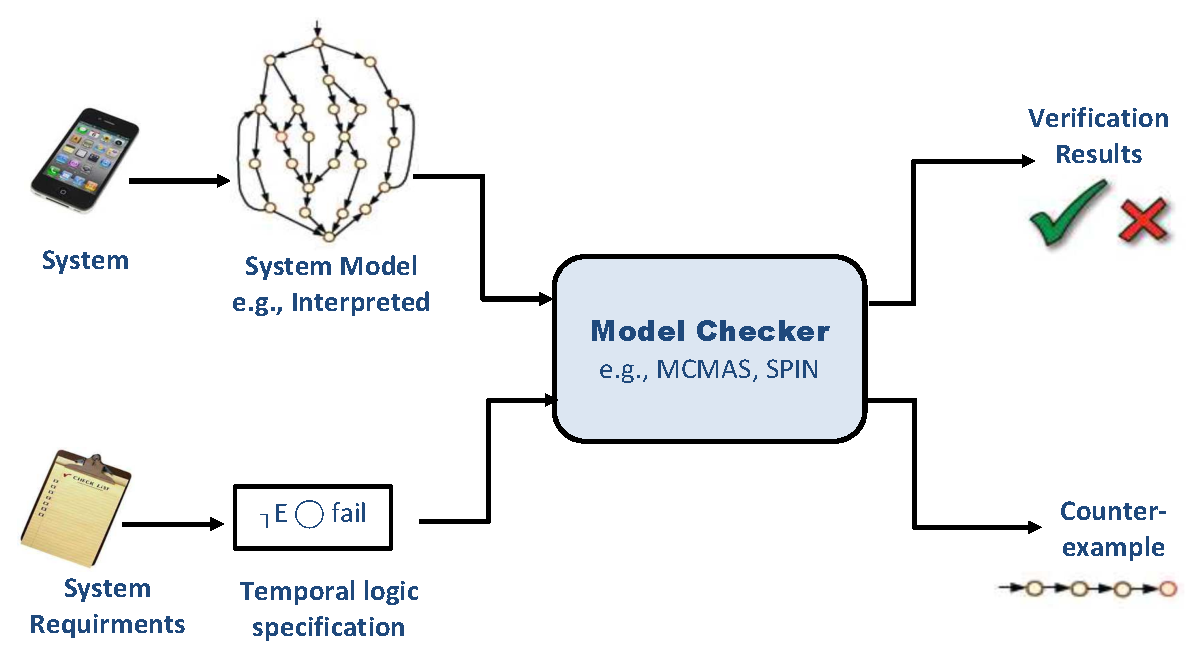
\includegraphics[width=12cm, height=7cm]{chap2/img/modelchecking1.eps}
                \end{center}
                \caption{Qualitative model checking overview}
                \label{fig:model-checking-cha2}
                \end{figure}

\subsection{Probabilistic Model Checking} \label{sec:pro-Model-Checking-cha2}

In addition to qualitative model checking, quantitative (or probabilistic) model checking techniques based on probabilistic model checkers have recently gained popularity \cite{Baier2008}. Probabilistic model checking is an automatic formal verification technique for the analysis of systems exhibiting stochastic behavior \cite{Hinton2006}. It offers the capability for interpreting the satisfiability of a given property in terms of quantitative results. In fact, the probabilistic model checking technique is similar to conventional model checking as discussed earlier. The major difference is that a probabilistic model contains additional information on the likelihood of transitions between states, or to be more specific, it can model probabilistic behavior. An overview of the probabilistic model checking procedure is given in Figure \ref{fig:prob-model-checking-cha2}. It shows that a probabilistic model checker takes as input a property and a model and delivers the result ``Yes'' or ``No'', or some probability.


\begin{figure}[t]
                \begin{center}
                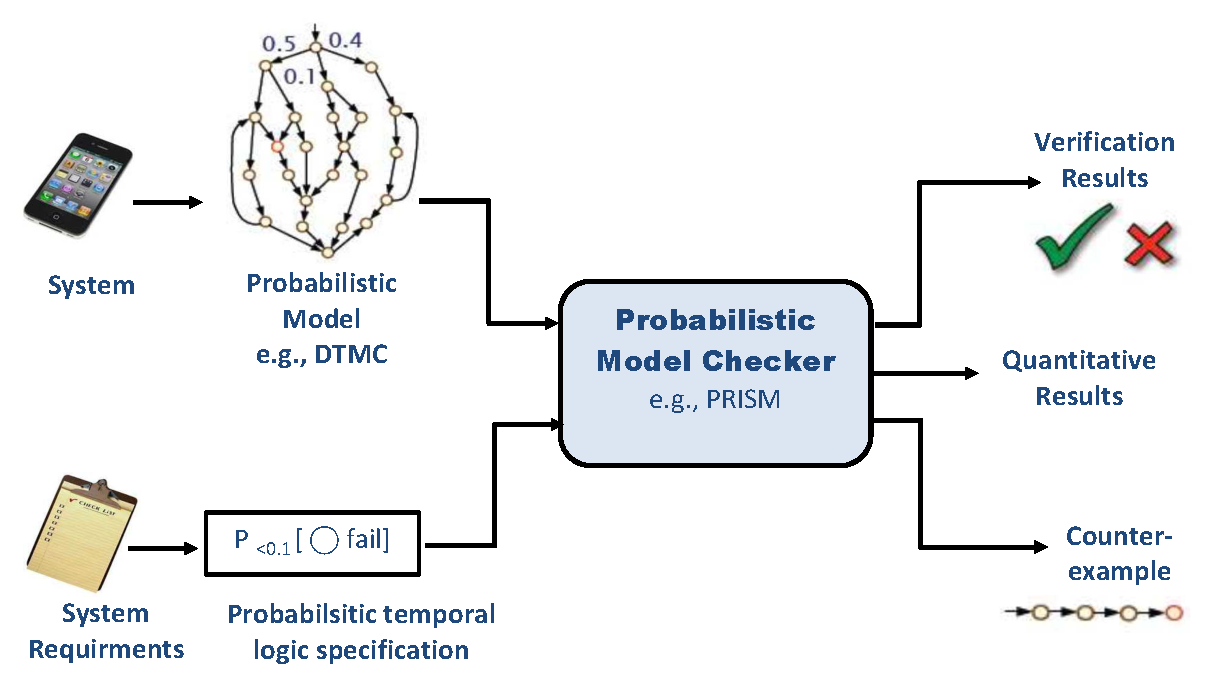
\includegraphics[width=12cm, height=7cm]{chap2/img/modelchecking2.eps}
                \end{center}
                \caption{Probabilistic model checking overview}
                \label{fig:prob-model-checking-cha2}
                \end{figure}


\subsection{Model Checking Tools}
There have been various model checking tools (also known as Model Checkers) in the literature. In this section, we review some of the most widely used model checkers.
\begin{itemize}

\item \textbf{MCMAS}\\
    MCMAS (Model Checker for Multi-Agent Systems) \cite{Lomuscio2006} is an OBDD-based symbolic model checker developed for the purpose of verifying epistemic properties of multi-agent systems. It supports branching-time temporal logic CTL. It also supports interpreted systems as an underling formalism for modeling target systems. The dedicated programming language used for describing a MAS in MCMAS is called ISPL (Interpreted Systems Programming Language). MCMAS was originally designed to handle the logic of knowledge CTLK and the branching-time temporal logic CTL. Recently, it has been extended by implementing some new algorithms that allow it to accept commitment formulae and hence to verify social commitments. The new extended version is called MCMASC (MCMAS for commitments). \cite{El-Menshawy2012}.


\item \textbf{NuSMV}\\
    NuSMV \cite{Cimatti2002}, an extension version of SMV \cite{McMillan1992}, is a well-known and widely trusted model checker. It is written in ANSI C language. As an input language, NuSMV accepts files written in SMV language. While the SMV tool was originally developed to implement the OBDD-based symbolic model checking for CTL, NuSMV implements also bounded model checking techniques for LTL -- in addition to the symbolic model checking techniques for CTL. This feature distinguishes it the most from SMV. Nevertheless, both SMV and NuSMV allow for a compact description of systems under consideration using modules, which may be composed to describe the evolution of states.



\item \textbf{SPIN}\\
    The SPIN \cite{Holzmann1997} model checker is one of the most used tools for tracing software defects in concurrent system designs. It was introduced in the 1980s at Bell Labs. Later, it has been made available to the public. The original version of SPIN has been continually under development and improvement. SPIN's programming language is called PROMELA. \cite{Holzmann2003} details the theoretical foundations of SPIN and presents the user manual. The main characteristics of SPIN are:

    $\diamond$ It is designed for the temporal logic LTL.\\
    $\diamond$ It is an automata-based model checker.\\
    $\diamond$ It implements various optimization strategies, including on-the-fly model checking and partial order reduction.

\item \textbf{PRISM} \\
    PRISM \cite{Kwiatkowska2002} stands for Probabilistic Symbolic Model Checker. It is the leading tool in the area of probabilistic model checking. The tool is widely used for checking probabilistic specifications over probabilistic models. The specifications can be expressed either in PCTL or in Continuous Stochastic Logic (CSL) \cite{Baier2008,Forejt2011}. Systems models can be described using the PRISM language as Discrete-Time Markov Chains (DTMCs), Continuous-Time Markov Chains (CTMCs), or Markov Decision Processes (MDPs). PRISM has been successfully used to analyse systems with a wide range of application domains, including communication and multimedia protocols, randomised distributed algorithms, security protocols, and many others.
    PRISM is the most appropriate tool for our work thanks to its capability of verifying probabilistic properties, and accepting formulae written in PCTL. Using PRISM, it is possible to either determine if a probability satisfies a given bound or obtain the actual value.

\item \textbf{MCK} \\
    MCK (stands for Model Checking Knowledge) is a model checker for the logic of knowledge, developed at the School of Computer Science and Engineering at the University of New South Wales \cite{Gammie2004}. It is implemented using OBDD-based symbolic algorithms. In the epistemic dimension, agents may use their observations in a variety of ways to determine what they know: observation alone, observation and clock, and perfect recall of all observations. The former way (observation alone) is to evaluate an agent's knowledge based merely on its current observation. The second way (observation and clock) is to compute an agent's knowledge based both on its current observation and the current clock value. The latter way (perfect recall of all observations) is to compute an agent's knowledge based on the complete record of all its observations.

    In the temporal dimension, specification formulae may use either linear time temporal logic (LTL), or the branching-time logic (CTL).
    Recently, MCK was extended by Huang et al. \cite{Huang2011} to permit the verification of knowledge in the presence of probabilistic behavior.





\end{itemize}

\section{Summary}\label{sec:summary-chap2}
In this chapter, we introduced the background and concepts needed for the rest of my thesis. As social commitments are the main focus of this research, it is important, again, to emphasis that the notion of ``social commitments'' we consider in this thesis is the communicative social commitments that are public and observable. In the next chapter, we propose a new probabilistic approach for handling social commitments in the presence of uncertainty.


%%%%%%%%%%%%%%%%%%%%%%%%%%%%%%%%%%%%%%%%%%%%%%%%%%%%%%%%%%%%%%%%%%%%%%%%%%%%%%%
%% Chapter 3 : Probabilistic Social Commitments.
%%%%%%%%%%%%%%%%%%%%%%%%%%%%%%%%%%%%%%%%%%%%%%%%%%%%%%%%%%%%%%%%%%%%%%%%%%%%%%%
\setcounter{chapter}{2}


\chapter{Coalition Formation for Autonomous Web Services}\label{sec:coalitionformationws}

In this chapter, we present our coalition model of agent-based web
services within communities \cite{SCC2013efficient}. We start by describing the general
architecture and considered parameters for web services.
Thereafter, problem modeling and formulation will be introduced in
terms of task distribution and community revenue. Web service
cooperative games in different settings will follow along with
some simulation results.

\section{Preliminaries}\label{s:preliminaries}

In this section, we discuss the parameters and preliminary
concepts that we use in the rest of the chapter.

\subsection{Architecture}

Our system consists of three main types of entities working
together:

\emph{1) Web services} are rational entities that aim to maximize
their utilities by providing high quality services to end users.
They aim to maximize their individual income by receiving enough
requests from end users. In order to increase their revenue, web
services seek for more tasks if they have the capacity and
throughput to do so. Web services can join communities to have
better efficiency by collaborating with others, to have access to
higher market share, and to have opportunity of receiving a bigger
task pool from end users. Throughout this thesis, in our
equations, we refer to web services as $ws$ and to the set of web
services hosted by a given community as $C$. To simplify the
notation, sometimes we simply write $ws$ instead of $ws \in C$ to
go through the elements $ws$ of the set $C$.

\emph{2) Master Web Services} or the community coordinators, are representatives of the
communities of web services and responsible for their management.
Communities receive requests from users and aim to host a healthy
set of web services to perform the required tasks. They seek to
maximize user satisfaction by having tasks accomplished according
to the desired QoS. In fact, higher user satisfaction will bring
more user requests and increase the market share and revenue of
the community.

\emph{3) Users} generate requests and try to find the best
available services. User satisfaction is abstracted as function of
quantity and quality of tasks accomplished by a given service.
Higher user satisfaction leads to higher trust of the community by users hence directing more requests towards that service provider.

\subsection{Web Service Parameters}\label{ws_parameters}

Web services come with different quality of service parameters.
These parameters with a short description are listed in Table
\ref{qosws}.

\begin{table}[!t]
\centering
\caption{List of web service QoS parameters.}
\begin{tabular}{|c|c||c|c|}
\hline
\textbf{Parameter} & \textbf{Definition} \\
\hline\hline
$Availability$ & Probability of being available during \\
&a time frame \\
$Reliability$ & Probability of successfully handling \\
&requests during a timeframe\\
$Successability$ & Rate of successfully handled requests \\
$Throughput$ & Average rate of handling requests \\
$Latency$ & The average latency of services\\
$Capacity$ & Amount of resources available\\
$Cost$ & Mean service fee \\
$Regulatory$ & Compliance with standards, law and rules\\
$Security$ & Quality of confidentiality \\
&and non-repudiation\\
\hline
\end{tabular}
\label{qosws}
\end{table}


We adopted a real world dataset \cite{DBLP:conf/smc/Al-MasriM09a}
which has aggregated and normalized each of these parameters to a
real value between 0 and 1. Since requests are not shared among
web services and are distributed among all of them inside a
community, each one of them comes with a given QoS denoted by
$(QoS_{ws})$. We assume that $(QoS_{ws})$ is obtained by a certain
aggregation function of the parameters considered in Table
\ref{qosws}. We use this quality output later in evaluating the
community \emph{worth} or \emph{payoff} function.

\subsection{Web Service Communities}\label{webservice-communities}

Figure 3 represents our revised architecture of web service
communities where tasks are to be distributed among the members
that are interested in forming stable coalitions. As discussed in
Chapter 2, communities are essentially virtual platforms
aggregating web services having similar and complementary
functionalities and communicate with other entities such as UDDI
registries and users using particular protocols. Web services join
communities to increase their utility by having larger market
share and task pool. Community coordinators or master web services
are responsible for community development, managing membership
requests from web services and distributing user tasks among the
community members. Community coordinators try to attract quality
web services and keep the community as stable and productive as
possible to gain better reputation and user satisfaction, which
results in having higher revenue.

\begin{figure*}[!t]
\centerline{\includegraphics[width=15cm]{Figures/archss.eps}}
\caption{Architecture of Web Service communities}
\label{fig_community}
\end{figure*}


\section{Problem Formulation and Modeling}\label{s:model}

In this section, we present  web services and community coordinator's interactions, the task distribution process and revenue models in web service communities.

\subsection{Task Distribution}

As mentioned in Section \ref{s:preliminaries}, communities
are robust service providers with well established market share
and reputation. By maintaining their reputation and performance,
they attract  end users which choose them as service providers to
perform their tasks. The community master is characterized by a
request rate $(R_C)$ from users. Each web service comes with a
given QoS ($QoS_{ws}$) from which the throughput $Th_{ws}$ is
excluded. Throughput is the average rate of tasks a web service
can perform per time unit. Its exclusion from $QoS_{ws}$ allows us
to build our analysis on the particular value of $Th_{ws}$. Thus,
web services perform tasks with an average output quality of
$QoS_{ws}$ and a throughput rate of $Th_{ws}$.

The community master uses a slightly modified \emph{weighted fair queuing} method to distribute tasks among its members. The goal is to allocate incoming tasks to web services with a rate matching the throughput value of $Th_{ws}$. In \emph{weighted fair queuing} method \emph{all} the input flow is multiplexed along different paths, however in our case if the input rate $(R_C)$ of the community is more than the summation of throughput values of the web services in the community, some of the input tasks will be queued and served with delay. Thus, the amount of tasks performed by community is $\sum_{ws \in C}{(Th_{ws})}$ when $\sum_{ws}{Th_{ws}} \leq R_{C}$. However, when the input rate $(R_C)$ of the community is less than the summation of throughput values of the web services in the community,
%the community has more web services having more total throughput value than community's request rate
$(R_C)$ the \emph{weighted fair queuing} algorithm assigns a weighted task rate of $R_C \times \frac{Th_{ws}}{\sum_{ws}{Th_{ws}}}$ for each web service ($ws$) and the total rate of tasks being performed is $R_C$, the community's receiving request rate.

While distributing tasks, the community master can verify the performance, throughput and quality of service of   tasks being performed by web services. It can recognize if web services are capable of doing the amount of tasks they advertised. If for any reason there is a decline in quality metrics or throughput, the  community master will announce the new parameters and community masters and members can consider those values as benchmark for future performance calculations.
Web services that got their quality declined are penalized, and in this way, players have incentive to reveal their real capabilities to profit best from the community and to avoid being penalized. In addition, the system should be dynamic enough to detect and react to web services quality metrics variation as over time web service metrics may  degrade or improve, a change that the community should adjust to.
% Therefore its easy for the system to encourage players to be in some sense incentive compatible in the way that they would profit best by truthfully revealing their capabilities. Also it is important to be dynamic enough to consider web services which may have their quality metrics degraded or even improved over time for any reason and be able to adjust the community with new parameters.


\subsection{Community Revenue}

The communities and web services earn revenue by performing tasks.
The total gain is function of quality ($QoS_{ws}$) and throughput
($Th_{ws}$) of tasks being performed. We have adopted a linear equal weight average over
the QoS parameters excluding the
$Throughput$ and $Cost$ parameters. A community has the option to
weigh specific QoS parameters depending on the expectations of
their clients.

The maximum potential output of a community $(PO(C))$  is an aggregation of number of tasks, times their quality, for each web service member of the community:

\begin{equation}
PO(C) = \sum_{ws \in C}{(T_{ws} \times QoS_{ws})}
\end{equation}

If the summation of throughput values ($Th_{ws}$) of community members exceeds the input task rate of the community ($R_C$) the community cannot perform at its maximum potential. It denotes the case when the community has more web services than it needs to perform the input task load. The actual output has to be normalized to the amount of tasks being performed.

\begin{equation}\label{out_c}
Out(C) = \left\{
  \begin{array}{l l}
    PO(C) & \quad \text{if $\sum_{ws}{Th_{ws}} \leq R_{C}$}\\
    PO(C) \times \frac{R_{C}}{\sum_{ws}{Th_{ws}}} & \quad \text{if $\sum_{ws}{Th_{ws}} > R_{C}$}
  \end{array} \right.
\end{equation}

The revenue function of the web service community is a linear function of $Out(C)$ with a positive constant multiplier.

\subsection{Case Study}

In this section, we analyze three numerical examples and discuss the motivation of web services and community interactions and the strategies they can adopt and the revenue they can earn adopting these different strategies.


%%%%%%%%%%%%%%%%%%%%%%%%% EXAMPLE 1 %%%%%%%%%%%%%%%%%%%%%%%%%%%%%%%%%%%%
\begin{table}[!t]
\renewcommand{\arraystretch}{1.3}
% if using array.sty, it might be a good idea to tweak the value of
% \extrarowheight as needed to properly center the text within the cells
\caption{Case Study: Example 1}
\label{example_1}
\centering
\begin{tabular}{c c c c}
\hline
$WS$ & $QoS_{ws}$ & $Th_{ws}$ & $Th_{ws} \times QoS_{ws}$\\
\hline
1 & 0.8 & 4 & 3.2\\
2 & 0.8 & 5 & 4.0\\
3 & 0.8 & 3 & 2.4\\
\hline
\end{tabular}
\end{table}

\begin{table}[!t]
\renewcommand{\arraystretch}{1.3}
% if using array.sty, it might be a good idea to tweak the value of
% \extrarowheight as needed to properly center the text within the cells
% \caption{Three web services}
\label{example_1_2}
\centering
\begin{tabular}{c c || c c}
\hline
Community & Worth & Community & Worth\\
\hline
$\left\{1\right\}$ & 3.2 & $\left\{1,2\right\}$ & 7.2\\
$\left\{2\right\}$ & 4.0 & $\left\{1,3\right\}$ & 5.6\\
$\left\{3\right\}$ & 2.4 & $\left\{2,3\right\}$ & 6.4\\
$\left\{1,2,3\right\}$ & 8.0\\
\hline
Community $R_C$: 10\\
\hline
\end{tabular}
\end{table}
%%%%%%%%%%%%%%%%%%%%%%%%% EXAMPLE 1 %%%%%%%%%%%%%%%%%%%%%%%%%%%%%%%%%%%%

%%%%%%%%%%%%%%%%%%%%%%%%% EXAMPLE 2 %%%%%%%%%%%%%%%%%%%%%%%%%%%%%%%%%%%%
\begin{table}[!t]
\renewcommand{\arraystretch}{1.3}
% if using array.sty, it might be a good idea to tweak the value of
% \extrarowheight as needed to properly center the text within the cells
\caption{Case Study: Example 2}
\label{example_2}
\centering
\begin{tabular}{c c c c}
\hline
$WS$ & $QoS_{ws}$ & $Th_{ws}$ & $Th_{ws} \times QoS_{ws}$\\
\hline
1 & 0.8 & 5 & 4.0\\
2 & 0.7 & 6 & 4.2\\
3 & 0.7 & 4 & 2.8\\
\hline
\end{tabular}
\end{table}

\begin{table}[!t]
\renewcommand{\arraystretch}{1.3}
% if using array.sty, it might be a good idea to tweak the value of
% \extrarowheight as needed to properly center the text within the cells
% \caption{Three web services}
\label{example_2_2}
\centering
\begin{tabular}{c c || c c}
\hline
Community & Worth & Community & Worth\\
\hline
$\left\{1\right\}$ & 4.0 & $\left\{1,2\right\}$ & 7.4\\
$\left\{2\right\}$ & 4.2 & $\left\{1,3\right\}$ & 6.8\\
$\left\{3\right\}$ & 2.8 & $\left\{2,3\right\}$ & 7.0\\
$\left\{1,2,3\right\}$ & 7.3\\
\hline
Community $R_C$: 10\\
\hline
\end{tabular}
\end{table}
%%%%%%%%%%%%%%%%%%%%%%%%% EXAMPLE 2 %%%%%%%%%%%%%%, %%%%%%%%%%%%%%%%%%%%%%

In the first example,  we present the case of a community with
$R_C =10 $, and three web services, each having different
$QoS_{ws}$ and $Th_{ws}$ values as listed in Table
\ref{example_1}. The worth of a community is calculated based on
$Out(C)$ equation (\ref{out_c}) which is the amount of output
being generated by the community. The first table  lists the web
services with their aggregated $QoS_{ws}$ parameters, their task
input rate while working alone, and also their  throughput value
$Th_{ws}$. The second table shows all the possible communities and
their respective worth. The obtained values suggest that
communities having more web services have better gain and output.
However each community needs to  distribute the gain between web
services. Sometimes it is impossible to share the gain between all
web services in a way that no subset of them would individually
gain more if they form their own group. In this example, the value
community of ${ws_1}$ and ${ws_2}$ is 7.2, With ${ws_3}$ joining
the community the worth increases to 8.0. However there is no way
to distribute the value among web services to have  ${ws_1}$ and
${ws_2}$  earning 7.2, and ${ws_3}$ earning at least 2.4, the gain
they could earn before joining the community. This fact makes the
group unstable. In the second  example, shown in Table
\ref{example_2}, we even have situations where a web service
(${ws_3}$) joining a community ($\left\{ws_1,ws_2\right\}$)
decreases the value of community. The reason is, the community is
already full and all tasks are almost being distributed and new
community with bad quality can degrade the average quality of
tasks being done by the community. In both examples, the request
of joining of web service ${ws_3}$ should be rejected by the
community.

%%%%%%%%%%%%%%%%%%%%%%%%% EXAMPLE 3 %%%%%%%%%%%%%%%%%%%%%%%%%%%%%%%%%%%%
\begin{table}[!t]
\renewcommand{\arraystretch}{1.3}
% if using array.sty, it might be a good idea to tweak the value of
% \extrarowheight as needed to properly center the text within the cells
\caption{Case Study: Example 3}
\label{example_3}
\centering
\begin{tabular}{c c c c}
\hline
$WS$ & $QoS_{ws}$ & $Th_{ws}$ & $\text{\emph{Input Task Rate}}$\\
\hline
1 & 0.8 & 10 & 5\\
2 & 0.8 & 20 & 5\\
3 & 0.8 & 30 & 5\\
\hline
\end{tabular}
\end{table}

\begin{table}[!t]
\renewcommand{\arraystretch}{1.3}
% if using array.sty, it might be a good idea to tweak the value of
% \extrarowheight as needed to properly center the text within the cells
% \caption{Three web services}
\label{example_3_2}
\centering
\begin{tabular}{c c || c c}
\hline
Community & Worth & Community & Worth\\
\hline
$\left\{C_{ms_1}\right\}$ & 0 & $\left\{C_{ms_2}\right\}$ & 0\\
$\left\{C_{ms_1}, ws_1\right\}$ & 8 & $\left\{C_{ms_2}, ws_1\right\}$ & 8\\
$\left\{C_{ms_1}, ws_2\right\}$ & 16 & $\left\{C_{ms_2}, ws_2\right\}$ & 16\\
$\left\{C_{ms_1}, ws_3\right\}$ & 16 & $\left\{C_{ms_2}, ws_3\right\}$ & 24\\
$\left\{C_{ms_1}, ws_1, ws_2\right\}$ & 16 & $\left\{C_{ms_2}, ws_1, ws_2\right\}$ & 24\\
$\left\{C_{ms_1}, ws_1, ws_3\right\}$ & 16 & $\left\{C_{ms_2}, ws_1, ws_3\right\}$ & 32\\
$\left\{C_{ms_1}, ws_2, ws_3\right\}$ & 16 & $\left\{C_{ms_2}, ws_2, ws_3\right\}$ & 32\\
$\left\{C_{ms_1}, ws_1, ws_2, ws_3\right\}$ & 16 & $\left\{C_{ms_2}, ws_1, ws_2, ws_3\right\}$ & 32\\
$\left\{C_{ms_1}, C_{ms_2}, ...\right\}$ & 0 & $\left\{ws_1\right\}$ & 6.8\\
$\left\{ws_2\right\}$ & 4.2 & $\left\{ws_3\right\}$ & 6.8\\
\hline
Community $R_{C_1}$: 20 \\ Community $R_{C_2}$: 40\\
\hline
\end{tabular}
\end{table}
%%%%%%%%%%%%%%%%%%%%%%%%% EXAMPLE 3 %%%%%%%%%%%%%%%%%%%%%%%%%%%%%%%%%%%%

In Example 3, we consider the case of having different communities with different market share, ${R_C}$ values. Web services also have a small share of market independently, providing them with a small task pull. In these kind of scenarios, the solution considers individual maximization of payoff and also the total worth of all communities which represents the \emph{social welfare}. In this example the most efficient partition of web services is earned by having two coalitions of $\left\{C_{master_1}, ws_2\right\}$ and $\left\{C_{master_2}, ws_1, ws_3\right\}$, which yields a total value of $32 + 16 = 48$. In these types of scenarios, the goal is to reach stability, adopting a distributed approach where all players have the power of choice on the decision of whether or not they join a coalition. The communities usually start the game having some established members, encountering new web services, the communities may exchange web services and new web services would join them having at least one player gaining utility, without hurting any other participant. In this example if we initially having two coalitions of $\left\{C_{master_1}, ws_2\right\}$ and $\left\{C_{master_2}, ws_1\right\}$ and a ${ws_3}$ as new web service, ${ws_3}$ joining ${C_{master_1}}$ would hurt at least itself or $ws_2$, however ${ws_3}$ joining ${C_{master_2}}$ would not hurt any participants and ${ws_3}$ would earn more within the community and the community will have enough web services performing the incoming tasks from users.

The first two examples illustrate the fact that a community cannot simply increase its revenue by adding more web services. The web services and even community owners are autonomous agents and would deviate and be displeased about the community if new members cause a drop in their profit. The job of the community master is to attract as many quality web services it can and keep them satisfied; hence the group stability is guaranteed.
The third example highlights another type of problem we would like to address, which is how to form best possible groups of communities, and allocate web services among communities in a way which would maximize payoff for of our agents and members already residing in the communities.
In next section, we provide collaborative game theory based algorithms for our autonomous agents, to tackle these problems and find applicable and efficient strategies for communities and web services to maximize their profit.

 \section{Web Service Cooperative Games}\label{s:game_solution}

In this section, we present different web service community models
and focus on the problem of how both web services and community
masters as rational entities would adopt strategies to maximize
their payoff.

\subsection {Web Services and One Community}

In this scenario, we assume the existence of a typical community
managed by its master, and web services need to join it to be able
to get requests from the master. The community master is
characterized by a requests rate $(R_{C})$ from users. Each web
service comes with a given QoS ($QoS_{ws}$). The worth of a community
$v(C)$ is set to Out(C) based on equation \ref{out_c}.

As mentioned in previous section, the worth and output of a
community  is a function of the
throughput and provided QoS of its web service members. If the throughput rate is more than
the master's input request rate, it means the web services inside
the community are capable of serving more requests than the
demand. Considering this factor, the valuation function is
designed to balance the output performance so that it matches the
exact throughput rate and QoS the web service can provide within
the particular community.
%** In the case where the limited tasks are distributed among web services uniformly, the value of coalition would be the proportion of the average QoS times their throughput to rate of available requests. **

In this first scenario, we only consider one grand coalition and
analyze the system from the point of view of one single master web
service and a collection of web services. The master web service
decides which members can join
%or should leave%
the community and distributes the requests and income among its
community members (see Figure \ref{fig_sim1}).

\begin{figure}[!t]
\centering
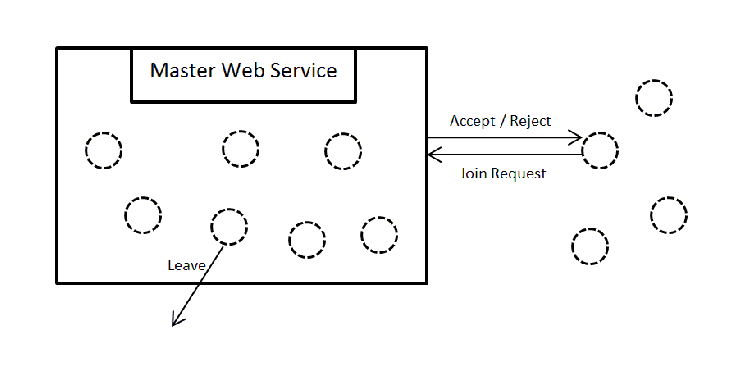
\includegraphics[width=3in]{Figures/s1.eps}`
\caption{Web Services and A Grand Community}
\label{fig_sim1}
\end{figure}

The membership decision is made based on throughput and \emph{QoS}
of the considered web service. The goal is to have quality web
services in the community so it stays stable and no other web
services would have incentives to deviate and leave the coalition
$C$. Therefore, a basic method would be to check the core of the
coalition $C$ considering all the current community members (all
web services already residing within the community) and the new
web service. This algorithm uses the \emph{Shapley value}
distribution method as described in Equation \ref{eq:shapley} to
distribute the gain of $v(C)$ among all the members and then
checks if the \emph{Shapley value} payoff vector for this
community having the characteristic function $v(C)$ is in the
\emph{core}. In the \emph{Shapley value} payoff vector, the payoff
for each web service $ws_i$ is calculated based on its marginal
contribution $v(C \cup {i}) - v(C)$ over all the possible
different permutations in which the coalition can be formed, which
makes the payoff distribution fair. Because of going through all
the possible permutations of subsets of $N$, the nature of the
\emph{Shapley value} is combinatorial, which makes it impractical
to use as the size of our coalitions grows. However, it is proven
that in convex games, the \emph{Shapley value} lies in the core
\cite{DBLP:conf/ijcai/GrecoMPS11, myerson1991game}. Thus, if the
\emph{Core} is non-empty, the payoff vector is a member of the
\emph{Core}. The following proposition is important to make our
algorithm tractable.
% so in our algorithm we check the core membership of this payoff vector.

%\ref{eq:convex}.

%\newtheorem{theorem}{Proposition}
%\begin{theorem}[Einstein-Podolsky-Rosenberg]
\begin{theorem}\label{proposition1}
A game with a characteristic function $v$
is convex if and only if for all $S$, $T$, and $i$ where $S
\subseteq T \subseteq N \backslash \left\{i\right\}, \forall i \in
N$,
%For $\forall S \subseteq T \subseteq N \backslash \left\{i\right\}, \forall i \in N$ we have:
\begin{equation}\label{eq:convex_snow}
v(S \cup \left\{i\right\}) - v(S) \leq v (T \cup \left\{i\right\}) - v(T)
\end{equation}
\end{theorem}

%\begin{Proposition}\label{proposition} A game with a characteristic function $v$
%is convex if and only if for all $S$, $T$, and $i$ where $S
%\subseteq T \subseteq N \backslash \left\{i\right\}, \forall i \in
%N$,
%For $\forall S \subseteq T \subseteq N \backslash \left\{i\right\}, \forall i \in N$ we have:
%\begin{equation}\label{eq:convex_snow}
%v(S \cup \left\{i\right\}) - v(S) \leq v (T \cup \left\{i\right\}) - v(T)
%\end{equation}
%\end{Proposition}

\begin{proof}
We first prove the ``only if'' direction:
%\\$~~~~$\textbf{1}. ``only if'' direction:\\
\\$~~~~$\ \textbf{1}. ``only if'' direction:\\
%\setlength{\abovedisplayshortskip}{2pt}
Assume:\\
\vspace{-0.5cm}
\begin{gather*}\label{convexsnowproof}
v(S \cup \left\{i\right\}) - v(S) \leq v (T \cup \left\{i\right\})
- v(T)
\\
\rightarrow v(S \cup \left\{i\right\}) + v(T) \leq v (T \cup \left\{i\right\}) + v(S)
\end{gather*}

Considering $S \subseteq T$:
\setlength{\abovedisplayshortskip}{2pt}
\begin{gather*}
T \cup \left\{i\right\} = (S \cup \left\{i\right\}) \cup T
\\
S = (S \cup \left\{i\right\}) \cap T
\end{gather*}

By setting $A = S \cup \left\{i\right\}$ and $B = T$ we have:
\setlength{\abovedisplayshortskip}{2pt}
\begin{gather*}
v(S \cup \left\{i\right\}) + v(T) \leq v (T \cup \left\{i\right\}) + v(S)
\\
\rightarrow v(S \cup \left\{i\right\}) + v(T) \leq
\\
v((S \cup \left\{i\right\}) \cup T) + v((S \cup \left\{i\right\}) \cap T)
\\
\rightarrow v(A) + v(B) \leq v(A \cup B) + v(A \cap B)
\end{gather*}
Consequently, the game is convex.

\textbf{2}. ``if'' direction:\\
Assume the game is convex. Thus, for all $A, B \subset N$, we
have: \setlength{\abovedisplayshortskip}{2pt}
\begin{gather*}
v(A) - v(A \cap B) \leq v(A \cup B) - v(B)
\end{gather*}

By setting $S \cup \left\{i\right\} = A$ and $T = B$ where $S \subseteq T$:
\setlength{\abovedisplayshortskip}{2pt}
\begin{gather*}
v(S \cup \left\{i\right\}) - v((S \cup \left\{i\right\}) \cap T) \leq v(T \cup (S \cup \left\{i\right\})) - v(T)
\\
\rightarrow v(S \cup \left\{i\right\}) - v(S) \leq v(T \cup \left\{i\right\}) - v(T)
\end{gather*}

\end{proof}

Thus, in order to keep the characteristic function convex, new web
services should have more marginal contribution as the coalition
size grows.

Our algorithm works as follows. Given an  established community
with a master and some member web services, a web service would send a \emph{join request} to join  the
community. Ideally, the \emph{core}
or \emph{$\epsilon$-core} stability of the group having this new
member should be analyzed. As the normal core membership algorithm is computationally
intractable, we exploit Proposition \ref{proposition1} and Equation
\ref{eq:convex_snow} to check the convexity of our game having
characteristic function where the new member is added. In the
equation, let $C$  be our community members before
having the new web service join the community. Let  ${i}$ be the new web
service, and then verify the equation for $S$, setting $ S = T /
W1 $ where $W1$ is the set of all possible subsets of the set $N$
having the size $1$. We can relax the equation a bit by adding a
constant $\epsilon$ to the left side of the equation. We call this
method \emph{Depth-1 Convex-Checker} algorithm. If the equation is
satisfied for all $W1$, we let the new web service join our
community, since the web service will contribute positively enough
to make our new community stable. Since only subsets of size $1$
are checked, the following Proposition holds.

\begin{theorem}\label{complexity1}
\emph{The run time complexity of Depth-1 Convex-Checker algorithm is
$O(n)$.}
\end{theorem}

By this result, we obtain a significant reduction from $O(2^n)$,
which is the complexity of checking all possible subsets of $N$.
In our second method, we use the same algorithm, but this time we
set $W2$ to be the set of all possible subsets of size two and one
of the community $C$. We call this method \emph{Depth-2
Convex-Checker} and its run time complexity is still
linear:

\begin{theorem}\label{complexity2}
\emph{The run time complexity of Depth-2 Convex-Checker algorithm is
$O(n^2)$.}
\end{theorem}

It is possible to develop an algorithm that continues the
verification of this condition against subsets of size $3$,
$4$, etc. until the algorithm gets interrupted.

\subsection {Web Services and Many Communities}

In this scenario, we consider multiple communities managed by
multiple master web services, each of which is providing
independent request pools (see Figure \ref{fig_sim2}). Identical
to the first scenario, master web services form coalitions with
web services. We use coalition structure formation methods to
partition web services into non-empty disjoint coalition
structures. As mentioned in Section \ref{sec:coalition}, the used
algorithms in \cite{Sandholm:1999:CSG:317145.317152,DBLP:conf/ijcai/GrecoMPS11,DBLP:conf/ijcai/RahwanMJ11} try to
solve key fundamental problems of what coalitions to form, and how
to divide the payoffs among the collaborators.

\begin{figure}[!t]
\centering
\includegraphics[width=3in]{Figures/s2.eps}
\caption{Web Services and Many Communities}
\label{fig_sim2}
\end{figure}

In coalition-formation games, formation of the coalitions is the
most important aspect. The solutions focus on maximizing the
social welfare. For any coalition structure $\pi$, let
$v_{cs}(\pi)$ denote the total worth $\sum_{C \in \pi}{v(C)}$,
which represents the \emph{social welfare}. The solution concepts
in this area deal with finding the maximum value for the social
welfare over all the possible coalition structures $\pi$. There
are $centralized$ algorithms for this end, but these approaches
are generally NP-complete. The reason is that the number of all
possible partitions of the set $N$ grows exponentially with the
number of players in $N$, and the centralized algorithms need to
iterate through all these partitions.
%These algorithms \cite{DBLP:conf/ijcai/GrecoMPS11, DBLP:conf/ijcai/RahwanMJ11, RePEc:wpa:wuwpga:0110001} are centralized algorithms, where all the complexity. However these algorithms are more intractable than Core stable solutions and practical with some constraints in practice\cite{RePEc:wpa:wuwpga:0110001}.
In our model, we propose using a distributed algorithm where each
community master and web service can be a decision maker and
decide for its own good. The aim is to find less complex and
distributed algorithms for forming web services coalitions
\cite{DBLP:journals/igtr/AptW09,Dieckmann02dynamiccoalition,ray2007game}.
The distributed merge-and-split algorithm in
\cite{DBLP:journals/igtr/AptW09} suits our application very well.
It keeps splitting and merging coalitions to partitions which are
preferred by all the players inside those coalitions.

This merge-and-split algorithm is designed to be adaptable to
different applications. One major ingredient to use such an
algorithm is a preference relation or well-defined orders proper
for comparing collections of different coalition partitions of the
same set of players. Having two partition sets of players, namely
$P = {P_1,...,P_k}$ and $Q = {Q_1,...Q_l}$, one example would be
to use the social welfare comparison $\sum^k_{i=1}v(P_i) >
\sum^l_{j=1}v(Q_j)$. For our scenario, we use \emph{Pareto order}
comparison, which is an individual-value order appropriate for our
self-interest web services. In the Pareto order, an allocation or
partition $P$ is preferred over another $Q$ if at least one player
improves its payoff in the new allocation and all the other
players still maintain their payoff ($p_i \geq q_i$ with at least
one element $p_i > q_i$).

The valuation function $v(C)$ for this scenario is the same as
\emph{``Web Services and One Community''} scenario. However, in
order to prevent master web services joining the same community,
we set $v(C) = 0$ when $C$ has either none, or more than one
master web service as member.

In this scenario, as new web services are discovered and get ready
to join communities, our algorithm keeps merging and splitting
partitions based on the preference function. The decision to merge
or split is based on the fact that all players must benefit. The
new web services will merge with communities if $all$ the players
are able to improve their individual payoff, and some web services
may split from old communities, if splitting does not decrease the
payoff of \emph{any} web service of the community. According to
\cite{DBLP:journals/corr/abs-cs-0605132}, this sequence of merging
and splitting will converge to a final partition, where web
services cannot improve their payoff. More details of this
algorithm and analysis of generic solutions on coalition formation
games are described in \cite{DBLP:journals/igtr/AptW09}.

\subsection{Taxation, Subsiding and Community Stability}\label{s:tax}

We discussed $core$ as one of the prominent solution concepts in
cooperative games. Working together, completing tasks and
generating revenue, agents need to distribute the gain in a way no
agents would gain more by forming their own group. However, in
most cases, the core of a game is empty, so we introduced the
\emph{$\epsilon$-core} concept, where agents would only earn a
minimal amount of $\epsilon$ by deviating from the coalition.
Stability is an attractive property for communities. In addition,
communities would benefit by having slightly more web services
than the exact number of web services needed to satisfy the task
rate cap. This is because there is always a possibility that the
web services may leave the community or they may under perform and
degrade the quality values they were initially performing with.

The solution we propose for communities to ensure stability is
applying a tax $\epsilon$, which is an amount of cost for those
web services that decide to change communities (let us say from
$C$ to $C'$), which would make deviation a costly act. However,
this would require all the community coordinators to agree on a
same amount of taxation, being governed by some external entities;
otherwise, web services would join communities charging the lowest
amount of tax. Before deciding to change the community, each web
service $i$ has to be sure that the gain $g_i(C \rightarrow C')$
calculated in Equation \ref{eq:gainsh} based on the Shapley values
of $i$ in the previous and new communities and the tax $\epsilon$
is positive, which means, what the web service would gain in $C'$
is greater than what it gains in $C$ and the tax it would pay if
moving all together:


\begin{equation}\label{eq:gainsh}
g_i(C \rightarrow C') = \phi_i(C',v) - \phi_i(C,v) - \epsilon
\end{equation}


Another viable solution we introduce to our scenario is to
stabilize the game using external subsidies. The reason a game is
not stable is that the community is not making enough revenue to
allocate enough gain to the players. A community coordinator can
subside its community with a constant coefficient value of
$\lambda$.
%
%Rewarding a community with high number of quality participants
%with $\lambda v(C)$, where $\lambda \leq 1$.
%
Obviously, with a big value for $\lambda$, it is always possible
to stabilize the community. However, this can be a costly act for
the community coordinators, so they are interested in the minimum
subside value of $\lambda$ making the community stable. This can
be achieved by solving the following linear program:
%
  \begin{alignat*}{3}
    \min~   & \lambda  \\
    \text{s.t. } & \lambda v(C) > v(C') & ~& \text{ for all } C' \subset C
  \end{alignat*}


%When a new web service $i$, wants to join the community, the
%valuation function of the community members and the new web
%service is subsided by the community coordinator in order to
%incentivize formation of this community and is set to:
%\begin{equation}\label{eq:taxv}
%v'(C \cup \{i\}) = \lambda \times v(C \cup \{i\})
%\end{equation}
%In equation \ref{eq:taxv} the value of $v'$ is
%replaced with the valuation function for the new forming coalition
%$C \cup \{i\}$.
Subsiding or taxing in order to reduce the
bargaining power of sub coalitions are called $taxation$
\cite{eps346856} methods. We evaluate the effectiveness of these
two methods experimentally through extensive implementations in
the next section.



%Thus, another way to garantee \emph{$\epsilon$-core} stability can be achieved by some surplus payments from community coordinators. These concepts of applying cost in coallition values in order to reduce their bargaining power are called $taxtation$ methods\cite{eps346856}.

%The \emph{$\epsilon$-core} concept, in its definition, considers the willing to join or deviate from agent's point of view. It claims agents for any reason will be not willing to deviate to gain less than $\epsilon$ amount of profit. Communities can agree on However, in our case, the community master is willing to keep web services in communities too. There are several reasons for this, one reason is there is always possibility that agents may leave the community or they may under perform from the quality values they were initially performing with. To this end, our communities will reward and valuate web services in the community


\section{Experimental Results and Analysis}\label{s:resutls}


In this section, we discuss the experiments we performed for our
scenarios to validate the applicability and performance of our
proposed methods in realistic environments.
An XML SOAP based messaging system was implemented. We created a pool of web services and populated most of
their \emph{QoS} parameters from a real world web service dataset
\cite{DBLP:conf/smc/Al-MasriM09a}\footnote[1]{The implemented
environment includes the QWS dataset by Eyhab Al-Masri and Qusay
H. Mahmoud freely available at:
http://www.uoguelph.ca/\textasciitilde{}qmahmoud/qws/.}. To test
our methods, we formed around 10,000 random coalitions consisting
of 3 to 160 web services. In average, the communities were populated by 60 web
services. We implemented the
scenarios using Java and executed the experiments on an Intel Xeon
X3450 machine with 6GBs of memory.

One of the key criteria reflecting the performance of web service
coalitions is the user satisfaction. User satisfaction can be
measured in terms of quality and quantity of requests (or tasks)
successfully answered by the communities. We initiated the
communities with few web services, then let rejecting and
accepting random web services go for a short number of iterations.
After that, we started the request distribution for the communities
and let them allocate requests among member web services.
Thereafter, we measured the average output performance of tasks in
communities following different methods.

\begin{figure}[!t]
\centering
%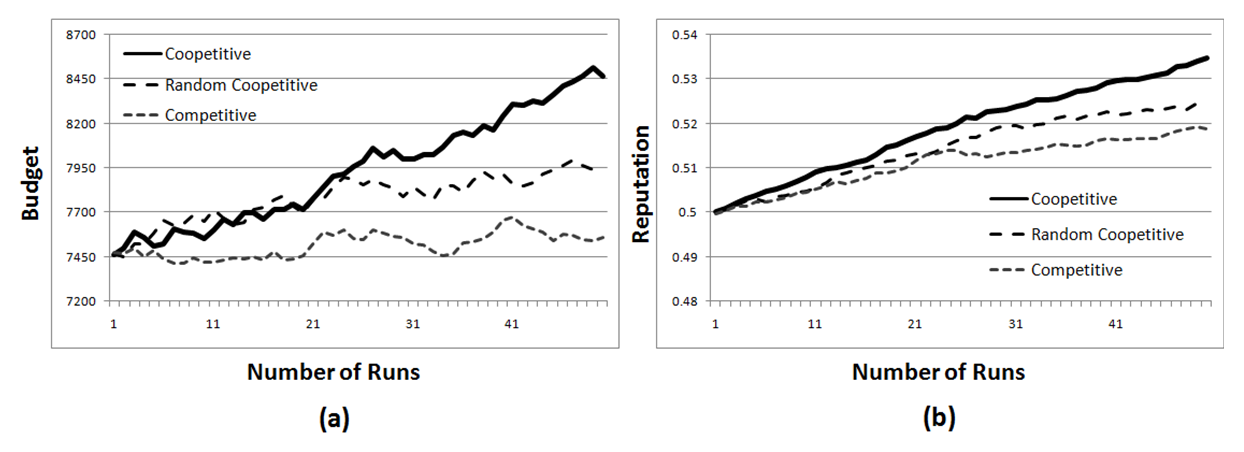
\includegraphics[scale=0.6]{graph1Final+.eps}
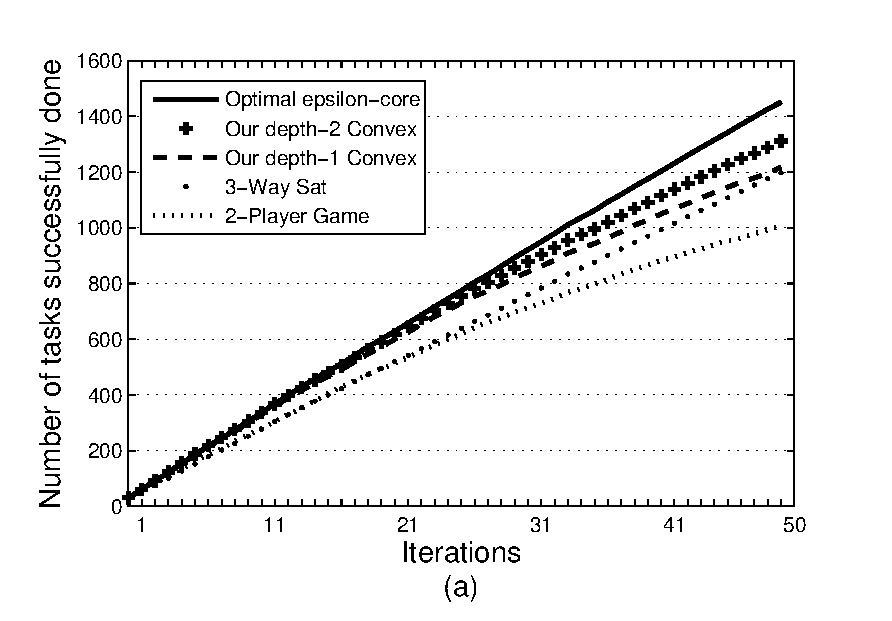
\includegraphics[width=3.5in]{Figures/task_done_opt.eps}
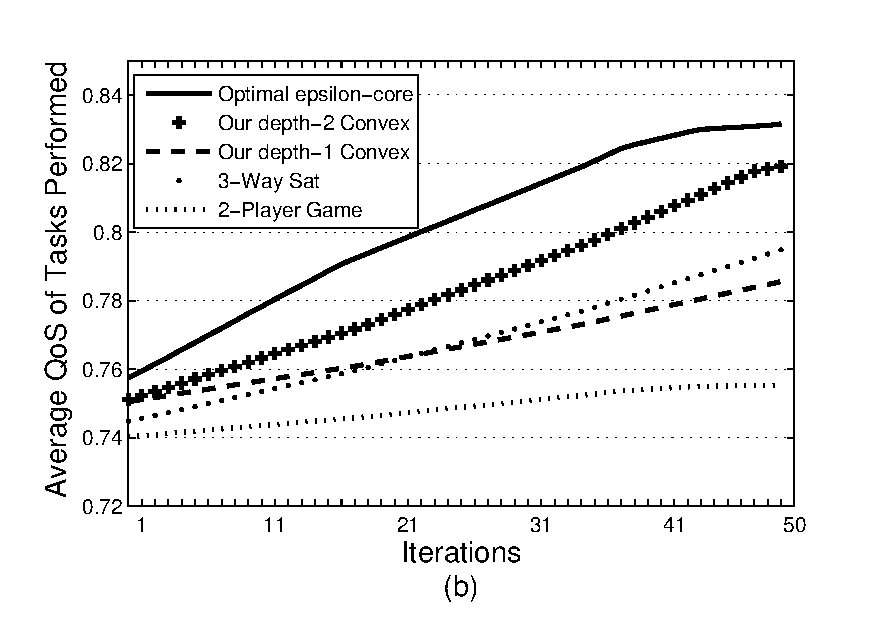
\includegraphics[width=3.5in]{Figures/task_qos_opt.eps}
\caption{Part (a): Cumulative number of requests successfully
done. Part (b): Average QoS of requests performed.}
\label{performanceall}
\end{figure}

Figure \ref{performanceall} depicts the results of optimal
\emph{$\epsilon$-core}, \emph{Depth-1 Convex-Checker},
\emph{Depth-2 Convex-Checker}, \emph{3-Way Satisfaction}
\cite{DBLP:conf/IEEEscc/LimTMB12}, and \emph{2 Player
Non-Cooperative} \cite{DBLP:conf/IEEEscc/KhosravifarABT11} methods
in \emph{one grand community with many web services} scenario.

For the \emph{optimal core} method we have used the well known \emph{$\epsilon$-core} method as the
taxtation method to relax the core condition to help communities, attract web services.
We have assigned $\epsilon$ to 15\% of total community worth, $\epsilon = 0.15 \times v(C)$, which allows
subsets of the coalition to gain maximum 15\% of $v(C)$. In the
\emph{optimal $\epsilon$-core} method, we capped the coalition
size to 25 web services, since the method is computationally
intractable as number of web services increase and anything more than that would make it
impractical to run in our simulations. In the other methods, there
were no cap on size of the community and we had communities of
size 60 web services at some points. In this scenario our community receives 30 tasks on average per iteration, from users. The community, after the task distribution process on each iteration, will reevaluate QoS metrics of its members and can check for new membership requests. Web services may join or leave the community between iterations. The results show that our
\emph{depth-2 convex checker} method is performing better compared
to the other methods and its performance is close to optimal
\emph{$\epsilon$-core} method. Our \emph{depth-1 convex checker}
and the \emph{3-Way Satisfaction} method, are also performing well.

\begin{figure}[!t]
\centering
%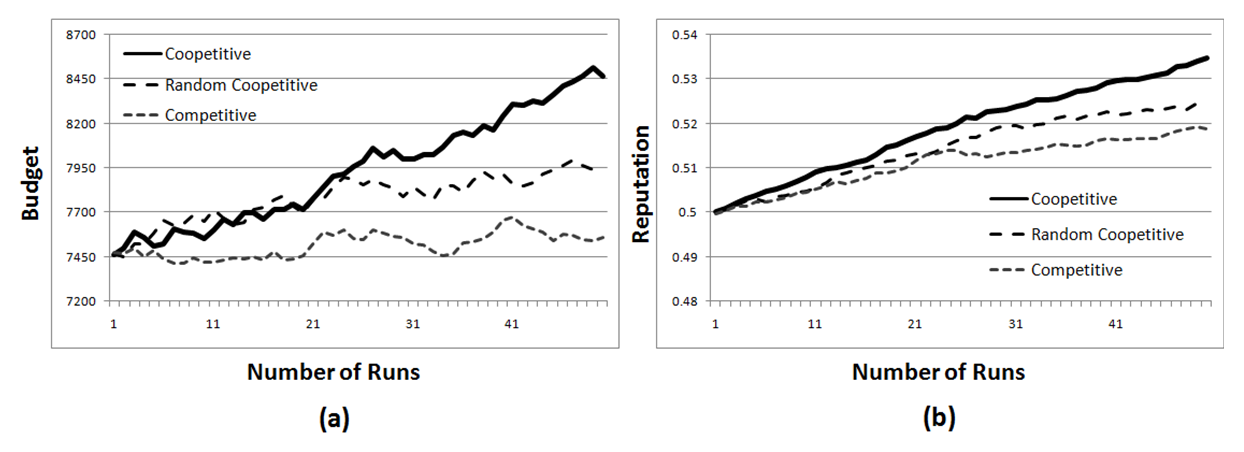
\includegraphics[scale=0.6]{graph1Final+.eps}
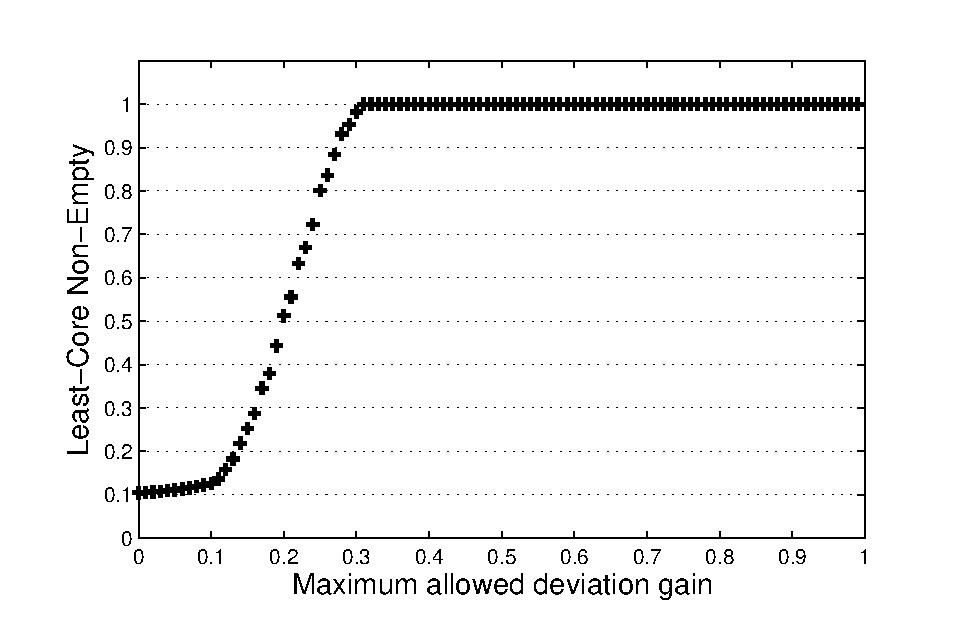
\includegraphics[width=3.5in]{Figures/least_core.eps}
\caption{Analysis of \emph{$\epsilon$-core} set non-emptiness, for different values of $\epsilon$} \label{f_leastcore}
\end{figure}

As mentioned in Section \ref{s:preliminaries}, the concept of
\emph{core}, assumes no coalition of players can gain anything by
deviating, which is a fairly strong requirement, and that is why
the notion of \emph{$\epsilon$-core} was introduced. Least-Core
$e(G)$ of a game $G$, is the minimum amount of $\epsilon$ so that
the core is not empty. We evaluated the non-emptiness of \emph{$\epsilon$-core} set using the
valuation function and a set of web services. We picked random
number of web services from the dataset and formed around 10,000
random coalitions consisting of 3 to 26 web services. We choose 26
as the maximum number of members in our coalition since it
is computationally very complex for larger coalitions to verify whether
\emph{$\epsilon$-core} set is empty or not. Also instead of considering $\epsilon$ amount of constant deviation in \emph{$\epsilon$-core} definition (Equation \ref{eq:core2}), we similarly defined \emph{relative $\epsilon$-core} concept where no coalition would benefit more than \emph{$\epsilon$ $\times$ v(C)} by deviating. We set $\epsilon$ between 0 and 1 and verify the \emph{relative $\epsilon$-core} set non-emptiness. The results in Figure
\ref{f_leastcore} illustrates that almost 10\% of our random web
service coalitions have non-empty \emph{core} solution and
\emph{$\epsilon$-core} solution is \emph{always} non-empty when we
let agents gain only 30\% more of $v(C)$ by deviating.

One of the properties of coalition structure formation algorithms
in our second scenario is that they partition web services with low
throughput rate so that they usually join coalitions with less
request rate. Since the characteristic function $v(C)$ and the
fair Shapely payoff vector is proportional to web services'
contribution, the web services with small contribution will get
paid much less in communities having web services with high
throughput. On the other hand, according to the valuation function
$v(C)$, web services with high throughput will not contribute well
to communities with low amount of user requests (low market
share). The strong web services are likely to deviate from weak
coalitions, joining a stronger one, which makes the initial
coalition unstable.


\begin{figure}[!t]
\centering
%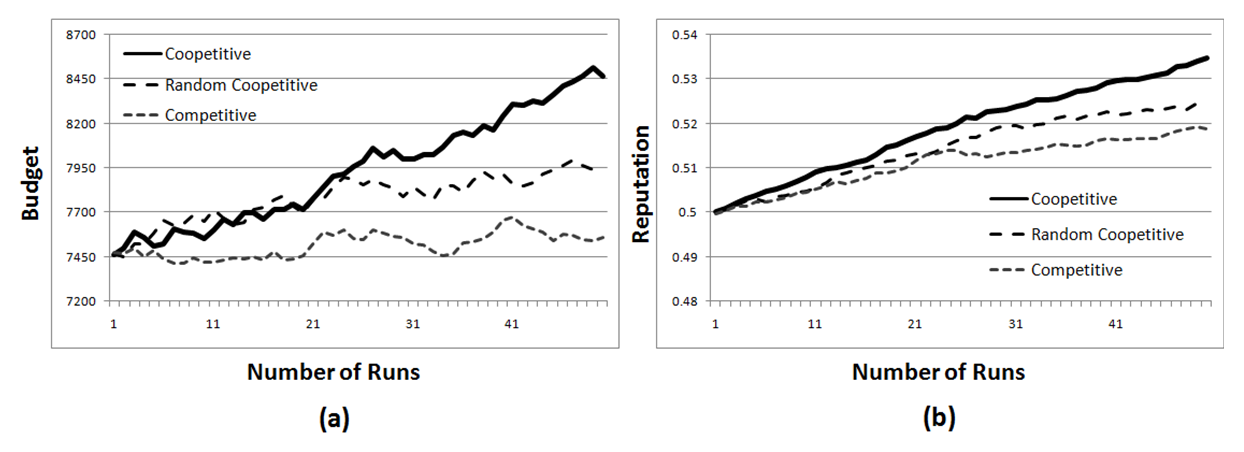
\includegraphics[scale=0.6]{graph1Final+.eps}
\includegraphics[width=3.5in]{Figures/s2_task_done.eps}
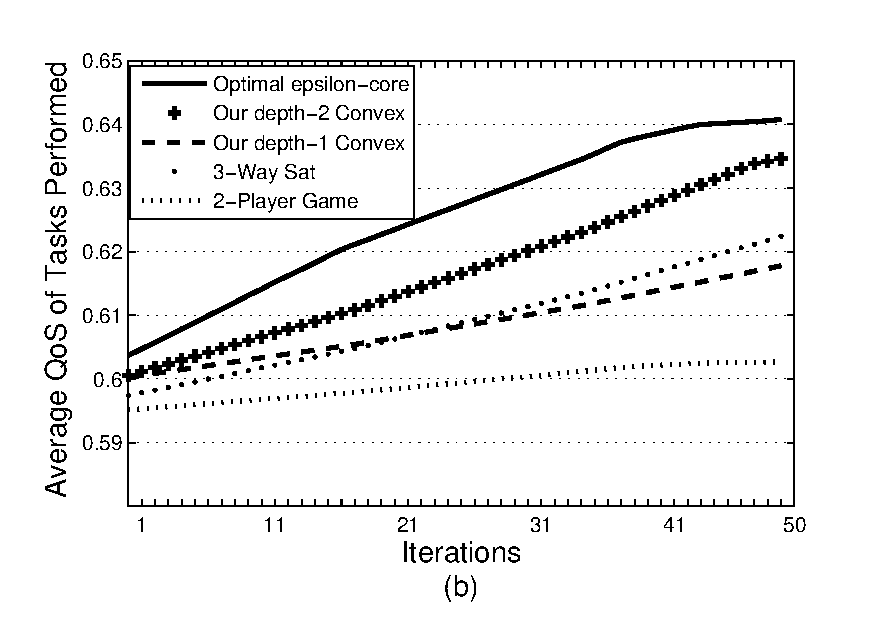
\includegraphics[width=3.5in]{Figures/s2_task_qos.eps}
\caption{Part (a): Cumulative number of tasks succesfully done. Part
(b): Average QoS of tasks performed.} \label{performancemany}
\end{figure}

In Figure \ref{performancemany}, we compare our \emph{Web Services
and many Communities} scenario with a method which ignores QoS
parameters and forms coalitions by allowing web services to join
only if they have enough requests for themselves. In other words,
web services can join a community when the request rate is less
than the throughput of all the member web services. We name this
method \emph{Random Formation} and use it as a benchmark for our
QoS-aware coalition formation process. In this scenario, each user individually generates randomly
between 0 to 10 number of tasks per iteration, then the users target a community and direct their requests to the chosen community. As the results illustrate,
our method forms better coalitions of web services improving
performance and satisfaction for both web services and coalitions.


\begin{figure*}%[!t]
\centering
%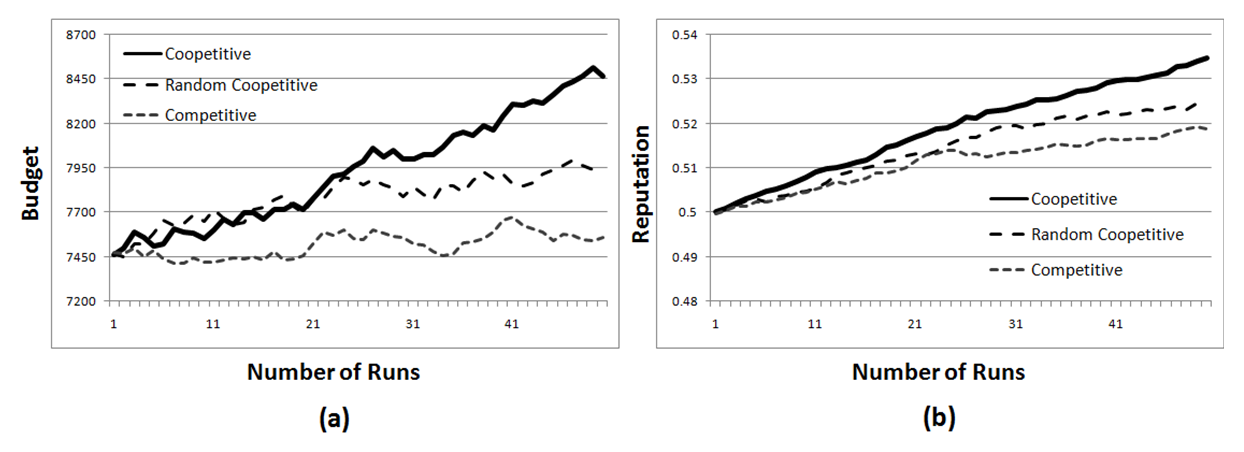
\includegraphics[scale=0.6]{graph1Final+.eps}
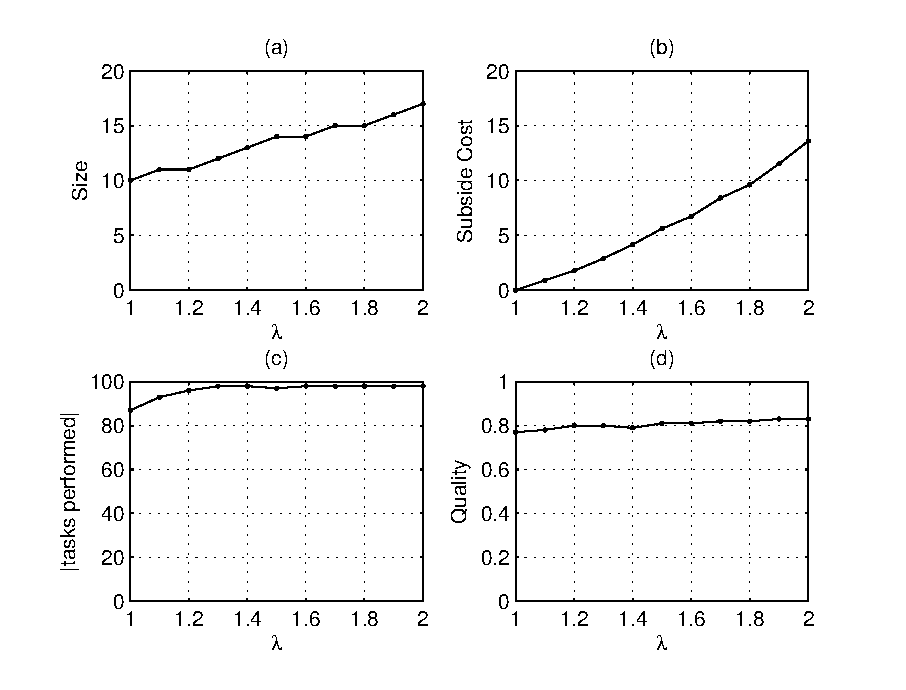
\includegraphics[width=4in]{Figures/taxtation.eps}
\caption{Analysis of community subsiding coefficient $\lambda$ on
average community size (a), cost (b), number of tasks performed
(c), and average quality of service of tasks performed (d).}
\label{f_taxtation}
\end{figure*}

As mentioned in Section \ref{s:tax}, a solution to help the
community stabilize is to subside the community by a relative
coefficient ($\lambda$) so the value of $\lambda v(C)$ is divided
among the community members. We have analyzed the effect of
subsiding and the cost it incurs to our web service communities.
Figure \ref{f_taxtation} shows the results. In this experiment, we
have set a community with input task rate $R_C$ of 100 and having
web services throughput rate $Th_{ws}$ values from a normal
distribution with average 10 tasks per iteration and standard
deviation 2. Part (a) shows the community size increases in a
linear fashion as ($\lambda$) increases. However, the cost (Part
(b)) is having a slight exponential growth rate since, not only
($\lambda$) increases, but also the size of the community is
increasing slowly. Therefore, subsiding can be costly for larger
number of $\lambda$ values. Part (c) depicts the number of tasks
done by the community per iteration. It is obvious that with
$\lambda$ value of 1.3, which is 30\% of the community valuation,
the number of tasks done almost reaches the input task rate cap of
100 tasks per iteration. The average quality of tasks also has a
slight increase since the community will be able to afford better
and more web services to join the community (Part (d)). These
results show the effectiveness of our subsiding method and its
impact on the QoS. In fact, using more than 30\% of the community
valuation as subsidy is not very effective and is costly to
perform.

\begin{figure*}%[!t]In the previous experiment, we considered the scenario where all
web services are stable, will not leave the group, and will
fulfill their promised QoS for a good period of time. However, in
real world scenarios of web services, this is not always the case.
This is the reason why the community coordinator would be interested in paying
web services in order to keep the group reliable from the end
user's point of view.
\centerline{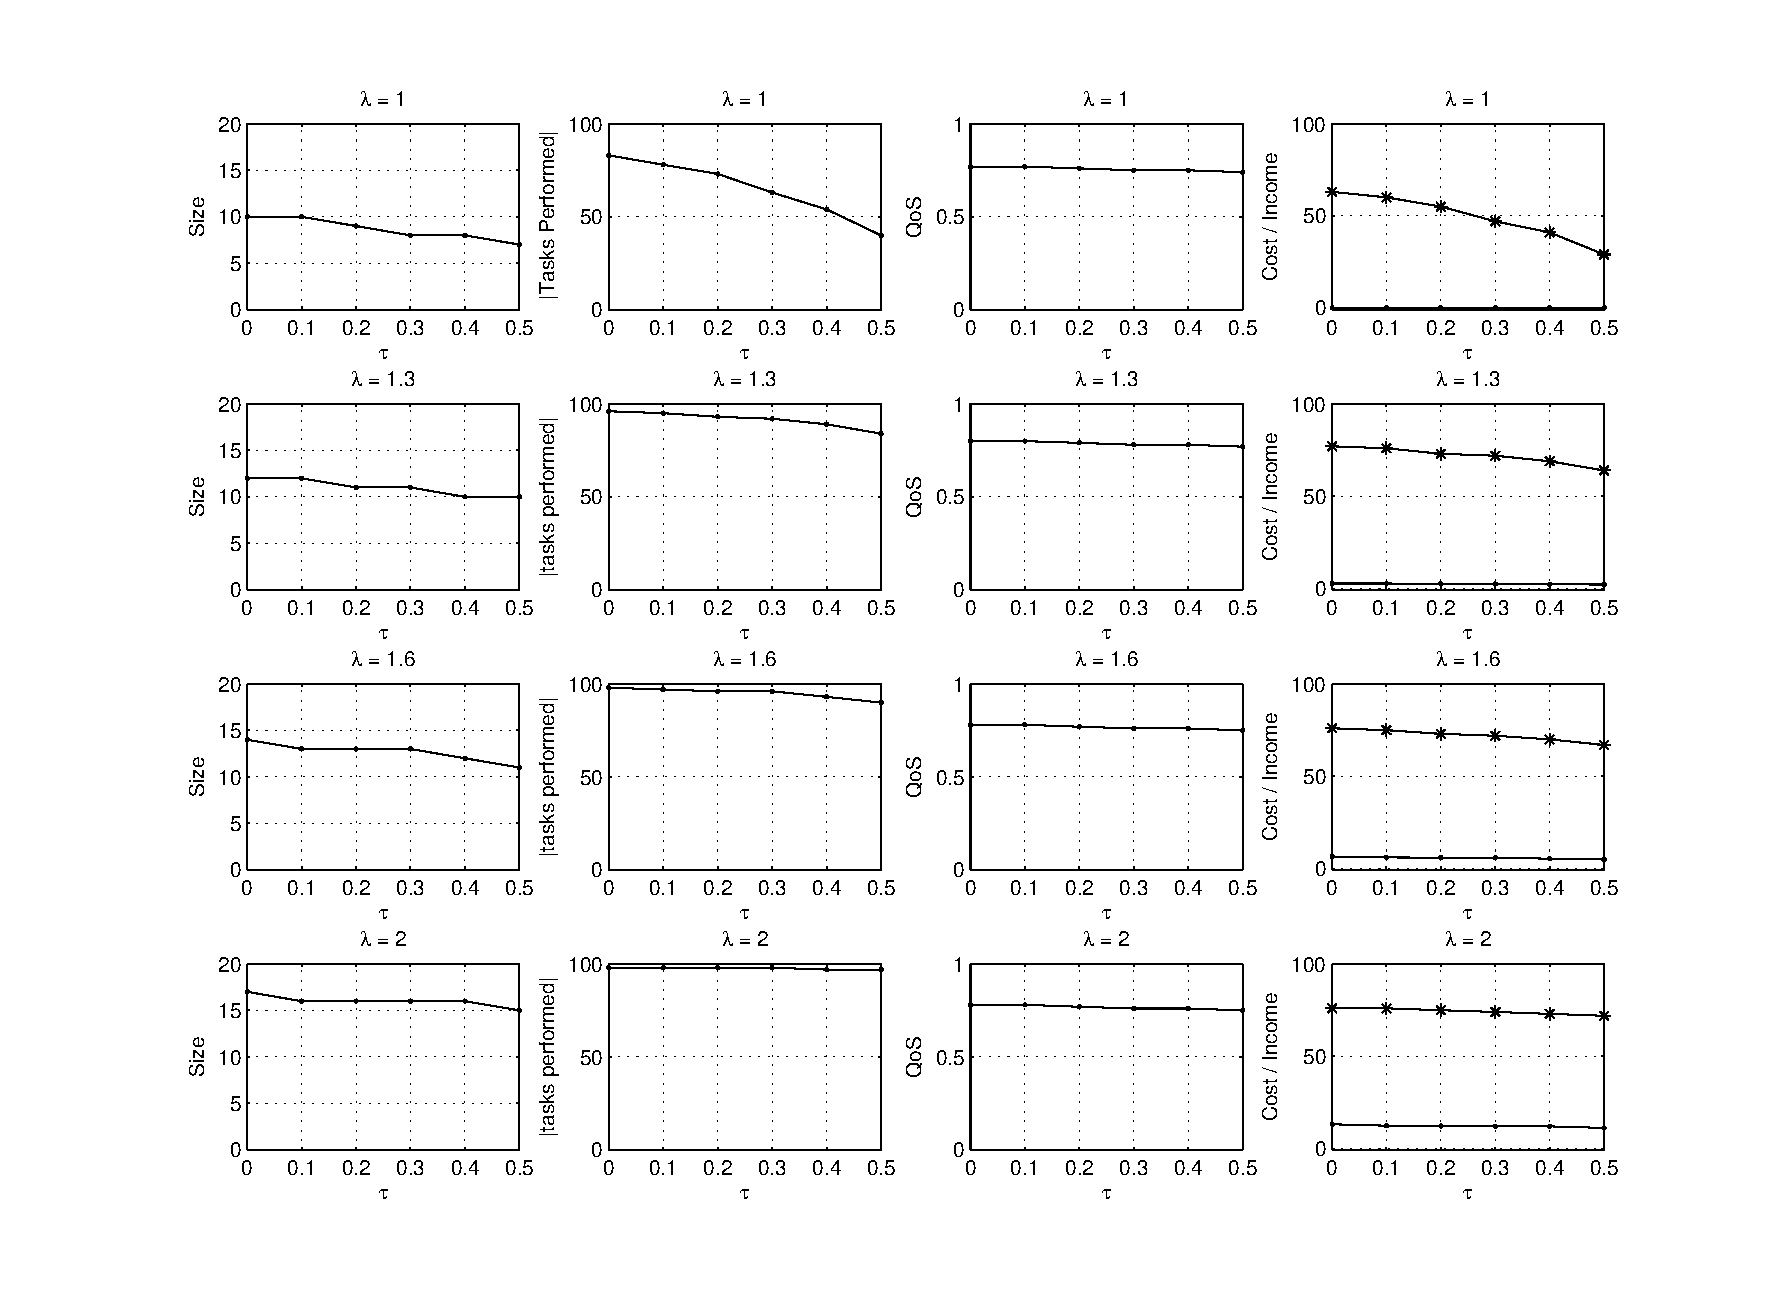
\includegraphics[width=7in]{Figures/tax_dyn.eps}}
\caption{Analysis of community subsiding coefficient $\lambda$
having web service different stability levels of $\tau$ on average
community size, number of tasks performed, average quality of
service, and average cost/income of communities.}
\label{fig_dynamic_taxtation}
\end{figure*}


In our next scenario, we have introduced the
new instability variable $\tau$ ranging from 0 to 1, 0 meaning web
services having no instability issues and will perform as they
claimed until the end of the experiment, and 1 meaning very
unstable web services, which will stop functioning on the first
iteration of the community distributing tasks. Figure
\ref{fig_dynamic_taxtation} illustrates the results of our
experiment having web services with average instability values of
0 to 0.5 and having relative subside value $\lambda$ of 1, 1.3,
1.6, and 2. The \emph{Cost/Income} charts on the right column show
that having subside value of 1.3 incurs the least cost and
increases the community income significantly. Subsiding values of
1.6 and 2 yield high cost to the community and only slightly
increase the community revenue. Moreover, the role of subsiding is
much more obvious when we have unstable web services. In scenarios
where web services are 100\% stable, the subsiding cost will
hardly be compensated by the community revenue.

\begin{figure*}%[!t]
\centering
%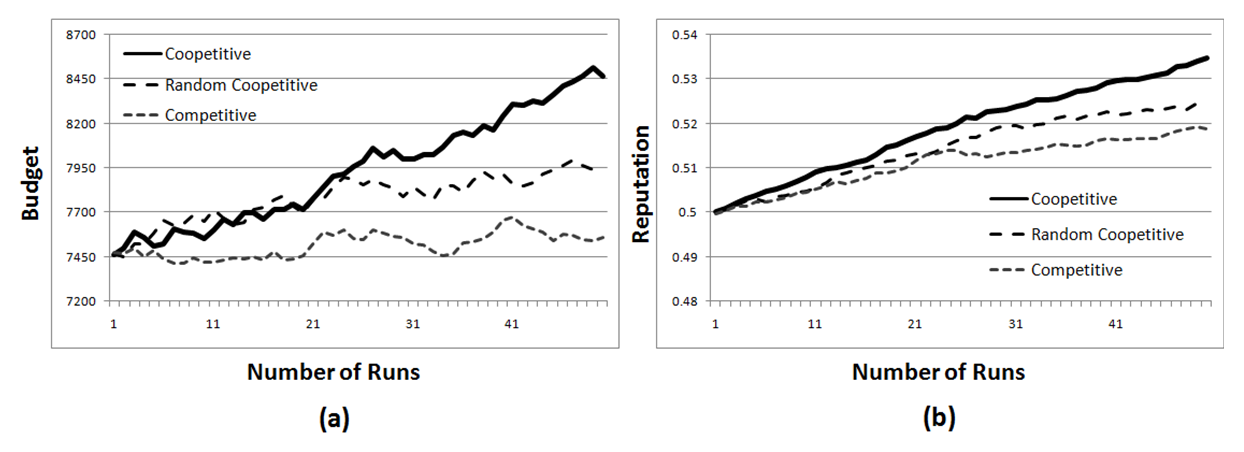
\includegraphics[scale=0.6]{graph1Final+.eps}
\includegraphics[width=3.5in]{Figures/s2_task_done.eps}
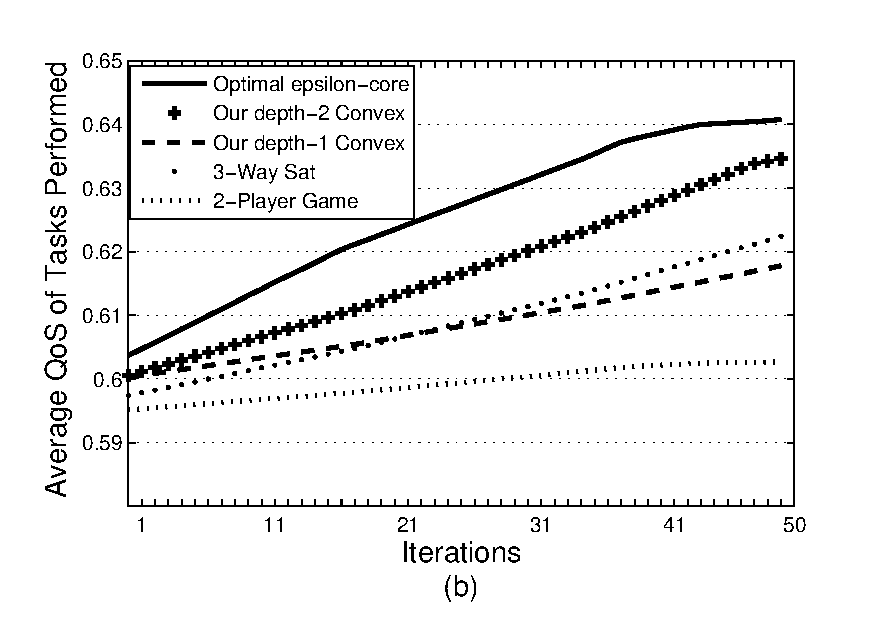
\includegraphics[width=3.5in]{Figures/s2_task_qos.eps}
\caption{Part (a): Cumulative number of tasks successfully done.
Part (b): Average QoS of tasks performed.} \label{performancemany}
\end{figure*}


In Figure \ref{performancemany}, we consider \emph{Web Services
and many Communities} scenario and we compare our dynamic
coalition formation solution with a method which ignores QoS
parameters and forms communities by allowing web services to join
only if they have enough requests for themselves. In other words,
web services can join a community when the request rate is less
than the throughput of all the member web services. We name this
method \emph{Random Formation} and use it as a benchmark for our
QoS-aware community formation process. In this scenario, each user
individually generates randomly between 0 to 10 number of tasks
per iteration, then the users target a community and direct their
requests to the chosen community. As the results illustrate, our
method forms better communities of web services improving
performance and satisfaction for both web services and
communities.

\begin{figure*}%[!t]
\centering
%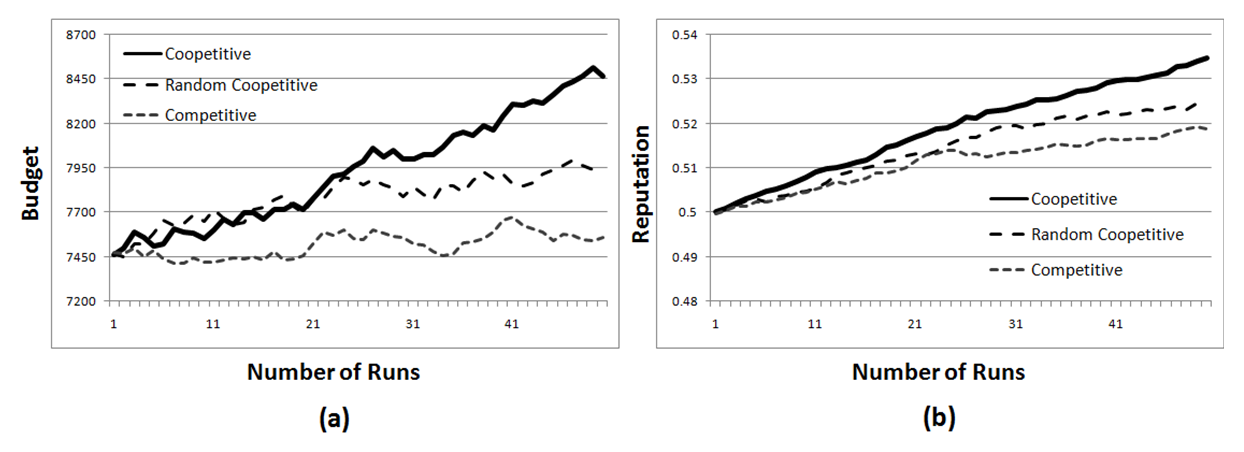
\includegraphics[scale=0.6]{graph1Final+.eps}
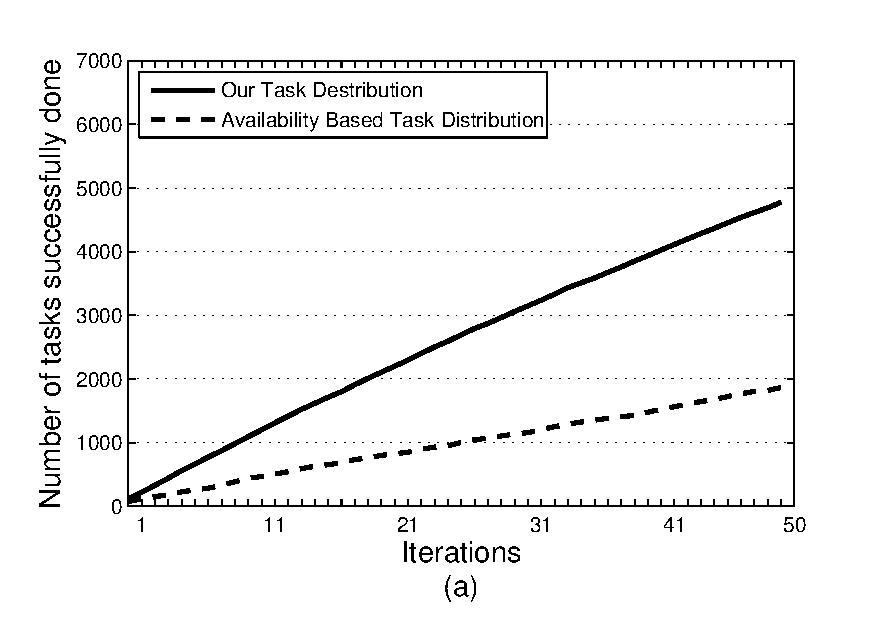
\includegraphics[width=3.5in]{Figures/avg_task_ws_done.eps}
\includegraphics[width=3.5in]{Figures/avg_qos_ws_done.eps}
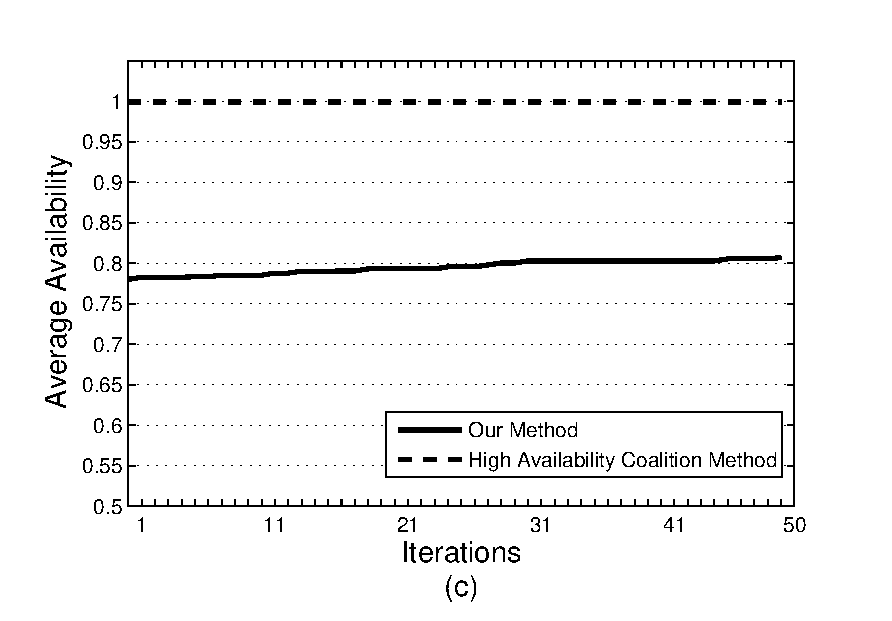
\includegraphics[width=3.5in]{Figures/avg_avail_ws_done.eps}
\caption{A comparison between our community model and the High
Availability Coalition model from \cite{10.1109/TSC.2012.12}. Part
(a): Cumulative number of tasks successfully done. Part (b):
Average QoS of tasks performed. Part (c): Average community
service availability} \label{fig_avail_method}
\end{figure*}

Finally, in our last experiment, we compare our model with the
solution proposed in \cite{10.1109/TSC.2012.12}, which we call
\emph{High Availability Coalition} model. In this method, the
community valuation function focuses on the community availability
as main consideration. The community formation model used in this
method is very different from ours, but we have been very careful
to make the experiment environment as fair and similar to ours as
possible. We limited our maximum community size to 5 in order to
have communities with almost the same size as in
\cite{10.1109/TSC.2012.12}. In the High Availability Coalition
model, the authors have used web services as backups rather than
active collaborative players, and those web services only get a
task when the first web service in an ordered chain fails to
perform that task. %However, with recent advancement in cloud and
%hardware infrastructures, availability is less of an issue for web
%services, and web services are highly available.
Part(a) of Figure \ref{fig_avail_method} shows that with our
method, the number of tasks successfully done is higher with a
rate of three times more than the High Availability Coalition
model thanks to the cooperative behavior of web services and the
task distribution process of our algorithm. This result shows that
using web services as backups, and not as real collaborative
players results in a considerable waste of web services capability
since services have very low chance of getting jobs and its the
primary web service (the first in the coordination chain) which
does most of the work. As shown in Part (b), the average quality
of service of tasks performed using our solution is also higher
since our method considers all quality of service metrics used. Part(c) shows the availability of
communities from the end user's point of view. The High
Availability Coalition model has almost 100\% uptime since web
services are used as backups, so the chance of job failing is
getting reduced significantly as community members increase. In
our method, we have more chance of failure for each web service.
However, with some subsidies and by hiring a few more web
services, the chance of failure of web services in our communities
can be lowered.

%%%%%%%%%%%%%%%%%%%%%%%%%%%%%%%%%%%%%%
\section{Summary}\label{sec:conclusion-cha3}

In this chapter, we proposed a cooperative game theory-based model for the aggregation of web services within communities. The goal of our services is to maximize efficiency by collaborating and forming stable coalitions. Our method considers stability and fairness for all web services within a community and offers an applicable mechanism for membership requests and selection of web services. The ultimate goal is to increase revenue by improving user satisfaction, which comes from the ability to perform more
tasks with high quality. Simulation results show that our, polynomial in complexity, approximation algorithms provide web services and community owners with applicable and near-optimal
decision making mechanisms.

%As future work in this area, we would like to perform more analytical and theoretical analysis on the convexity condition and also minimal $\epsilon$ values in \emph{$\epsilon$-core} solution concepts based on the characteristic function in web service applications. From web service perspective, the work can be extended to consider web service compositions where a group of web services having different set of skills cooperate to perform composite tasks. Also bargaining theory from cooperating game theory concepts can be used to help web services resolve the instability and unfairness issues by side payments.

In this chapter, we assumed our web services and communities have compelte knowledge of all the other web services and their parameters. In next chapter we propose distributed decision making model which can perform in scenarios where information is incomplete.


%%%%%%%%%%%%%%%%%%%%%%%%%%%%%%%%%%%%%%%%%%%%%%%%%%%%%%%%%%%%%%%%%%%%%%%%%%%%%%%
%% Chapter 4: On the Interaction between Probabilistic Knowledge and Probabilistic Commitment.
%%%%%%%%%%%%%%%%%%%%%%%%%%%%%%%%%%%%%%%%%%%%%%%%%%%%%%%%%%%%%%%%%%%%%%%%%%%%%%%
\setcounter{chapter}{3}

\chapter{Distributed Decision Making for Dynamic Formation of Web Services Communities}\label{cha:PCTLKC}


\section{Introduction}

Over the past years, online services have become an important part of many scalable business applications. The increasing reliance on online service providers has significantly influenced the way web services are engineered. Given the dynamic and unpredictable nature of the Internet, delivering high quality services is still a critical and challenging issue. One practical solution towards delivering such quality services is utilizing intelligent decision making agents. These agents aim at maximizing their gain by exploring the best ways to provide services that satisfy end users \cite{Zeng:2003:QDW:775152.775211, 10.1109/ARES.2008.7, Demirkan2013412, journals/tsc/ZhengZYB13, Josang:2007:STR:1225318.1225716}. However, agent-based web services are functionally limited in the sense that they cannot handle a large number of requests at the same time without compromising the quality of service provided. Recent developments have attempted to shift web services from simple models, consisting of individual components, to models made up of autonomous and group-based components that share common goals. In group-based models, interaction, composition, and cooperation are the key challenges that directly impact the group's overall performance in achieving common goals \cite{ICWS2011-1, SCC2011-1, journals/mags/BaldoniBM10, journals/jcss/CasadoYT13}. To that end, we see the emergence of web service \emph{communities}, which consist of grouping services with similar functionalities but distinct nonfunctional properties \cite{Zeng:2003:QDW:775152.775211, 10.1109/ARES.2008.7, Paik:2005:TSS:2229263.2230038, Medjahed05adynamic}. A community of web services runs continuous performance assessment functions that regulate web services' interactions and manage their composition and cooperation.

Web Service communities have the advantages of facilitating web service discovery and providing better quality of service compared to individual services. Communities act as abstract web services, communicating with external entities via the same standard protocols that a normal web service employs. The difference is that communities regulate the service process via sophisticated internal communication protocols, thereby providing services based on the combined efforts of a number of web services. The downside to communities is the complexity of management involved in finding and inviting adequate individual services and managing the overall quality of the combined work of several services.
% because although they have similar functionality, they have different attitudes.
When interacting with a community of web services, users send their requests to the coordinator of the community, which plays the role of community representative or access point. The community coordinator is responsible of receiving tasks and delivering services. Moreover, as community representative, it verifies the credentials of new web services before accepting them into the community and kicks services that could harm the value of the community.

\textbf{Challenges and Problem Statement.} In recent work, communities of web services have been proposed in order to facilitate discovery of web services, improve the Quality of Service (QoS), and help individual services find better market share and opportunities \cite{Zeng:2003:QDW:775152.775211, 10.1109/ARES.2008.7, Paik:2005:TSS:2229263.2230038, Medjahed05adynamic}. However,  two important challenges are to be addressed: 1) choice of the best web services during community development from the community perspective; and 2) choice of the best community to join from the web service perspective. The advocated solutions  \cite{10.1109/ARES.2008.7, conf/webist/MaamarLBTS07, journals/soca/XuYLZB11, 10.1109/TSC.2012.12, managing-hela-jalel, DBLP:conf/IEEEscc/KhosravifarABT11, DBLP:conf/IEEEscc/LimTMB12} have attempted to address these challenges. However, those solutions have two main limits:
\begin{enumerate}
	\item The solutions consider the architecture of centralized management for communities where most of the decisions are made by the centralized coordinator. The problem is that in real world scenarios, decisions made by independent service providers are highly distributed.
	\item The solutions either propose complex algorithms \cite{10.1109/TSC.2012.12, DBLP:conf/IEEEscc/LimTMB12, journal-community-formation} to find the optimal strategy to follow, or oversimplify the problem by eliminating important parameters and using approximation techniques to make the algorithms tractable \cite{10.1109/TSC.2012.12}.
\end{enumerate}
These approximation methods sometimes negatively influence the outcome because simplifying the constraints may cause important aspects of the problem to be ignored. For instance, instead of calculating the gain distribution using the adequate, but complex shapely-value method, the authors is \cite{10.1109/TSC.2012.12} propose a simple egalitarian way of distributing gain, which completely ignores the gain generated from collaborative work of sub-communities. Other categories of related work, for instance \cite{10.1109/TSC.2012.12, DBLP:conf/IEEEscc/KhosravifarABT11, DBLP:journals/ijebr/MaamarSTBB09}, restrict the decision process within the community coordinator, so other members of the community are not effectively involved.
%And some other work which do not focus on rationality on web services or communities involved [refrences].
In \cite{journal-community-formation}, we proposed a cooperative game-theory-based model for aggregating web services in communities. A centralized decision maker in communities, based on a complete knowledge of available web service quality metrics and performance, has been used to form optimal and stable communities that maximize individual and group income. However, centrality and complete information are strong assumptions, which are not very compatible with real business scenarios.

\textbf{Contributions.} In this chapter, we introduce DDM, a Distributed Decision Making model for community formation that regulates web service agents’ decision making process in terms of cooperating and deciding which group to join and which service to invite for joining. Unlike existing work on community formation, our decision model is extracted from a data model in the form of information obtained from a large number of web services regarding their single and cooperative utilities as well as environmental parameters such as demand, service quality, etc. The generated decision tree improves agents' understanding of the environment and how to select actions that lead towards maximizing their utilities. The advantage of this approach is that the tree, which is initially created from the past data, reflects a comprehensive vision about agents' attitudes in terms of their action selection based on their past experiences. Moreover, the tree is getting continuously updated based on both new received feedback and the outcome of chosen actions. This continuous update makes the approach adapted to any change in the environment.
%The training model deploys a logistic regression algorithm to build a hypothesis function that can thoroughly address the aforementioned research problems.
The decision model provides web services with enough information which helps those services efficiently decide and predict the outcome of their different possible collaborations. This model works in a distributed manner in which services are self-sufficient in their decision making and do not rely on a centralized decision making process. Our findings show that communities of web services can efficiently find the appropriate web service to invite for cooperation as well as allowing a single web service to find the best communities to join. The proposed model can be seen as a recommneder system that suggests beneficial actions for both communities and single services. Communities can consider the decision model and analyze the characteristics of different individual web services and make prudent decisions when inviting a web service to join or accepting a join inquiry initiated from a web service. In general, DDM equips web services with efficient methods for foreseeing how their choices will impact both their short-term and long-term goals; therefore, opting for the best decision available.

To effectively generate the decision model for web services, we used a real dataset to extract web services' individual characteristics and used them to measure outcomes when these services cooperate with one another. The dataset has been extracted from real-world QoS evaluation results from 142 users on 4,532 Web services during 64 different time slots. Combining the available data based on each web service point of view on different time slots, we acquired 5 different unique features for those 4,532 web services. By engineering and extracting these features, we gathered functional and cooperative features for both individual web services and communities in different time slots. We were able to investigate the path a web service might take to achieve the best utility out of effective interactions with others. All the paths and outcomes are labeled to be utilized in the training model. Using cross validation sets, web services are able to compute the optimal hypothesis function (using logistic regression) that can be used to predict outcomes of cooperative work with other individual web services or communities. Our findings show that web services equipped with DDM have by far better outcomes than the ones that either do not cooperate or randomly find communities to join.

\section{Preliminaries and Challenging Issues}\label{s4:preliminaries}
%In this section, we first present the architecture of DDM. We explore the characteristics of intelligent service agents and the features we extract for training. To do this, we first discuss some preliminaries.
In this section, we discuss the preliminary concepts of communities of web services and introduce the challenges behind community formation.

\subsection{Web Services}\label{s:ws}

In the recent years, online services have become a standard part of daily life around the globe. Many modern applications rely on web services from different providers. For instance, many mobile and tablet applications that have limited storage and processing power are merely aggregating information from different online services. Examples are vast, including weather forecasting, ticket selling, shopping apps, local maps and location services.

The World Wide Web Consortium (W3C) defines web services as ``software systems designed to support interoperable machine-to-machine interaction over a network. It has an interface described in a machine-processable format (specifically WSDL). Other systems interact with the web service in a manner prescribed by its description using SOAP messages, typically conveyed using HTTP with XML serialization in conjunction with other Web-related standards''. When developers declare a new web service, it will be
discovered based on its description, which fully discloses its functionalities. Developers also have to declare a public interface and a readable documentation to help other developers when integrating different services \cite{w3cwsdl}. Nowadays, web API, standards that do not require XML-based web service protocols like SOAP and WSDL are also emerging. They are called RESTful (representational state transfer) services, which are moving towards simpler communication protocols.
%They are not restricted
%to XML formats, recently JSON, a human readable and simpler format
%is becoming popular among online service providers.

We are not going to delve into the engineering details of online web service implementation and its protocols in this thesis. We are interested in web services from a business model perspective. Service providers usually charge end users for services they provide. For example, Google has listed pricing and plans for a wide range of services they provide on their web service console page\footnote{$https://code.google.com/apis/console$}.

As in other proposals \cite{journals/mags/BaldoniBM10,10.1109/TSC.2012.12,DBLP:conf/IEEEscc/KhosravifarABT11}, in this paper, we abstract web services as rational agents\footnote{The term rational is used here in the sense that web services are utility maximizers.} that provide services to end users. They aim to maximize their individual income  by receiving enough requests from end users. In order to increase their revenues, web services seek for more tasks if they have the capacity and throughput to do so. Web services can join communities to enhance efficiency by collaborating with others, to have access to broad market share, and for the opportunity to receive a bigger task pool from end users.
Furthermore, the high reliance on web services has resulted in increased quality expectations from end users. Communities of web services can provide higher availability, performance, reliability, and recovery for end users.

\subsection{Web Service Communities}\label{s:wsc}

The community of web services is essentially a virtual group of web services having similar functionalities \cite{DBLP:journals/ijebr/MaamarSTBB09}. Communities aggregate web services and communicate with other entities such as UDDI registries and users, using identical protocols to those used by single web services. Web services join communities to increase utility by having a larger market share and task pool. The community coordinator is responsible for securing the community, managing membership requests from web services and distributing user tasks among the community members. The coordinator tries to attract quality web services to join and keep the community as stable and productive as possible to gain better reputation and user satisfaction, which increases the community's market share. How web services reside within communities and how communities of web services are engineered is described comprehensively in \cite{DBLP:journals/ijebr/MaamarSTBB09}.

\subsection{The Join Challenge}\label{s:tjc}
It has been showed in \cite{10.1109/ARES.2008.7,10.1109/TSC.2012.12,journal-community-formation} that web services can increase their overall utility by collaborating with other web services within communities. This collaboration provides them with better ways of sharing resources and having higher reputation, greater market share and wider visibility. Web services and communities come with different quality metrics, and the long-term outcome depends on these metrics.

The goal of all parties involved in the community is to maximize their long-term outcome while they are operating as part of the community. Web services need to be equipped with a selection strategy to choose from the different possible collaboration groups they can form as well as an estimation method for evaluating the long-term gain of joining different possible communities. Web services need to experiment with different possible collaborative groups in order to estimate their gain over time. However, with a high number of possible communities, it is not possible to test collaboration with random web services. Even if a linear approximate function for estimating utility based on community web services' parameters is adopted, the exponential \footnote{Bell number: $http://en.wikipedia.org/wiki/Bell\_number$} growth rate of the possible number of partitions of web services into communities would make any brute-force type algorithm for the best community selection strategy intractable and impractical in real-world application settings.

\subsection{Join Consequences}\label{s:jc}
It is worth mentioning that a \emph{join} event takes place as a result of interaction between two parties that are looking to expand their collaborations. All actions are chosen in an attempt to enhance the overall outcome. However, the selected action may result in decreasing the overall utility in the long run.
% long term.
This is the case when a single web service joins a community, but the complex process of task allocation eliminates the visibility of that service, which stays idle within the community. This makes the join action of that service a bad decision. The same event might be beneficial for the community, as it hosts a new web service that can engage in performing a new coming task. But overall, in this particular case, if the new web service stays idle for a long period of time, neither side will benefit from collaborating with the other and the join event will result in negative consequences for at least one side's utility.

The more common scenario is when both parties benefit from the joining of a web service to a community. This joining action is then rational as both the web service and community enhance their utilities. However, the community may not be the best choice for the web service. In other words, the web service could have joined a better community if it had enough and accurate knowledge about the surrounding environment. Since the community does enhance its utility, the web service could stay with that community, which results in a non-optimal increase in web service's utility. In the following section, the proposed model provides solutions that effectively address the aforementioned challenges.

\section{The Model Components}\label{s:themodelcomponents}

In this section, we discuss the parameters that we use in the rest of the chapter. Then, we present the task distribution and revenue model of our distributed web services communities.

\subsection{Internal Features}\label{s:if}

With a group of web services having identical or similar functionalities, QoS metrics provide nonfunctional characteristics for optimal candidate selection. Web services quality metrics have been studied and analyzed in various proposals, for instance in in \cite{Ardagna:2007:ASC:1263152.1263531,Menasce:2002:QIW:613357.613758,10.1109/ISSRE.2011.17}. In this chapter, we adopt the most representative QoS properties of those services that highly influence their utility.
%We refer to a typical web service as ws_{i}.

Let $C = \{ws_1,ws_2,..., ws_n\}$ be a community with $n$ web services. We define the following features for the group of web services based on their functional parameters:

\begin{itemize}

  \item \emph{Throughput} is the rate at which a service can process requests. QoS measures can include the maximum throughput or a function that describes how throughput varies with load intensity. Throughput is a positive real number. For a given community $C$, the expected throughput value $(Th_{C})$ can be estimated as the summation of throughput of all the service members $Th_{w}~ (w \in C)$:
	
	\begin{equation}
		 Th_{C} = \sum_{w \in C}{(Th_{w})}
	\end{equation}
	
	\item \emph{Availability} is the percentage of time that a service is operating. It is computed as
the probability that the service operation is accessible. Availability of a web service $A_w$ is a real number in the range $[0, 1]$. For a community $C$, the expected availability $(A_{C})$ considering the members operate in parallel (independently from each other) can be estimated as:
	
	\begin{equation}
		A_{C} = 1-\prod_{w \in C}{(1-A_{w})}
	\end{equation}
	
	\item \emph{Execution Time} is the time a service takes to respond to various types of requests.
	%is the expected delay between the time instant when a request is sent and the time when the result is obtained.
	Execution time is usually measured in milliseconds and can be affected by load intensity, which can be measured in terms of arrival rates (such as requests per second) or number of concurrent requests. This internal feature is a positive integer. For a typical community $C$, the expected execution time $Et_{C}$ can be estimated as the execution time of the bottleneck service which is the service with the slowest execution time $Et_{w}$:
	
	\begin{equation}
		Et_{C} = max_{w \in C}{(Et_{w})}
	\end{equation}
	
	%\item \emph{Data Quality} The ability of a data collection to meet user requirements , defined as the proximity of a value v returned by web service to a value considered as correct. The measure of data quality is considered here as a real number in the range [0, 1], where 1 represents the most desirable score.
\end{itemize}


	We normalize the range of these features so that each feature contributes proportionally to the final utility outcome value. We adopt the \emph{standardization} method consisting of subtracting the \emph{mean} from each feature, then dividing the subtraction result by the \emph{standard deviation}.

%$HI = \overline{HI}$

\subsection{External Features}\label{s:ef}

The quantitative values of quality metrics need some benchmark values to represent their goodness. In fact, without some benchmark values, it would be difficult for web services to identify their performance quality at any specific value of these metrics. Therefore, we introduce two external features for assessing web services' estimate with regard to their standing among other web services.

\begin{itemize}
  \item \emph{External Parameter 1} ($Exp1_i$ where $i$ is a community or a web service) is an estimate of how close the community's or the web service's \emph{execution time} is to the best execution time in the whole system. It is the difference between a community's or a web service's \emph{execution time} metric and the minimum value of execution time of all the other communities or web services. The smaller the value the better the external feature compared to other peers. In other words, small value of $Exp1_i$ means $i$ is among the best communities or services in the system.
	\begin{equation}\label{exp_1:f}
		Exp1_i = Et_{i} - Et_{min}
	\end{equation}
	\item \emph{External Parameter 2} ($Exp2_i$ where $i$ is a community or a web service)  is a comparison of the community's or the web service's rate of performing tasks to the best rate in the system. It is the difference between a community's or a web service's \emph{throughput} metric and the maximum value of throughput in the system. As for $Exp1_i$, the smaller the value the better the external feature.
	\begin{equation}\label{exp_2Lf}
		Exp2_i = Th_{max} - Th_{i}
	\end{equation}
\end{itemize}

\subsection{Task Distribution}

Communities of web services usually employ an implementation of Contract-Net protocol for task distribution, in which services bid on incoming tasks, and receive some of the tasks for which they bid \cite{DBLP:journals/ijebr/MaamarSTBB09,DBLP:conf/aina/ElnaffarMYBT08}. In our model, our community members would try to distribute tasks based on their capabilities and the QoS parameters provided by the web services. We use a slightly modified \emph{weighted fair queuing} method to distribute tasks among community members. The goal is to allocate incoming tasks to web services with a rate matching the throughput value of $Th_{w}$ for each web service $w$. In the \emph{weighted fair queuing} method, the input flow is multiplexed along different paths. However, in our model, if the rate of incoming tasks is less than the community's total throughput $(Th_{C})$, which is the summation of throughput values of the web services in the community, some of the input tasks will be queued and served with a delay.
%Thus, the amount of tasks performed by the community is $\sum_{ws}{Th_{ws}}$ when $\sum_{ws}{Th_{ws}} \leq R_{C}$.
When the incoming task rate is less than the throughput of the community, the \emph{weighted fair queuing} algorithm assigns a weighted task rate of $Itr \times \frac{Th_{w}}{\sum_{w}{Th_{w}}}$ for each web service $w$ within the community, where $Itr$ is the input task rate.

While distributing tasks, the community can verify the performance, throughput and quality of service of tasks being performed by web services. The community can assess if those web services are capable of performing the number of tasks they advertised. If for any reason, there is a decline in the quality metric or throughput, the community can consider the new values as a benchmark for future performance calculations, and penalize the suspicious web services. This way, players will have incentive to truthfully disclose their actual capabilities in order to maximize profit from the community and to avoid being penalized. In addition, the system should be dynamic enough to detect and react to web services' quality metrics variation, as over time, web service metrics may degrade or improve, changes to which the community should adjust.
% Therefore its easy for the system to encourage players to be in some sense incentive compatible in the way that they would profit best by truthfully revealing their capabilities. Also it is important to be dynamic enough to consider web services which may have their quality metrics degraded or even improved over time for any reason and be able to adjust the community with new parameters.

\subsection{Community Revenue}

Communities and web services earn revenue by performing tasks. The total gain is a function of the quality and rate of performing tasks. The utility of a collaborative group of services $U_{C}$ (i.e., the revenue of the community) is a function of internal and external parameters:

\begin{equation}\label{u_c_general}
U_{C} = f(A_{C}, Et_{C}, Exp1_{C}, Exp2_{C}, Th_{C})
\end{equation}
%
where $f$ is increasing in $A_{C}$ and $Th_{C}$ and decreasing in $Et_{C}, Exp1_{C}$ and $Exp2_{C}$. An example of this function is given in Equation \ref{u_c_normal}:

\begin{equation}\label{u_c_normal}
U_{C} = \big((\alpha \times (A_{C} - Et_{C}) - \beta \times (exp1_{C} + exp2_{C})\big) \times Th_{C}
\end{equation}

The $\alpha$ and $\beta$ parameters are internal and external weight coefficients. Small values for execution time and external parameters ensure better performance, which justifies their negative coefficients. The result is then multiplied by the throughput value $Th_{C}$, since communities are performing tasks with $Th_{C}$ rate.

\begin{theorem}
The function given in Equation \ref{u_c_normal} satisfies the properties of $f$.
\end{theorem}

The proof of this theorem is straightforward by simply calculating the partial derivative $\partial f$ with respect to the different variables.


The estimation of the utility can be improved, especially in cases where the input task rate is high and services are experiencing high task loads. The \emph{weighted fair queuing} method of task distribution would distribute tasks based on the individual throughput $(Th_{w})$ value of services within community. In fact, services having higher throughput affect strongly the overall utility of the community because they would take on proportionality more tasks. The improved utility is given as a function of individual internal and external parameters:


\begin{equation}\label{improved_u_c_general}
U_{C} = g_{w\in C}(A_{w}, Et_{w}, Exp1_{w}, Exp2_{w}, Th_{w})
\end{equation}
%
where $g_{w\in C}$ is increasing in $A_{w}$ and $Th_{w}$ and decreasing in $Et_{w}, Exp1_{w}$ and $Exp2_{w}$. An example of this function is given in Equation \ref{u_c_load}:


\begin{equation}\label{u_c_load}
\begin{split}
U_{C} = \sum_{w \in C}&\bigg(\big(\alpha \times (A_{w} - Et_{w}) \\
        & - \beta \times (Exp1_{w} + Exp2_{w})\big) \times Th_{w}\bigg)
\end{split}
\end{equation}

The following theorem holds:

\begin{theorem}
The function given in Equation \ref{u_c_load} satisfies the properties of $g_{w\in C}$.
\end{theorem}


\section{The Decision Making Mechanism}\label{s:model}

In this section, we describe our data extraction process and the methodology used to equip web services and communities with a decision making mechanism. In this methodology, we first present the data extraction and engineering process and then we evaluate the decision making mechanism for web services in community settings. Figure \ref{fig_steps} summarizes the steps performed in DDM from the input data to the generation of decision making profiles for web services and communities. The objective is to use the input data to build a decision tree for each service and community included in the data set, which will be be served as a benchmark for other services and communities in their decision making mechanism. The decision tree is made up by training the real data obtained from operating web services and extracting features related to their performance, either alone or as part of a joint effort with other web services. The ultimate objective is to propose for each web service and community the best joint decision about forming a group that maximizes every one's utility. The DDM's steps are explained in the following sections.

\begin{figure}%[!t]
\centerline{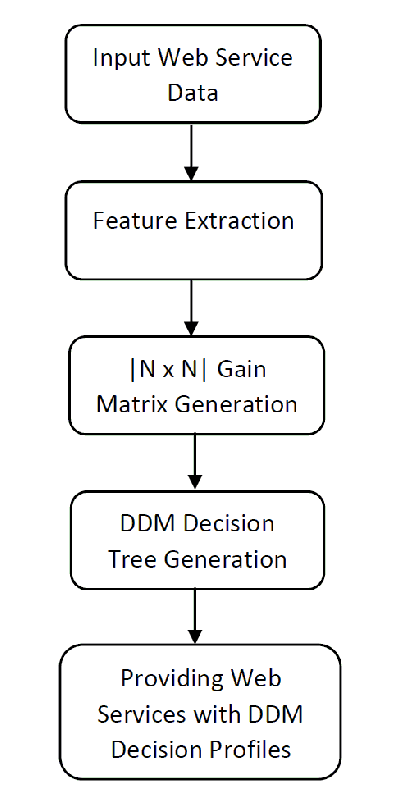
\includegraphics[width=5.25in]{figures/steps.eps}}
\caption{A summary of DDM decision profile generation steps}
\label{fig_steps}
\end{figure}

\subsection{Data Extraction and Solution Engineering}\label{ss:learningdata}

\subsubsection{Input Web Services Data}\label{sss:webservices}

%We used a data set extracted from running web services. In this data set,
Each web service is associated with a number of quality metrics that reflect its non functional parameters. These web services operate in an online environment and are continuously assigned tasks to handle. %To engage in communities, we add the external features that reflect web services' utility as a result of joining other web services to form a community (see Section \ref{s:ef}). %The additional features are %computed based on two assumptions that we adopt for a community to be formed.
We used the web services data set provided in \cite{10.1109/ISSRE.2011.17}. The raw data provides real-world QoS evaluation results from several users on 5,825 web services over 64 different time frames\footnote{http://www.wsdream.net/}. %In this data set, each web service is associated with a number of features that reflect its functionality.
%Our raw data set provides us with 64 different time slots of extracted features for each web service.
Using this data, we built a synthetic data set that contains features of a large number of web services and communities in different time intervals. The goal is to use the data set to train a decision-making model that adopts the trend of joining a community and use the model to predict/find the appropriate community for other web services. %To train our model, we build a decision tree as a benchmark for our decision making mechanism. The decision tree is made up by training the real data obtained from operating web services and extracting features related to their performance, either alone or as part of a joint effort with other web services. The ultimate objective is to propose for each web service and community the best joint decision about forming a group that maximizes every one's utility.

\subsubsection{Feature Extraction}\label{sss:filtereddata}

By processing the data provided for each web service over different time slots, we obtain the three internal quality features introduced in Section \ref{s:if}: \emph{throughput}, \emph{availability} and \emph{execution time} and the two external features discussed in Section \ref{s:ef}.  In fact, web services and communities are represented using feature vectors of these five internal and external features.

%To engage in communities, we add two additional external features that reflect web services estimation of its quality metrics compared to other web services.
%Therefore, we have generated an array of web services with three distinct features.

\begin{figure}%[!t]
\centerline{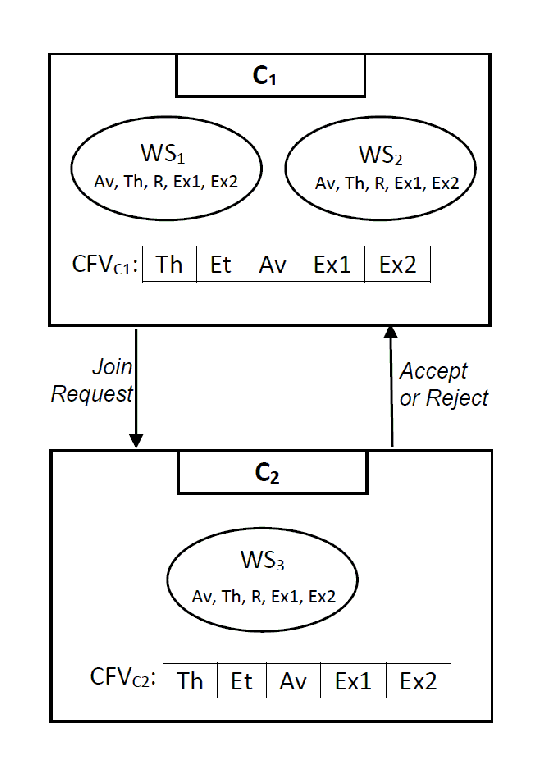
\includegraphics[width=3.15in]{figures/cfvs.eps}}
\caption{Communities with different properties of web services actively looking for other communities to collaborate with}
\label{fig_community}
\end{figure}

%By combining these three internal features to the two external features discussed in Section \ref{s:ef} that reflect the community's estimation of its quality metrics, we generate a set of feature vectors representing the communities of web services for training purposes.


We formulate a \emph{Community Feature Vector (CFV)} as $CFV_{<C>} = [f_1,...f_5]$ having a community of $k$ web services ($C = \{ws_1,...ws_k\}$, $k \geq 1$)\footnote{A web service is considered as a community of one web service.}. The features $f_1$ through $f_5$ represent the \emph{execution time}, \emph{throughput}, \emph{availability} and the \emph{external parameters 1 and 2} respectively. A set of communities, with their feature vectors and utilities evaluated, provides our algorithm with a raw training data set. We call this set of communities the \emph{template vector} $CS$, and the set of feature vectors associated with the \emph{template vector} is referred to as the \emph{community feature vector set (CFVS)}. Figure \ref{fig_community} depicts web services and communities looking to form new groups in order to improve their utility gain.

\subsubsection{Feature Engineering}\label{sss:feng}
Let $CFVS = \{CFV_{<C_1>}, \dots, CFV_{<C_N>}\}$ be the community feature vector set with $N$ communities. Based on the $CFVS$ set, we create an $|N \times N|$ gain matrix $gain^{t}$ for each time slot $t$. Each entry $gain_{n,m}^{t}$ corresponds to a utility gain of community $C_n$ when it joins community $C_m$. This gain is computed as follows: $gain_{n,m}^{t} = U_{C_n \cup C_m}^{t} - U_{C_{n}}^{t}$ where $U_{C_n \cup C_m}^{t}$ and $U_{C_{n}}^{t}$ are the utilities at time $t$ computed using Equation \ref{u_c_load}.  Evaluating the utility gain for all entries of the $gain^t$ matrix is a computationally heavy process when $N$, the size  of the feature vector set, is large. Therefore, this size should be chosen carefully.

\begin{table*}[ht]
\footnotesize
\caption{An example of $gain$ matrix for 3 different communities and their combinations} % title of Table
\centering % used for centering table
{\renewcommand{\arraystretch}{1.2}
\begin{tabular}{c|c c c c c c} % centered columns (4 columns)
\hline\hline %inserts double horizontal lines
 & \textless348\textgreater & \textless1934\textgreater & \textless2117\textgreater & \textless348, 1934\textgreater & \textless1934, 2117\textgreater & \textless348, 1934, 2117\textgreater \\ [0.5ex] % inserts table
%heading
\hline % inserts single horizontal line
\textless348\textgreater & - & 0.282708 & 1.027081 & 0.282708 & 18.027081 & 18.027081 \\
\textless1934\textgreater & -2.637483 & - & 6.969072 & -2.637483 & 5.509583 & 4.387725 \\
\textless2117\textgreater & 5.027081 & 2.969072 & - & 5.509583 & 2.969072 & 5.509583 \\
\textless348, 1934\textgreater & 0.0 & 0.0 & -3.851432 & - & -3.851432 & -3.851432 \\
\textless1934, 2117\textgreater & 2.969072 & 0.0 & 0.0 & 2.969072 & - & 2.969072 \\
\textless348, 1934, 2117\textgreater & 0.0 & 0.0 & 0.0 & 0.0 & 0.0 & - \\ [1ex] % [1ex] adds vertical space
\hline %inserts single line
\end{tabular}
}
\label{table:nonlin} % is used to refer this table in the text
\end{table*}

%Now, we let our set of communities in the $CFVS$ set, within $|T|$ time frame iterations, choose the the best communities to join.
Each community is provided with the corresponding row of data from the $gain^t$ matrix. Basically, $C_i$ is provided with the data in row $i$ of this matrix, which reports all the possible utility values $C_i$ can gain by joining different communities. By ordering the utility gain values of the row, each community is equipped with an ordered set of preferences over other communities it can join. We define $\geq_{i}^t$ as the preference order of community $i$ at time $t$.

Let $C_1 \geq_{i}^t C_2 \geq_{i}^t ~\dots~ C_{i-1} \geq_{i}^t C_{i+1} \geq_{i}^t ~\dots~ C_n$ be an ordered sequence of preferences for community $C_i$ at time $t$. Based on this sequence, we define $K^t(C_i, k)$ as a set of the $k$ most preferred communities of community $i$ at time $t$.
%\subsubsection{feature vector generation}\label{sss:fvg}
\begin{equation}\label{h_t_pref_top}
\begin{split}				
K^t(C_i, 0) = &\emptyset \\
K^t(C_i, k) = &\Big\{C_x | C_x \geq_{i}^t C_y ~\forall C_y \in CS ~\wedge~ C_x \neq C_y ~\wedge~ C_y \notin K^t(C_i, k-1) \Big\}				
\end{split}
\end{equation}
Based on $K^t(C_i, k)$, we define a set of communities $C_j$ for $C_i$ which are the $k$ most preferred communities for $C_i$ and $C_i$ belongs to the $k$ most preferred communities of $C_j$. This basically yields the preference in both sides.
\begin{equation}\label{l_t_top_both}
\begin{split}	
L^t(C_i,k) = \Big\{C_j | C_j \in K^t(C_i, k)~ \wedge~ C_i \in K^t(C_j, k)\Big\}
\end{split}
\end{equation}

Table \ref{table:nonlin} illustrates an example of a $gain$ matrix for 3 different communities and their combinations. Each row shows the gain the community can achieve by collaborating with other 5 communities. In this example, for community $\textless 348 \textgreater$ we have: \\
$K(\textless 348 \textgreater, 1) = \{\textless1934, 2117\textgreater\}$ and \\
$K(\textless 348 \textgreater, 2) = \{\textless1934, 2117\textgreater, \textless1934\textgreater\}$ \\
Since $\textless 348 \textgreater$ is the best preferred community of $\textless 1934, 2117 \textgreater$ and vice versa, therefore $L(\textless 348 \textgreater, 1)$ is not empty and contains the community $\textless1934, 2117\textgreater$.

Using the $gain$ matrix and the mentioned preference ordering relations, we are able to build a decision tree where the list of possible communities to join and their expected utilities are set.
% as well as the joined events that took place in different time slots.
In addition to the best choice, web services have access to other ordered choices and can look for the second best or third best if their first try is rejected by the target community. This aspect is analyzed in more detail in the following section, in which we launch experiments and investigate the effectiveness of the use of a decision tree with different decision layers in joining other communities and enhancing the overall utility.

\subsection{Decision Profile Generation}\label{ss:learningmodel}

Our goal is to create a decision making profile for each community in the
$CFVS$ set. We are creating an environment where the communities can experience the
outcomes of different strategies. The result will be a decision tree of the
feasible and utility-increasing moves over time. The root of the decision tree
represents a community in the $CFVS$ set, and the other nodes represent
the communities resulting from the parent node's action of joining them along with their feature values and
expected utility.


We let communities pick the best communities maximizing their utilities over different time frames. At time $t = 1$, we let each community in the $CFVS$ set choose the best community, which is a single community in the set $\{C_j\} = K^t(C_i, 1)$. If community $C_j$ also ranks $C_i$ to be the highest preferred community to join, meaning the set $L^t(C_i, k=1)$ is not empty, they would join each other. Having set $k = 1$ is a very strict and hardly satisfiable condition. In order to relax the requirement, we increase the value of $k$ by a rate $r$ proportional to time slot $t$: $k = 1 + |r \times t|$. On early steps of the training process, web services and communities are more strict, but as time goes on, we let them choose second and then third best options too. However, increasing $k$  increases the time complexity as well.

When communities $C_i$ and $C_j$ are in each other's top $k$ preference set, the new combined community, i.e., $C_i \cup C_j$ is added to the list of possible communities that can join others at time $t+1$. Moreover, for each community $C_i$ in our initial $CFVS$ set, we maintain a tree with the community $C_i$ as its root. Its children are all the communities that $C_i$ decided to join. As the scenario progresses over time, the merged communities may decide to join other communities. When communities $C_i$ and $C_j$ decide to join each other and create community $C_k$, the new community $C_k$ will be added as a child to both $C_i$ and $C_j$ nodes. At the end of the process, each community is utilized with a tree representing all possible combinations of communities it can join. Algorithm \ref{algo:dectree} illustrates the DDM tree creation procedure as pseudo-code.

\begin{algorithm}
\DontPrintSemicolon
\KwIn{$\langle r, gain^t_{n,n}, CFVS \rangle$ learning rate $r$, $|N \times N \times T|$ gain matrix, community feature vector}
\KwOut{A set of \emph{root} nodes of the decision trees}
$k \gets 1$\;
$nodes[N] \gets$ initialize $N$ tree nodes representing each community in CFVS\;
\For{$t \gets 1$ \textbf{to} $T$} {
	$k \gets 1 + round (r \times t)$\;
  \For{all $C_i \in CFVS$} {
	  \For{all $C_j \in L^t(C_i, k)$} {
      % The "l" before the If makes it so it does not expand to a second line
      \If{$C_i \in L^t(C_j, k)$}{
        $C_k \gets C_i \cup C_j$\;
				add $C_k$ to $CFVS$ set\;
				initiate $node_k$, representing $C_k$\;
				$nodes_i.addChild (node_k)$\;
				$nodes_j.addChild (node_k)$\;
      }
%      \Else{
%        $j \gets j + 1$\;
%      }			
		}
  }
%  $i \gets i + 1$\;
}
\Return{nodes}\;
\caption{{\sc DDM Decision Tree Algorithm}}
\label{algo:dectree}
\end{algorithm}

Having created $|n|$ trees, one per community, our communities are utilized with the different possible paths they can take to maximize their utilities. Using a distance function\footnote{See Section \ref{s:experiments} for an example of this function.}, communities and web services outside the training set can find the community that closely resembles their parameters within the $CFVS$ set. Those new communities can use the trees of the closest communities in the training set to have an estimation of the outcome of all possible joining actions they can take. By so doing, new communities can request to join the best communities which will maximize their gain. Such a request is most likely to be accepted as the decision considers the preferences and utility gain of the other side as well.

As a real scenario example from the used data set, Figure \ref{fig_tree} depicts a snapshot from a decision tree created by the DDM algorithm for a particular singleton community $C_{1273}$. This tree shows the different communities that $C_{1273}$ has experienced with during the training process. Each line shows the web services list within a community, the community's feature vector and the last value on each line is the overall gained  utility of the community.


\begin{figure}%[!t]
\centerline{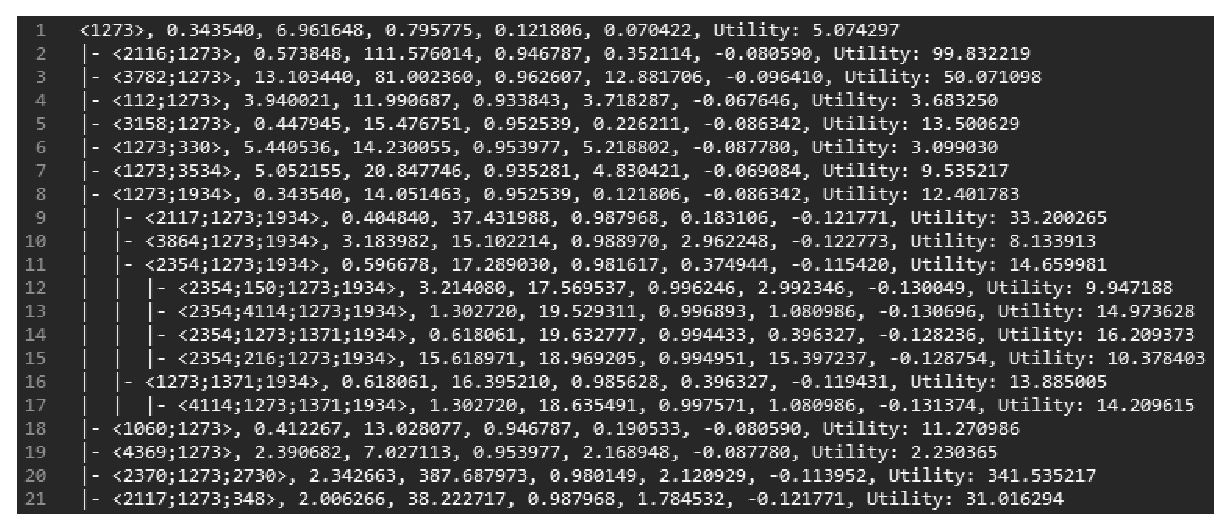
\includegraphics[width=6.25in]{figures/tree1.eps}}
\caption{A partial view of a decision tree created by DDM}
\label{fig_tree}
\end{figure}

\textbf{Complexity.} Here we analyze the computational complexity of the DDM decision tree creation algorithm on each time iteration $t$. Computing top $k$ preferred communities for $C_i$ in $K^t(C_i, k)$ requires $O(n.log(n))$ sort time. The size of $K^t(C_i, k)$ is $k$, and for each of those $k$ communities, we need to check against their $k$ top preferred communities, which needs $O(k^2)$. Line 5 iterates through $n$ communities, Line 6 takes $O(n.log(n))$ to compute and iterates $k$ times, and considering we already have the list sorted, Line 7 can reuse the sorted preferences. Thus, Line 7 takes $O(k)$ time to check if $C_i$ is member of $K^t(C_i, k)$. Multiplying these iterations, the order of complexity of the algorithm with regard to $n$ and $k$ for each time slot is: $O(k^2 \times n^2.log(n))$. Since the whole algorithm runs $T$ times, the overall complexity is $O(T \times k^2 \times n^2.log(n))$.

\section{Experiments}\label{s:experiments}
We implemented DDM in Java\footnote{Source code of implementation and data is available at: $https://github.com/Marooned202/DDM$}. We recall that we have extracted the set of features for 4532 web services in 64 different time slots through a data set provided in \cite{10.1109/ISSRE.2011.17}. By randomly choosing 86 web services out of this data set for each run, and selecting a subset of all possible combinations of sizes 2, 3, and 4 of these 86 web services, we have been able to create 10,000 communities and evaluated the feature vectors and utilities they can have in the 64 time slots. This provides us with the initial training feature set of size $|CFVS| = 10,000$ communities. Based on Equation \ref{u_c_load}, the utilities of these communities are estimated, and then the $gain$ matrix of size $|10,000 \times~ 10,000|$ of all possible ways of merging these 10,000 communities is generated\footnote {The template vector and $gain$ matrix generated are available at $https://github.com/Marooned202/DDM/tree/master/wsds/data/run$}. Based on the $gain$ matrix, each community has an ordered preference among other communities in the set.

We let communities and web services adopt their strategies based on our $DDM$ decision making mechanism. Based on the decisions adopted, each community will generate a decision tree profile. We let DDM run four times with different $r$ rates of 0.05, 0.07, 0.10 and 0.20. With the slow rate of $r = 0.05$, we increase $k$ in Equation \ref{u_c_normal} for every 20 time frames, which will happen only three times in our 64-step experiment. In the case of $r = 0.20$, $k$ increases much faster, at a rate of once every 5 time frames, which increases the complexity of the $L^t(C_i,k)$ search for each community in the $CFVS$ set.

Table \ref{table:valueandgain} depicts the average utility gain value of the communities in each of the four runs. The utility gain is the increase of utility the communities gain by cooperating and joining other communities. The utility gain ratio is the ratio of their final utility over initial utility. Comparing the different search rates, we can see that increasing the value of $r$ from $0.05$ to $0.10$ results in a significant performance boost. However, higher rates of $r$ ($r > 0.10$) are not increasing the chance of finding better collaborative groups for our communities while unnecessarily increasing the search complexity.

\begin{table}[ht]
\caption{Utility gain of web services after making collaborative groups based on DDM algorithm with different $r$ rates} % title of Table
\centering % used for centering table
{\renewcommand{\arraystretch}{1.2}
\begin{tabular}{c|c|c} % centered columns (4 columns)
\hline\hline %inserts double horizontal lines
Search Rate $r$ & Utility Gain Value & Utility Gain Ratio \\ [0.5ex] % inserts table
%heading
\hline % inserts single horizontal line
r=0.20 & 176.1499 & 6.9690 \\
r=0.10 & 174.6541 & 6.9182 \\
r=0.07 & 159.9462 & 6.2834 \\
r=0.05 & 136.0768 & 5.1032 \\ [1ex] % [1ex] adds vertical space
\hline %inserts single line
\end{tabular}
}
\label{table:valueandgain} % is used to refer this table in the text
\end{table}


%\begin{figure}%[!t]
%\centering
%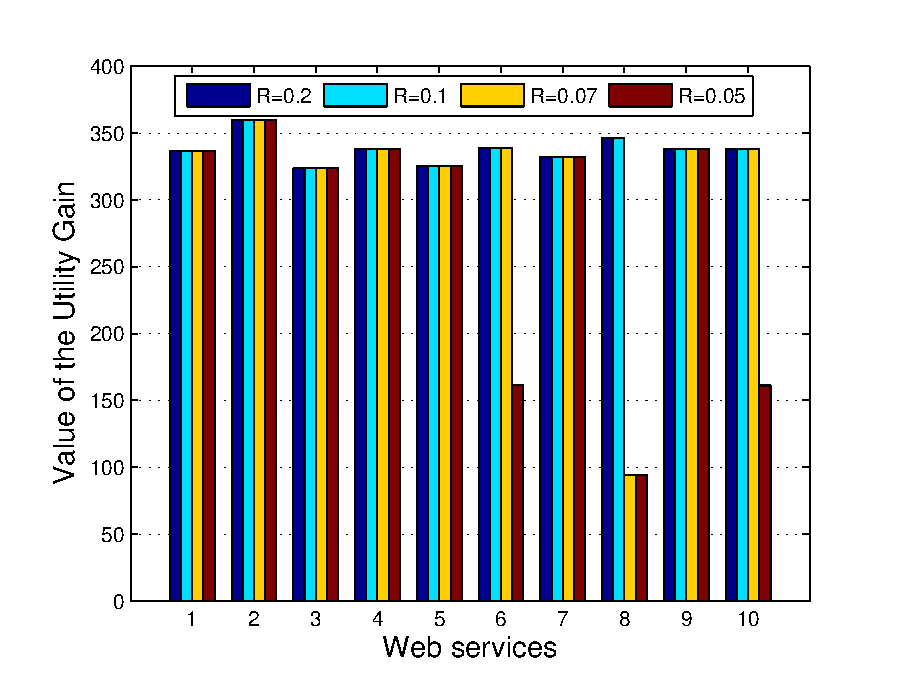
\includegraphics[width=3.5in]{figures/utility_gain_r.eps}
%\caption{DDM Utility Gain Value}
%\label{utility_gain_value}
%\end{figure}
%
%\begin{figure}%[!t]
%\centering
%\includegraphics[width=3.5in]{figures/utility_ratio_r.eps}
%\caption{DDM Utility Gain Ratio}
%\label{utility_gain_ratio}
%\end{figure}


The closest related work \cite{10.1109/TSC.2012.12,
DBLP:conf/IEEEscc/LimTMB12, DBLP:conf/IEEEscc/KhosravifarABT11} and our
previous work \cite{journal-community-formation} regarding the community formation problem have considered a centralized approach where a community manager has complete information of all the web services and their quality
metric and parameters. Those proposals run complex algorithms through all the space of
solutions in order to find the optimal answer. However, in this research work, we
have considered an unexplored and more realistic situation where information is incomplete and a decision
profile is generated based on a smaller set of web services. Our solution helps
communities and web services select actions that lead towards
maximizing their utilities. Therefore, considering the different settings,
we cannot experimentally compare our work with the mentioned related work.


To compare our work against a benchmark, we utilize the same communities and web services with a simple rational decision making mechanism in which a community will choose to join another one if it increases its utility by any amount, without aiming to be optimal. We call this method the {\textit{rational} method. We have chosen 10 random web services and compared the results with web services which adopted our DDM model. Figure \ref{utility_gain_mlisa_and_rational} shows the comparison of the end result of utility gain values. In 18 out of 40 tries, \emph{rational} agents were not able to improve their utility at all because the communities they chose rejected their request, most likely because they would not have increased the utility of the other communities if they had joined them. The results show that a long-term strategic decision mechanism is needed to satisfy all the services within communities. Figure \ref{utility_gain_mlisa_and_rational_ratio} shows the same results in terms of ratio of utility gain.

\begin{figure}%[!t]
\centering
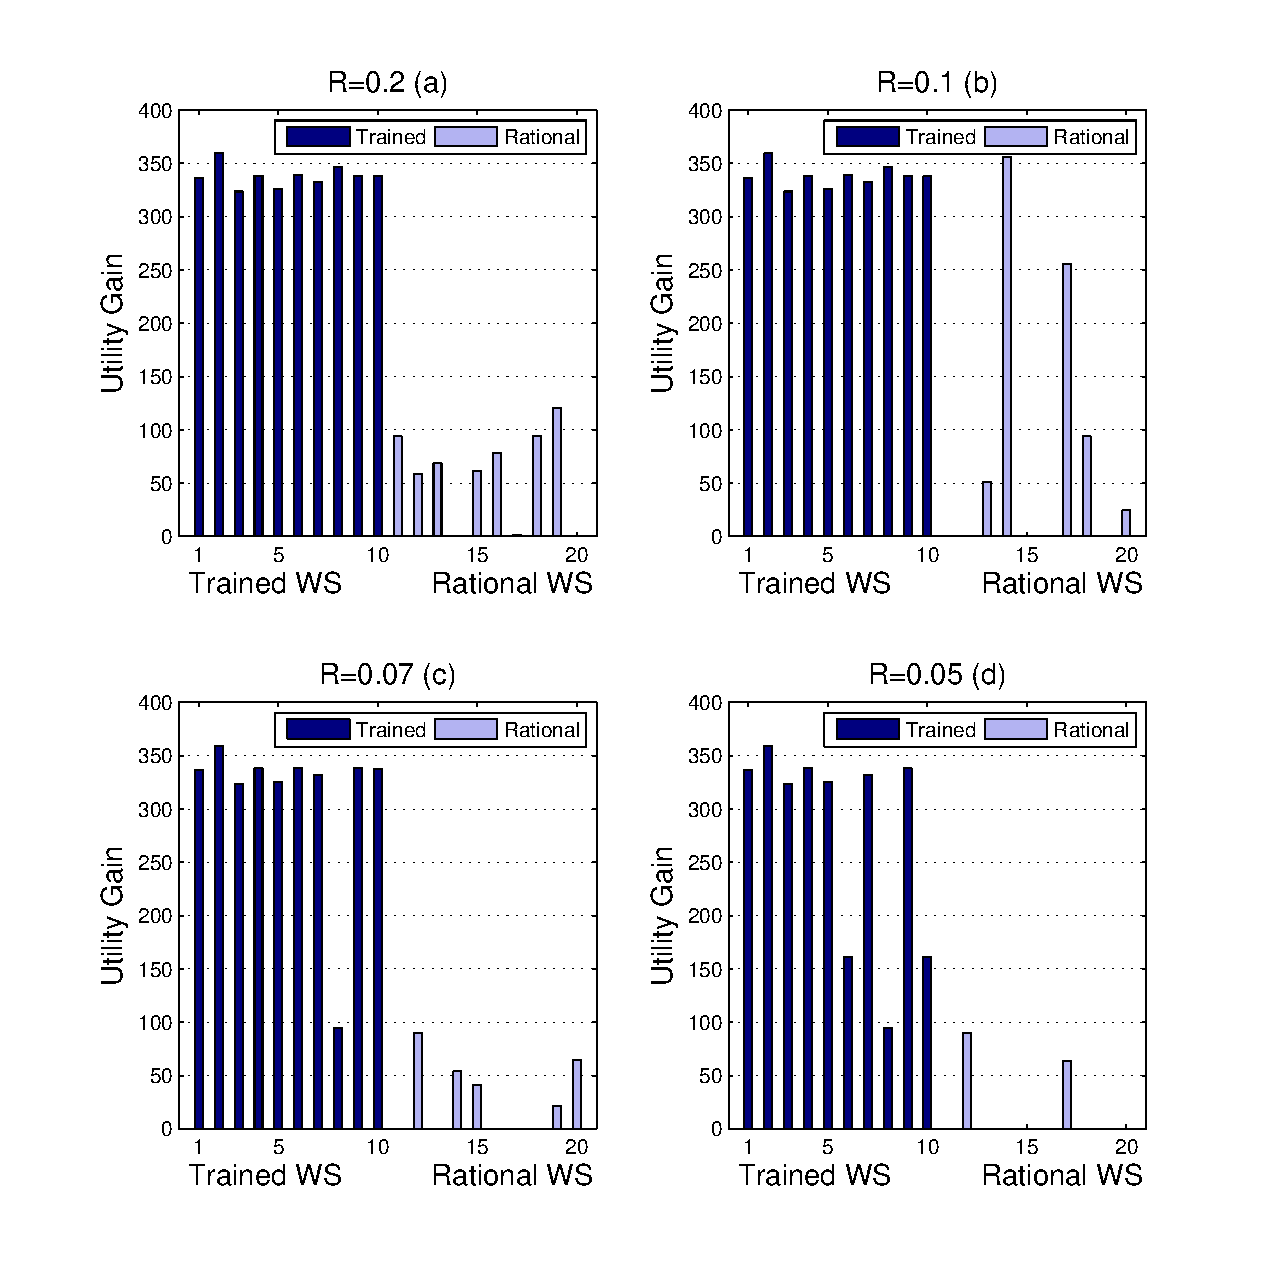
\includegraphics[width=3.5in]{figures/utility_gain.eps}
\caption{DDM against Rational: utility gain }
\label{utility_gain_mlisa_and_rational}
\end{figure}

\begin{figure}%[!t]
\centering
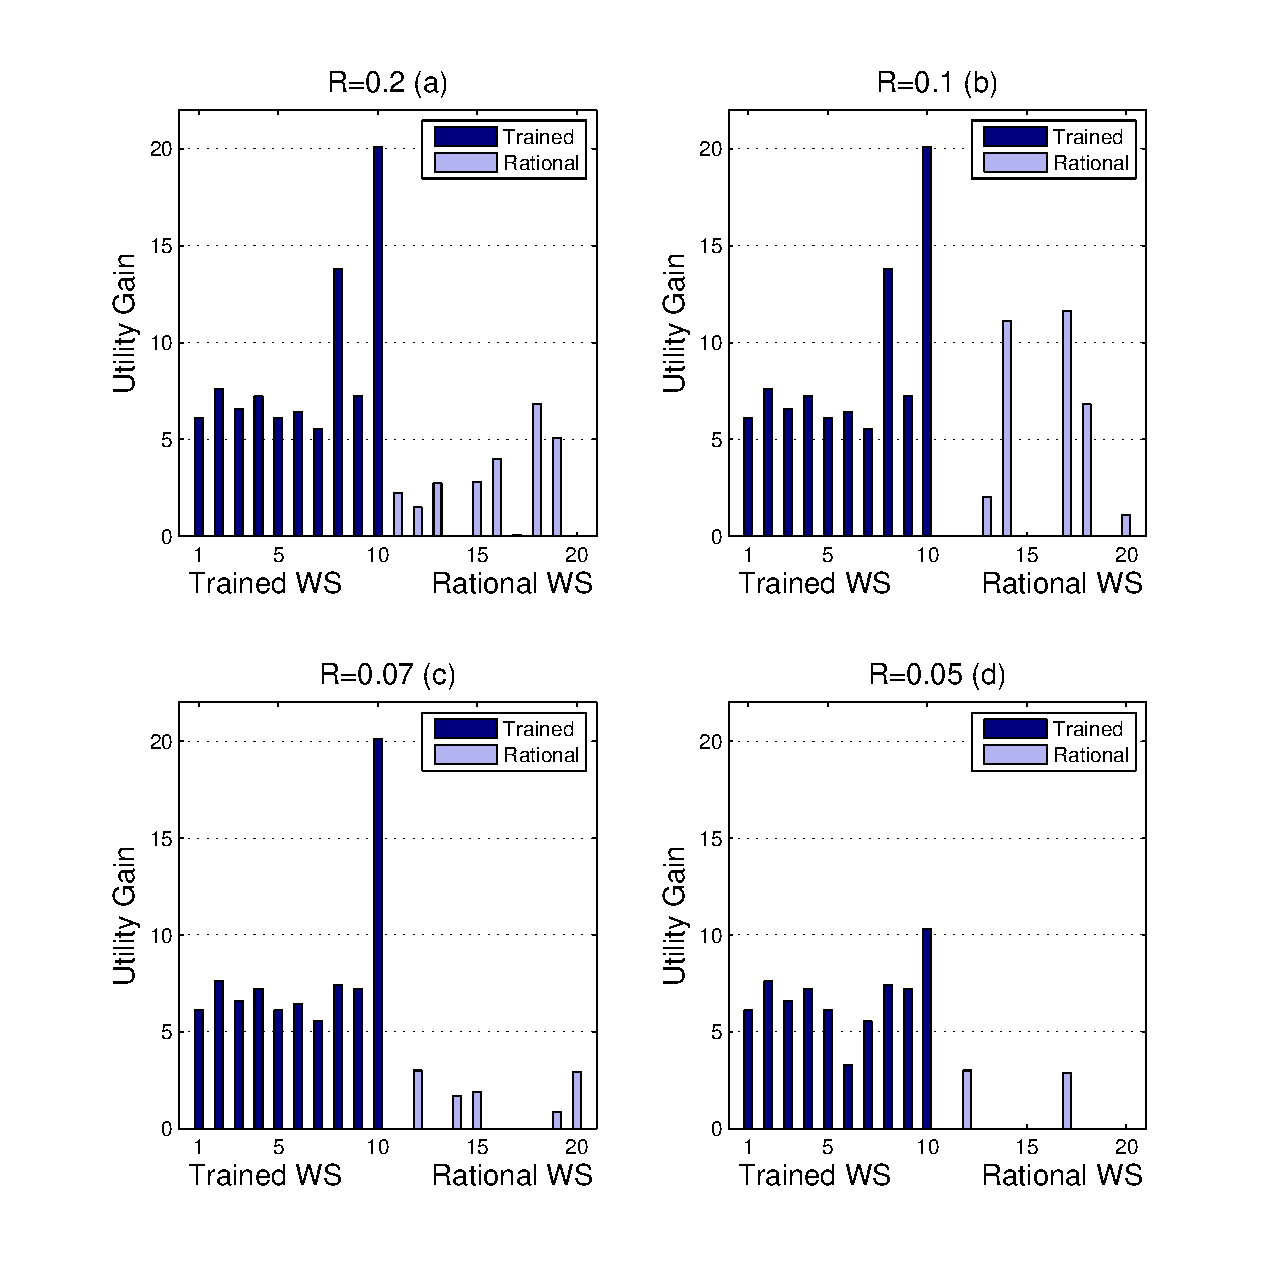
\includegraphics[width=3.5in]{figures/utility_ratio.eps}
\caption{DDM against Rational: ratio of utility gain}
\label{utility_gain_mlisa_and_rational_ratio}
\end{figure}

Now, we evaluate the performance of the decision profiles generated based on our data set for other communities.% which are not included in the decision tree creation process.
We create 1,000 communities from the web services in the data set that were not involved in the training process of our decision model. We define a distance function that measures the difference between basic features of communities, which measures the similarity among communities.

\begin{equation}\label{distance_c}
\begin{split}
distance (C_1, C_2) & = |Th_{C_1} - Th_{C_2}| \\
                    & + |A_{C_1} - A_{C_2}| + |Et_{C_1} - Et_{C_2}|
\end{split}
\end{equation}

Now, each community tries to find the closest community within the trained $CFVS$ set. Following its decision profile, the community can get a good estimate of the possible strategic decisions it can adopt. Basically, the trained profiles benefit the new communities in two ways. First, they provide the communities with a set of viable communities to join. Second, they provide an estimation of long-term utility gain for each available decision. In this experiment, we let communities follow the best decision within the decision tree provided to them.


In order to evaluate the performance of the mechanism, we used \emph{Receiver Operating Characteristic (ROC) curve}, which is a graphical plot illustrating the true negative rate against the false positive rate at various threshold settings in classifier systems. In order to classify our communities' selection strategies correctly, for each community, we evaluated the training process by replacing the community in the set with the closest one, from which it gets the strategy profile. If the actions are the same and the same utility levels are gained, we classify the decision as correct. Otherwise, it is classified as a wrong decision. \emph{AUC}, the area under the \emph{ROC curve}, is equal to the probability that a classifier will rank a randomly chosen positive instance higher than a randomly chosen negative one, and the higher the number the better the solution, which reflects better performance.  Figure \ref{roc5} illustrates the \emph{ROC curve} evaluation of the DDM decision making mechanism. As benchmark, we compare our method with two other methods: the \emph{rational} method and the \emph{greedy} method. The \emph{greedy} method only looks up the available list of communities and simply joins the community that maximizes its utility without considering any long-term strategy or other communities' acceptance scenarios. It is a greedy algorithm that focuses on choosing a locally optimal choice.

\begin{itemize}
  \item {\bf Rational Method:} Communities would send a join request to any available community, which will increase the utility. The other community would accept the join offer if its own utility gain is positive as well.
	\item {\bf Greedy Method:} Communities do a linear search among all the available communities and send a join request to the community which results in maximum utility. The other community would accept the join offer if its own utility gain is positive and the utility gain does not need to be the maximum for the community receiving the join request.
\end{itemize}

Figure \ref{roc5} compares the results for all the methods. The \emph{rational} and \emph{greedy} methods have very high failure rates compared to our method. Table \ref{fail_rate} illustrates the number of communities that failed to find the optimal collaboration group. The results support the need for a long-term training model in a successful decision making process.

\begin{figure}%[!t]
\centering
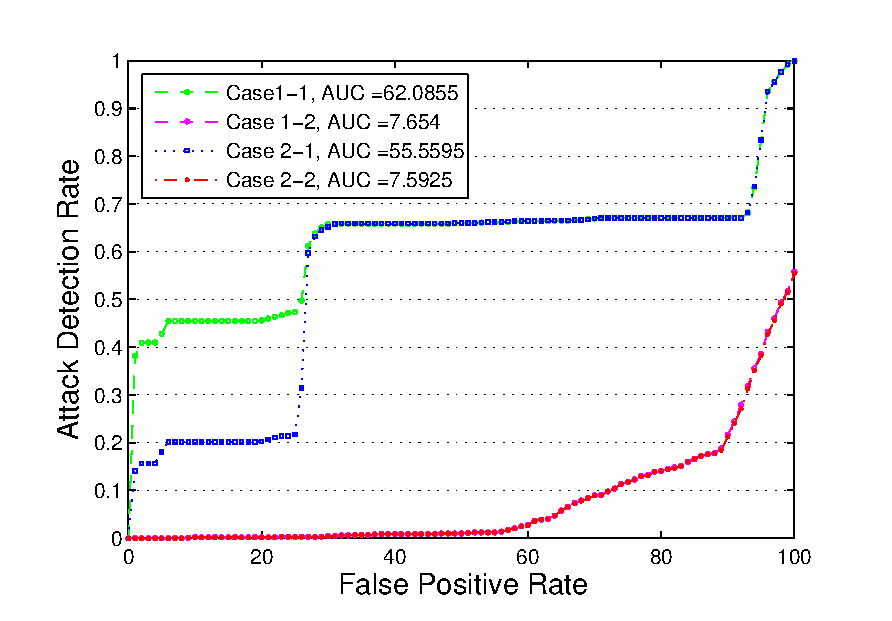
\includegraphics[width=3.5in]{figures/roc.eps}
\caption{RoC Curve}
\label{roc5}
\end{figure}

\begin{table}[ht]
\caption{Number of communities that misses the optimal decision, out of 1,000 communities} % title of Table
\centering % used for centering table
\begin{tabular}{|c|c|} % centered columns (4 columns)
\hline %inserts double horizontal lines
 Method&Miss \\ [0.5ex] % inserts table
%heading
\hline % inserts single horizontal line
 DDM r=0.05& 375 \\ % inserting body of the table
 DDM r=0.07& 137 \\
 DDM r=0.10& 6 \\
 DDM r=0.20& 6 \\
Rational Method& 717 \\
Greedy Method& 828 \\ [1ex] % [1ex] adds vertical space
\hline %inserts single line
\end{tabular}
\label{fail_rate} % is used to refer this table in the text
\end{table}


Now, we evaluate the system-specific results from users' and communities' perspectives. By distributing tasks among the communities over the 64 time frames, we evaluate the revenue for each community. Figure \ref{stats1} shows the overall revenue gain of communities using our method. Figure \ref{stats2} shows the momentarily revenue gain for each community in each time slot compared to the previous time. These results show that the run with the higher learning rate of $r=0.20$ starts discovering better communities to join much earlier. The runs with slow rates seem to find some communities to join initially, but then they slow down until later, when they start discovering new communities to join.


\begin{figure}%[!t]
\centering
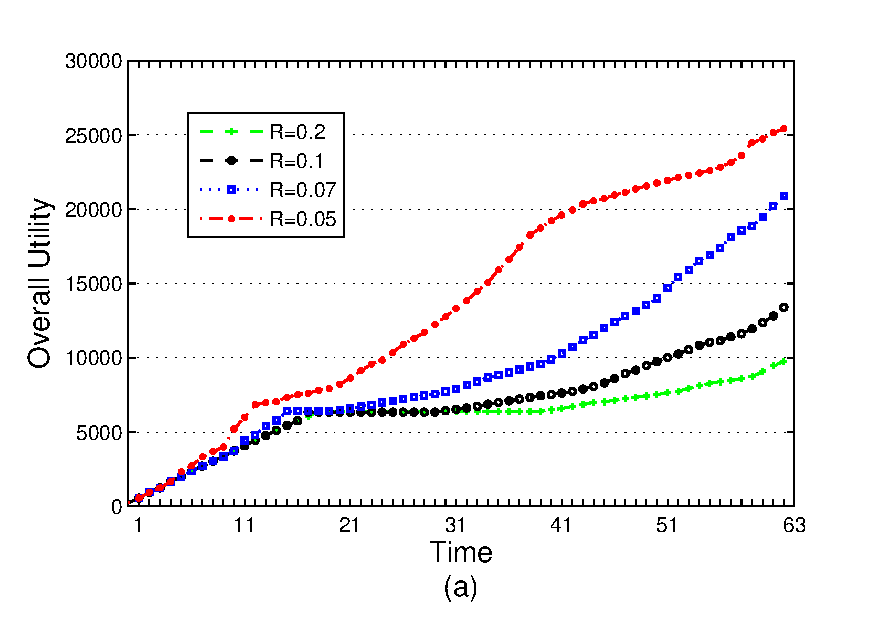
\includegraphics[width=3.5in]{figures/stats1.eps}
\caption{Overall utility of all the communities}
\label{stats1}
\end{figure}


\begin{figure}%[!t]
\centering
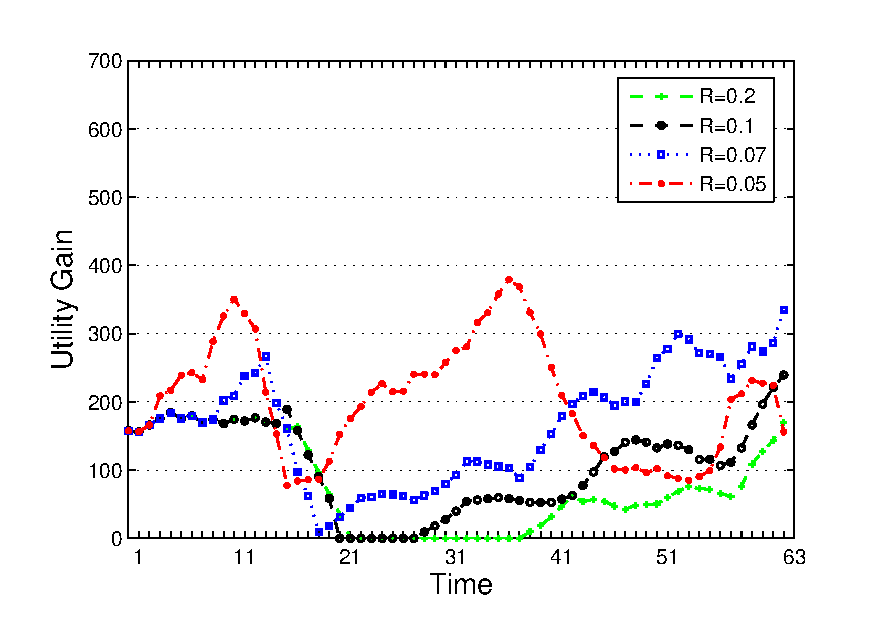
\includegraphics[width=3.5in]{figures/stats2.eps}
\caption{Utility gain over time}
\label{stats2}
\end{figure}

Figure \ref{stats3} depicts the average community size over time, which essentially represents the number of new communities being formed. The results show once again the communities using DDM with higher search rates grow faster in size, implying that the communities find appropriate web services to join with faster.

\begin{figure}%[!t]
\centering
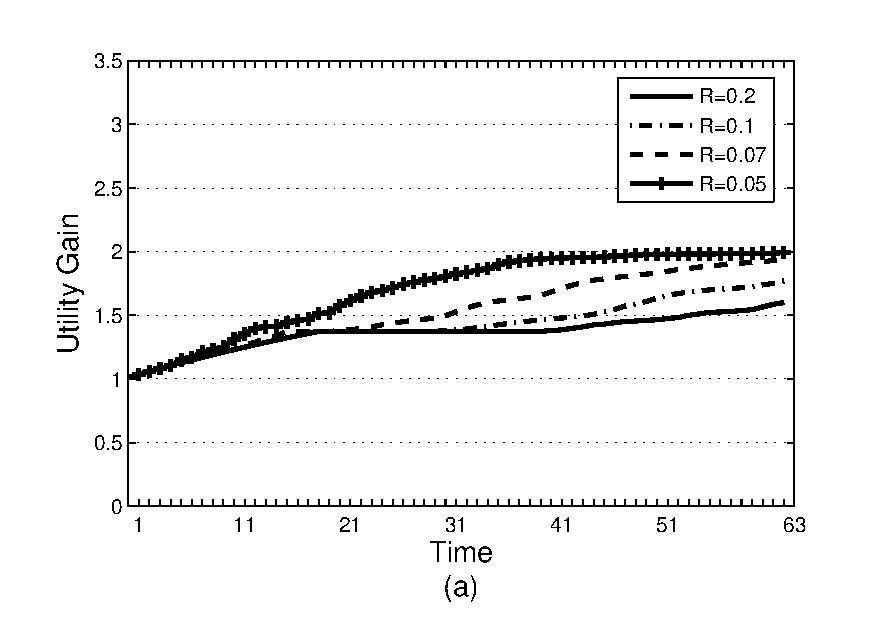
\includegraphics[width=3.5in]{figures/stats3.eps}
\caption{Average community size}
\label{stats3}
\end{figure}



\section{Related Work}\label{s:related_work}

Most of the recent work on communities of services are either
user-centric and focus on user satisfaction
\cite{Chun02user-centricperformance} or system-centric and focus
on the whole system throughput, performance and utilization. There
are many contributions in distributed, grid, cluster and cloud
services which are system-centric. However, in real world
environments and applications, both users and service providers
are self-interested agents, aiming to maximize their own profit.
In those environments, both parties (users and services) will
collaborate as long as they are getting more benefits and payoff.

In this direction, recently \cite{DBLP:conf/IEEEscc/LimTMB12,
DBLP:conf/IEEEscc/KhosravifarABT11, 10.1109/TSC.2012.12} proposed
mechanisms to help users and services maximize their gain. A
two-player non-cooperative game between web services and community
master was introduced in
\cite{DBLP:conf/IEEEscc/KhosravifarABT11}. In this game-theoretic
model, the strategies available to a web service when facing a new
community are requesting to join the community, accepting the
master's invitation to join the community, or refusing the
invitation to join. The set of strategies for communities are
inviting the web service or refusing the web service's join
request. Based on their capacity, market share and reputation, the
two players have different sets of utilities over the strategy
profiles of the game. The main limits of this game model are: 1)
its consideration of only three quality parameters, while the
other factors are simply ignored; and 2) the non-consideration of
the web services already residing within the community. The game
is only between the community master and the new web service, and
the inputs from all the other members and their influence on the
master's decision are simply ignored. The consideration of those
inputs and this influence factor is a significant issue as
existing web services can lose utility or payoff because of the
new member, which can result in an unhealthy and unstable group.
The problem comes from the fact that the existing members should
collaborate with the new web services, so probably their
performance as a group can suffer. Existing members may even
deviate and try to join other communities if they are unsatisfied.
Those considerations of forming stable and efficient coalitions
are the main contributions of our thesis.

In \cite{DBLP:conf/IEEEscc/LimTMB12}, a 3-way satisfaction approach
for selecting web services has been proposed. In this approach,
the authors proposed a web service selection process that the
community masters can use. The approach considers the efficiency
of all the three involved parties, namely users, web services and
communities. In this work, it is shown how the gains of these
parties are coupled together using a linear optimization process.
However, the optimization problem in this solution tends to
optimize some parameters considering all web services regardless
of their efficiency and contribution to the community's welfare.
Moreover, there are no clear thresholds for accepting or rejecting
new web services. The solution of the optimization problem could,
for instance, suggest web services already residing within the
community to increase or decrease their capacity to cover up the
weakness of other parties in the system. However, a high
performing web service could deviate anytime it finds itself
unsatisfied within the community instead of adjusting its service
parameters.

In \cite{10.1109/TSC.2012.12}, a cooperative scheme among
autonomous web services based on coalition game theory has been
introduced. The authors have proposed an interesting algorithm to
reach individually stable coalition partition for web services in
order to maximize their efficiency. The communities choose new web
services on the promise that it would benefit the community
without decreasing any other web service's income. In the proposed
model, the worth of community is evaluated with high emphasis on
the availability metric and considering price and cost values
only. The community structure is based on a coordination chain,
where a web service is considered as a \emph{primary} web service
and the community task-distribution method initially invokes the
primary web service and only if the primary web service is
unavailable, the method invokes the next backup web services as
they are ordered in the coordination chain. We believe that this
coordination chain limits the cooperation power as it introduces a
sort of hierarchy. However, in pure and open cooperative models,
such as the one we propose in this paper, active cooperation
activities engaging simultaneously many agents so that they can
perform the tasks more efficiently are being used. Moreover, if
the availability is high, which is the case nowadays with the
recent advancements in cloud infrastructures and hardware technologies, the
backup web services will end-up having a very low chance of
getting jobs, especially the ones further in the chain. This will
results in a considerable waste of web services capabilities.

All the proposed frameworks share a common aspect, which is providing the solution based on assumption of having complete information of all services and performing evaluations based on a large number of input each time they want to adopt a strategic decision making process.
So basically, these solutions generally suffer from high complexity, which makes decision making very hard, even impossible in some cases in a real-time fashion, or they simplify important aspects to make it practical in the real world, thereby hurting the decision making performance. We address this issue by introducing DDM a framework that operates based on a trained model that regulates web service agents' decision making process in terms of cooperating with one another. After being trained, web services get to compute expectations as utilities they would gain while cooperating with communities of different characteristics. Therefore, web services and communities can make prudent decisions when inviting a web service to join or accepting a join inquiry initiated from a web service. In general, DDM equips web services with efficient methods for foreseeing how their choices will impact their long-term and short-term goals; therefore, opting for best decision available. \\

\noindent \textbf{Web Service Communities}

Here we introduce the related research work regarding the engineering and formation of communities of web services. In \cite{DBLP:journals/internet/BenatallahSD03}, Benatallah et al. defined communities of web services as \emph{Service Containers} that aggregate substitutable web services having the same set of operations and providing common functionalities. They abstracted \emph{Service Containers} as web services that are created, advertised, discovered and invoked just as elementary web services. The \emph{Container} is considered as a manager that is responsible for web service selection upon receiving a request on run-time. The authors have proposed a scoring technique based on non-functional requirements of the request and web service capabilities to dynamically chose the web service to perform the requested task. A similar concept was proposed by Maamar et al. in \cite{DBLP:journals/ijebr/MaamarSTBB09}. The authors introduced web service communities as a collection of web services with a common functionality but different QoS properties. A community manager, upon receiving a request, delegates the request to one of its current members. The choice is based on the performance history and quality metrics of each web service. The authors have proposed an efficient global web service selection algorithm in order to approach quality constraints and preferences for composite services which requires aggregation of different types of services to satisfy the user. In the same line of research, Benslimane et al. \cite{Liris-2770} have proposed a multi-layer approach grouping similar web services into communities and having an interface implemented as an abstract web service for accessing the community. The considered layers are: composite, management and community. The interactions among those layers and the bindings are performed by a generic driver called Open Software Connectivity (OSC). However, unlike our work, these proposals only tackle the problem of internal community management from the task execution perspective, but not the problem of community formation and the one of dynamically selecting which community to join and which web service to invite. Moreover, the web services selection process is done centrally by the community manager, while we address the problem more realistically from the distributed angle.

In \cite{managing-hela-jalel}, Limam and Akaichi have proposed web
service communities with centralized access across distributed web
services. They have proposed a framework for web service
management, query resolution among communities and a query caching
mechanism executed by the manager to improve the performance of
query resolution process among many distributed communities. The
key idea is to cache previous computed results for answering
future queries. Maamar et al. initially in \cite{conf/webist/MaamarLBTS07} and
then comprehensively in \cite{DBLP:journals/ijebr/MaamarSTBB09}
proposed an architecture utilizing \emph{Contract-Net} protocol
for engineering task distribution within communities of web
services. The protocol is centrally executed by the community
manager. This architecture has been further extended in
\cite{CSTintercommunity, conf/IEEEscc/BenharrefSBB11,
conf/IEEEscc/KhosravifarBMMT10, conf/aina/LimTM11}. Two types of
roles have been distinguished for community members: masters and
slaves. Master web services are community managers that lead
communities and are responsible for membership management. They
can invite and convince slave web services to join the community,
and attract new slave web services to their communities by
awarding them better payoff. Moreover, they can eject some slave
members from the community to improve its overall reputation if
these members are misbehaving or cannot provide the promised QoS.
In \cite{Medjahed05adynamic}, Medjahed and Bouguettaya have
developed a community as a ``cluster'' that groups Web services
based on a specific area of interest. All web services in a given
community share the same functionality. These communities are
created by \emph{third party community providers} which use the
\emph{community ontology} as a template and define a set of
operations that all web services within a community should
provide. Using semantic analysis on web service operations, web
services either find and join a community with similar
functionality or create a new operation description for a new
community. The authors have described the concept of
\emph{community agents} associated to \emph{community providers}.
A community agent is responsible, among other things, of the
registration of services with the community. An example of a
community that provides health care services to senior citizens
has been used. In this example, a governmental entity is needed to
check the health care standards used by the members before
authorizing them to be part of the community. Such a central
entity is represented by the community agent. Thus, community
agents are playing the role of community managers. In a close work
\cite{Zeng:2003:QDW:775152.775211}, Zeng et al. have described a
global planning selection algorithm and a delegation algorithm to
be run when a request to execute an operation is received by the
community. This needs a central entity to run those algorithms.
Such entity plays the same role as the community coordinator or
manager. All these proposals have in common the consideration
of the central entity for community management, which includes the hiring and firing of the community members, while our approach is fully distributed. Moreover, the stability of the community has not been investigated. Another major difference with our work is that the decision making process is only one way and unilateral from the community manager perspective. In our contribution, both participants, namely communities and web services, participate in the decision making process and a joining decision is made only if it is the best option for both players.


%%%%%%%%%%%%%%%%%%%%%%%%%%%%%%%%%%%%%%%%%%%%%%%%%%%%%%%%%%%%%%%
\section{Summary}\label{sec:conclusion-cha4}

In this research work, we proposed a training model for the problem of membership management of communities of web services. Using the traning model we created a decision making profile for each community and web service involved which provides them with a set of feasible and utility increasing moves. This utilized our web services with efficient methods of foreseeing how their choices of actions would impact their long-term and short-term goals, therefore they opted for best decision available. The ultimate goal is to choose the best decision when it comes to communities formation, among many possible short-term rational and utility increasing choices. The experimental results show that our algorithms provide web services and community owners, in real-world-like environments, with applicable and near-perfect decision making mechanisms. The results of experiments using real data samples support the need for a long-term training model in a successful decision making process.

Our plan for future work is to advance learning process on the training set that we provided in our work. SVN machine learning algorithm are suitable in classification of our training data set, to better classify correct or wrong decisions based on long-term utility gains, as data set outputs. This can further facilitate the process of finding optimal cooperators in regards to enhancing web services' overall performance as service providers.

In next chapter, we analyse the internal community behaviour of web services, and propose a model for competing and cooperating agents within the communities of web services.



%%%%%%%%%%%%%%%%%%%%%%%%%%%%%%%%%%%%%%%%%%%%%%%%%%%%%%%%%%%%%%%%%%%%%%%%%%%%%%%
%% Chapter 5 : Probabilistic Group Social Commitments.
%%%%%%%%%%%%%%%%%%%%%%%%%%%%%%%%%%%%%%%%%%%%%%%%%%%%%%%%%%%%%%%%%%%%%%%%%%%%%%%
\chapter{On Probabilistic Group Social Commitments}\label{cha:PCTLKC+}

In this chapter\footnote{Part of the results presented in this chapter, namely PCTL$^{\textrm{kc+}}$ logic, has been published in SoMet\_14 \cite{Sultan2014c}. The results of model checking PCTL$^{\textrm{kc+}}$ have been sumbitted to the Engineering Applications of Artificial Intelligence journal \cite{Sultan2014d}}, we improve and extend the work presented in Chapter \ref{cha:PCTLKC} by refining the probabilistic logic of knowledge and commitment (PCTL$^{kc}$) and then extending the refined logic further by operators for group knowledge and group commitment. In this respect, we define a semantics for the group social commitment operator and integrate it into the resulting logic. The developed logic is called the new probabilistic logic of knowledge and commitment (PCTL$^{\textrm{kc+}}$). Finally, we introduce a new formal verification technique that considers the new group modalities and implement it on top of the PRISM model checker.


\section{Introduction} \label{Introduction}

One of the major challenges in building complex software products
such as Multi-Agent Systems (MASs) is to advance error detection
at early stages of their life-cycles. %The social context of interacting agents in MASs has gained significance recently.
MASs community has witnessed an important shift in defining the semantics of ACLs from the so-called mental approaches that is hard to verify \cite{Singh2000} to social approaches which exploit observable and verifiable social commitments. However, the increasing demand to use social commitments as a means of communication among interacting parties \cite{Baldoni2014,Chesani2013,Akin2013} requires reasoning about and verifying the relationship between social commitments and some other systems' aspects such as agents' knowledge and uncertainty especially in the case of having group-commitment scenarios. In addition to verifying the interactions between social commitments and knowledge in the presence of uncertainty, the ultimate objective of this chapter is to verify the interactions between the two elements when the scope of interacting agents goes beyond the common agent-to-agent (i.e., one-to-one) scheme.

In order to effectively capture and express the interactions between individual and group social commitments and knowledge in probabilistic MASs, we propose a new modal logic called the new probabilistic logic of knowledge and commitments PCTL$^{\textrm{kc+}}$ which is built by combining a consistent logic of knowledge and commitment CTLKC$^+$ \cite{Al-Saqqar2014a} with a well established probabilistic temporal logic PCTL \cite{Hansson1994}. The resulting logic is extended further to accommodate operators for the group knowledge and group commitments.

At present, there is a relatively large gap in addressing the
concepts of knowledge and social commitments simultaneously in
MASs, especially with the presence of uncertainty. Existing
approaches that address the interaction between knowledge and
social commitments either limit the scope of interacting
agents to the widely used one-to-one commitment scheme and ignore the uncertainty aspect of MASs \cite{Al-Saqqar2014a}, or adopt a different kind of commitments called ``internal commitment'' rather than the ``social commitments'' that we consider in this thesis \cite{Schmidt2004}.
Furthermore, although the notion of ``group'' is important in the multi-agent community \cite{Sanchez-Anguix2013,YuW2010}, group social
commitments has not been formalized and verified yet. As knowledge
and social commitments influence each other in many real world
applications \cite{Al-Saqqar2014a}, their interactions need to be
reasoned about and verified in a systematic manner. As we said before,
uncertainty in MASs may arise due to imperfect information about
the environment in which agents interact. Besides, in some situations, it happens that even if there is some state of affairs (i.e., content of a commitment) that an agent wants to bring about, its actions might not reliably drive the state of affairs into the desired state \cite{Sultan2014a}. Consequently, commitments themselves become stochastic and the degree to which the commitment can be satisfied is not always
guaranteed.

To motivate our study of representing and verifying the
interaction between individual and group knowledge and social
commitments in probabilistic MASs when taking into account
one-to-many commitments, let us consider the following simple
example. A professor teaching an engineering course with a
capacity of $20$ students. Various scenarios could happen within
this context.

\begin{itemize}
\item \verb"Scenario 1": while the professor was explaining some
new concepts in the course, one of the students asked the
professor to provide him with more material regarding these
concepts. The professor then promised to email the student some
references the next day. This promise can be considered as a
commitment from the professor towards the student to provide him
with extra material for the new concepts. \item \verb"Scenario 2":
in the lecture before the mid-term exam, students requested the
professor to exclude some material and shorten the duration of the
exam accordingly. At the end of the lecture, the professor agreed
to exclude some parts of the covered material and to make the exam
one hour long.  This agreement can be considered as a commitment
from the professor to the group of students who are registered in
this course. Right after the class, the professor posted in the
course web site an update confirming what they agreed on.
\end{itemize}
In the first scenario, obviously both the professor and student
are aware of the commitment (sending extra materiel). However, in
the second scenario, every student registered in the course, and
not necessarily present during the lecture,  has to know about
this agreement (commitment) to avoid wasting time studying
excluded parts. In fact, because of some unexpected factors like
absence of the professor on the day of the exam, email delivery
failure, power outage, etc, there is no guarantee that these
commitments are  going to be surely fulfilled. Therefore, it is
important to have a logic system with the ability to not only
express the interaction between knowledge and social commitments,
but also to handle the concepts of knowledge and commitments
within the scope of a group when uncertainty matters. Once such a
logic is defined, it can be invested as the underlying logic for a
verification technique to verify some desirable and useful
properties expressing combinations of knowledge and social
commitments under uncertainty.

The work presented in this chapter can be seen as extension and continuation of the work presented in Chapter \ref{cha:PCTLKC} where reasoning about and verifying interactions between individual knowledge and social commitments in probabilistic MASs were first introduced. In Chapter \ref{cha:PCTLKC}, we proposed a probabilistic logic called PCTL$^{kc}$ whose expressiveness power allowed us to formulate combinations of the two concepts in the presence of uncertainty. PCTL$^{kc}$ logic was built by fusing two logics, namely PCTLC \cite{Sultan2013} and PCTLK \cite{Wan2013} using the
independent join technique \cite{Franceschet2004}. However, as pointed out in \cite{Al-Saqqar2014a}, the social accessibility relations given in \cite{Bentahar2012,El-Menshawy2013a}, have an over-specification problem, and consequently the PCTL$^{kc}$ logic suffers from some paradoxes as it adopts the aforementioned accessibility relations.

To elaborate, there exist some situations that are not desirable in real settings but with the use of PCTL$^{kc}$, they are valid. One major problem in PCTL$^{kc}$ is that agents commit everything they know to others, which brings the lack of privacy into being. Formally, this is represented by the following postulate:

\begin{itemize}
\item $K_i \varphi \Rightarrow C_{i \rightarrow j}\varphi$,  where $i \neq j$.
\end{itemize}

The validity of this postulate is based on the fact that by
establishing communication channels through which commitments are
supposed to be exchanged, the epistemic relation needed to define
the semantics of knowledge is also established. This is not
reasonable in open environments where agents are selfish. Another
problem is that agents commit everything known by others. That is,
when an agent knows that another agent knows something, the first
agent commits to bring about what the other agent knows, formally:

\begin{itemize}
\item $ K_i K_j \varphi \Rightarrow C_{i \rightarrow j} \varphi$ where $ i \neq j$.
\end{itemize}

Such a postulate should be avoided in MASs because it is not
realistic for an agent to commit for something that is out of its
capabilities. Moreover, this postulate can result in serious
circumstances if agent $j$ is malicious, so it can express
incorrect knowledge about the other agent, obliging it to
establish unwanted commitment.

On the other hand, we have some reasonable situations that should
be always valid but with the use of PCTL$^{kc}$ they can be
unsatisfied. One example in this respect is when agents should be always aware about the fulfillment of their own commitments.

\begin{itemize}
\item $Fu(C _{i\rightarrow j} \varphi) \Rightarrow K_i Fu(C
_{i\rightarrow j} \varphi)$ where $i \neq j$
\end{itemize}

It is realistic for this postulate to be valid because any agent should be aware of its fulfillment actions in order to prevent fulfilling the same commitment again and again. However, this postulate is not valid in PCTL$^{kc}$ because of the same reasons mentioned earlier. Consequently, PCTL$^{kc}$ fails to efficiently handle some practical situations in which knowledge and social commitments need to interact.

The problem is that one of the underlying logics of PCTL$^{kc}$, which
is PCTLC \cite{Sultan2013}, is built using the social accessibility relations given in \cite{Bentahar2012,El-Menshawy2013a}, which in fact over specifies and over constrains the concept of illocutionary communication. In a recent work, Al-Saqqar et al. \cite{Al-Saqqar2014a} have figured out that although the social accessibilities presented in \cite{Bentahar2012,El-Menshawy2013a} function perfectly when the concern is to model social commitments independently, they have some limitations when combined with the epistemic accessibility relations in the same model. The authors in \cite{Al-Saqqar2014a} modified the social accessibility relations proposed in \cite{Bentahar2012,El-Menshawy2013a} in order to prevent the unintended emergence of the epistemic accessibility relations from the social accessibility relations when the two accessibilities combined in the same model. Technically speaking, they relaxed the conditions upon which the social accessibility relations are established in order to decouple the social accessibility relations from the epistemic accessibility relations. The new definition of social accessibilities does no longer depend on the unshared variables but rather depends merely on the shared variables between the interacting agents as discussed in Chapter \ref{cha:background}. The new condition upon which a communication channel is established is stated below:

 $ s \approx_{i \rightarrow j} s' $ iff $ Var_i \cap Var_j \neq \emptyset $ such that $ \forall x \in Var_i \cap Var_j $ we have $ l_i^x(s) =
l_i^x(s') = l_j^x(s')$, where $\approx_{i\rightarrow j} \subseteq S \times S$ is the social accessibility relation. It has been proven that with the new social accessibilities, the resulting logic is consistent \cite{Al-Saqqar2014a}.

The work presented in this chapter differs from the one proposed in Chapter \ref{cha:PCTLKC} in the following points:

\begin{enumerate}
\item While the logic presented in Chapter \ref{cha:PCTLKC} suffers from
some paradoxes, the current work builds upon a consistent logic of
knowledge and commitment CTLKC$^+$ \cite{Al-Saqqar2014a} which
ensures having a paradox-free logic.

\item The new logic allows us to reason about commitments among
multiple agents instead of limiting the scope to merely two
agents. The concept of group knowledge is also integrated to the framework allowing us to reason about the knowledge in the case of group of agents.

\item In the current work, we generalize the model checking
technique that has been proposed in Chapter \ref{cha:PCTLKC} to fit the new group commitment operators as well.
\end{enumerate}


The contributions of this chapter are threefold. First, we present a new probabilistic logic called (PCTL$^{\textrm{kc+}}$) with expressiveness abilities to capture and represent the interactions between individual and group knowledge and social commitments.
Second, we introduce a formal verification technique for the probabilistic logic PCTL$^{\textrm{kc+}}$. The proposed technique is based on reducing
the problem of model checking PCTL$^{\textrm{kc+}}$ to the problem
of model checking PCTL. This is achieved through 1) advocating a
set of transformation rules that transform the
PCTL$^{\textrm{kc+}}$ model into a Markov Decision Process (MDP),
and then converting the obtained MDP into a DTMC using the notion
of ``adversary'' \cite{Forejt2011}; 2) reducing
PCTL$^{\textrm{kc+}}$ formulae into PCTL formulae based on a set
of formal reduction rules. Third, we implement our reduction model checking
technique on top of PRISM and apply it on a concrete case study,
namely the online shopping system \cite{Gomaa2011}. We then check
some system's properties written as PCTL$^{\textrm{kc+}}$ formulae
using the PRISM model checker by checking their corresponding PCTL
formulae. Figure \ref{fig:approach-PCTLKC+} depicts a schematic
view of our proposed framework.


\begin{figure}[t]
                \begin{center}
                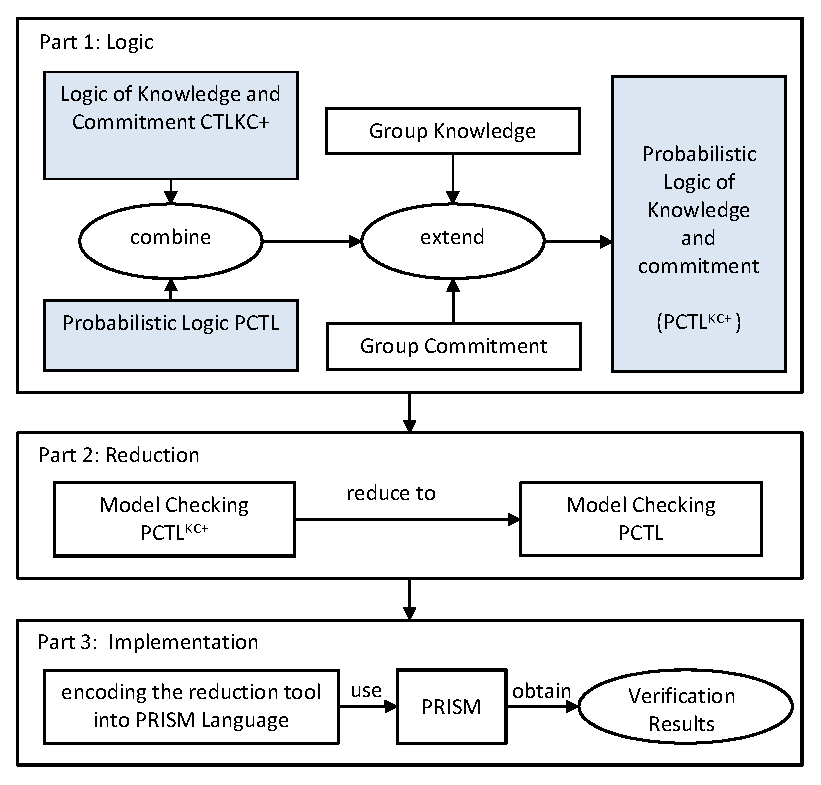
\includegraphics[width=14cm, height=10cm]{chap5/img/approach-cha5-new.eps}
                \end{center}
                \caption{A schematic view of the probabilistic group social commitment approach} \label{fig:approach-PCTLKC+}
                \label{Stack}
                \end{figure}



\section{The New Probabilistic Logic of knowledge and Commitment (PCTL$^{\textrm{kc+}}$)} \label{sec:logic}

To overcome the inconsistency problem of PCTL$^{kc}$, we develop a new logic called the new probabilistic logic of knowledge and commitment (PCTL$^{\textrm{kc+}}$). To build PCTL$^{\textrm{kc+}}$, there are two obvious resources available in the literature: 1) the traditional temporal logics that have been developed for knowledge and social commitments independently or together such as CTLC \cite{Bentahar2012}, CTLK \cite{Lomuscio2007}, and CLTKC$^+$ \cite{Al-Saqqar2014a}; and 2) the existing probabilistic logics available in the literature such as PCTL \cite{Hansson1994}, PCLTK \cite{Wan2013}, and PCTLC \cite{Sultan2014a}. Unfortunately, none of these resources is perfectly suitable for the task. The former resource neglects the uncertainty aspects in MASs, while the
latter doesn't capture the interaction between knowledge and
social commitments. Therefore, we propose a solution that draws
upon both resources. In particular, we combine an existing
consistent logic of knowledge and commitment CTLKC$^+$
\cite{Al-Saqqar2014a} with a well established probabilistic
temporal logic PCTL \cite{Hansson1994}. Then, we extend the
resulting combined logic by adding new operators for the group knowledge
and group commitment.

Before going further, let us first describe a new probabilistic model over which PCTL$^{\textrm{kc+}}$ formulae can be interpreted. This model is an extension of the formalism of interpreted systems
\cite{Fagin1995} with the concepts of epistemic accessibility and
social accessibility relations. Concretely, the model of PCTL$^{\textrm{kc+}}$ is generated from combining two extended versions of the interpreted systems formalism. These extended formalisms are the extended version introduced in \cite{Halpern2003,Wan2013} and a modified version of the extended version given in \cite{Bentahar2012,El-Menshawy2013a} due to Al-Saqqar et al. \cite{Al-Saqqar2014a}.


\begin{definition} [PCTL$^{\textrm{kc+}}$ Model] ~\label{dfn:Models}

\noindent Given a set of atomic propositions $\Phi_p = (p,q,r, \ldots)$ and a set of agents $\texttt{Agt}=\{1,\ldots,n\}$,  the model $\mathfrak{M_3}=(S,\textbf{P},I,\sim_1, \ldots
,\sim_n,\{\approx_{i \rightarrow j}\}_{{(i,j)}\in \texttt{Agt}^2},\nu)$ is a tuple where:
%
\begin{itemize}
\item  $S \subseteq L_1 \times \ldots \times L_n$ is a countable set of all reachable global states of the system. A state $s$ is reachable iff there exists a sequence of transitions from an initial state to $s$ in which the probability of each transition is greater than $0$.

\item  $I \in S$ is an initial global state for the system.


\item  $\textbf{P}:S\times S\rightarrow [0,1]$ is a total transition probability function defined as $\textbf{P}(s, s')=\tau(s,a^{s \rightarrow s'}, s')$ iff there exists a joint action $a=(a_1,\ldots,a_n) \in ACT$ such that\\
     $\sum_{i \in \texttt{Agt}} \tau_i(l_i(s),a^{l_i(s)\rightarrow l_i(s')},l_i(s')) > 0$ and $\sum_{s' \in S} \textbf{P}(s,s') =1$ for all $s \in S$.

\item  $\sim_i \subseteq S \times S$ is the epistemic accessibility relation for the agent $i$, such that for two global states $s$ and $s'$, we have: $s \sim_i s'$ iff $l_i(s)=l_i(s')$.

\item For each pair $(i,j) \in \texttt{Agt}^2$, $\approx_{i\rightarrow j} \subseteq S \times S$ is the social accessibility relation which is defined as follows: $ s \approx_{i\rightarrow j} s' $ iff $ Var_i \cap Var_j \neq \emptyset $ such that $ \forall x \in Var_i \cap Var_j $ we have $ l_i^x(s) = l_i^x(s') = l_j^x(s')$.

\item  $\nu : S \rightarrow 2 ^{\Phi_p} $ is a valuation function.

\end{itemize}
\end{definition}
%

The new model $\mathfrak{M_3}$ differs from the model $\mathfrak{M_2}$,  presented in Chapter \ref{cha:PCTLKC}, in one particular point which is the social accessability relation. While $\mathfrak{M_2}$ uses the social accessibility relation $\sim_{i\rightarrow j}$ that has been introduced in \cite{Bentahar2012,El-Menshawy2013a}, the new model adopts the one $\approx_{i\rightarrow j}$ proposed in \cite{Al-Saqqar2014a} in order to overcome the over-specification problem appeared in $\sim_{i\rightarrow j}$.



\subsection{Syntax of PCTL$^{\textrm{kc+}}$} \label{def:syntax-PCTLKC+}

\begin{definition}[PCTL$^{\textrm{kc+}}$ syntax]\label{def:syntax-PCTLKC+}
Let $\Phi_p=\{p,q, \dots\}$ be a set of atomic propositions, and $\texttt{Agt}=\{1, \dots, n\}$ be a set of agents. The syntax of PCTL$^{\textrm{kc+}}$, which is a combination of PCTLK \cite{Wan2013} and PCTLC \cite{Sultan2014a,Sultan2013} augmented with further operators for the group knowledge, is given by the following grammar:

\vspace{-0.5cm}
\begin{align*}
    \varphi & ::= p~|~\neg \varphi~|~\varphi \vee \varphi~|~\mathcal{K}~|~\mathcal{C}~|~ \mathbb{P}_{\bowtie k} (\psi)~|~\mathbb{P}_{\bowtie k}(\mathcal{K})|~\mathbb{P}_{\bowtie k}(\mathcal{C})\\
    \psi & ::=\bigcirc \varphi ~ | ~ \varphi ~U~ \varphi~|~ \varphi~ U^{\leq m} ~ \varphi \\
    \mathcal{K} & ::= K_i ~\varphi ~|~ E_{G} ~\varphi\\
    \mathcal{C} & ::= C_{i\rightarrow j} ~\varphi ~| ~ C_{i\rightarrow G} ~\varphi ~| ~Fu(C_{i\rightarrow j} ~\varphi) ~| ~Fu(C_{i\rightarrow G} ~\varphi)
\end{align*}
%
where;\\
\noindent -- $p\in\Phi_p$ is an atomic proposition\\
\noindent -- $i,j \in \texttt{Agt}$.\\
\noindent -- $G\subseteq \texttt{Agt}$.\\
\noindent -- $\mathbb{P}_{\bowtie k}$ is a probabilistic operator and $\bowtie \in\{<,\leq,>,\ge\}$.\\
\noindent -- $k\in [0,1]$ is a probability bound or threshold.\\
$m \in\mathbb{N}^+ $ is a positive integer number reflecting the maximum number of transitions needed to reach a certain state.\\
\noindent -- The Boolean connectives $\neg$ and $\vee$ are defined in the usual way.\\
\noindent -- $\varphi$ and $\psi$ are state and path formulae interpreted over the states and paths of $\mathfrak{M_3}$ respectively.\\
\noindent -- The modal connectives $\mathcal{K}$ and $\mathcal{C}$ stand for ``epistemic" and ``social" operators, respectively.\\

\end{definition}
\vspace{-0.5cm}

\noindent In this logic, formulae $\mathcal{K}$ are state formulae and used to express the epistemic properties through the operators; $K_i$ which stands for agent $i$ knows, $E_G$ which stands for everyone knows. Modal connectives $C_{i\rightarrow j}$ and $C_{i\rightarrow G}$ are called social formulae and stand for ``commitment'' from a debtor towards a single creditor, and ``commitment'' from a debtor to a group of creditors, respectively. Likewise, modal connectives $Fu(C_{i\rightarrow j})$ and $Fu(C_{i\rightarrow G})$ stand for ``fulfillment'' of the commitment $C_{i\rightarrow j}$ and ``fulfillment'' of the commitment $C_{i\rightarrow G}$, respectively. $\bigcirc, U$ and $U^{\leq m}$ stand for ``next time'', ``until'' and ``bounded until'' path modal connectives respectively.

%%%%%%%%%%%%%%%%%%%%%%%%%%%%%%%%%%%%%%%%%%%%%%%%%%%%%%%%%%%%%%%%%%%%%%%%%%%%%
%%%%%%%%%%%%%%%%%%%%%%%%%%%%%%%%%%%%%%%%%%%%%%%%%%%%%%%%%%%%%%%%%%%%%%%%%%%%%


\subsection{Social Commitments Classification} \label{sec:commitment-classification}



Social commitments for agent communication have been always looked
at within the scope of one-to-one. However,
back to our motivating example, we realize that in addition to the
usual agent-to-agent scheme, there are certain situations where
group-agent commitments are needed. In this chapter, we are
interested to move beyond the scope of one-to-one and
investigate the case of committing to multiple agents. The idea of
investigating other schemes of social commitments rather than the
one-to-one commitment scheme seems to be both technically
interesting and intuitively appealing. In what follows, we
distinguish between two different flavors of social commitments,
namely basic (or individual) social commitment and group social
commitment.

\begin{definition} [Basic Social Commitment]~

A basic social commitment is an agreement between two agents
namely, \texttt{debtor} and \texttt{creditor} such that the
\texttt{debtor} engages towards the \texttt{creditor} to bring
about a certain property.
\end{definition}

This is the simplest form of social commitments and has long been
investigated in the literature. The commitment in this case can be
represented using the following operator: $C_{i\to j} ~\varphi$
where $i$ denotes the debtor, $j$ denotes the creditor, and
$\varphi$ denotes the content of the commitment. The fulfillment
of such a commitment is written as follows: $Fu(C_{i\to j}
~\varphi)$. However, as the common form of social commitments is
the basic social commitment, we can simply use ``social
commitments" to refer to ``basic (or individual) social
commitments".


\begin{definition} [Group Social Commitment]~

A group social commitment is an agreement between a
\texttt{debtor} and a group of \texttt{creditors} to bring about a
certain property.
\end{definition}

This kind of commitments indicates the involvement of multiple
agents in the same commitment. The creditor is a group of
independent agents that join together as a single party due to
their shared interests in the commitment at hand. A group social
commitment is represented using the following notation: $C_{i\to
G} ~\varphi$, where $i$ denotes the debtor, $G$ denotes a group of
creditors, and $\varphi$ denotes the content of the commitment.
The fulfillment of such a commitment is given by the notation
$Fu(C_{i\to G} ~\varphi)$. Technically, a group social commitment
can be seen as the conjunction of individual basic social
commitments from the debtor $i$ to each agent in the group of
creditors $G$. Formally, $C_{i\to G} ~\varphi \equiv
\bigwedge\limits_{j\in G} C_{i\rightarrow j} ~\varphi$. An
intuitive explanation of the operator $C_{i\to G} ~\varphi$ is as
follows: for a group social commitment to be held at a certain
state, the content of the commitment must be true at every
accessible state from the commitment state with respect to the
group. This implies that none of the group members could be
excluded from having all accessible states satisfy the content of
the commitment. Consequently, it is obvious that for a state to be
socially accessible from the commitment state with respect to the
group, it has to be socially accessible with respect to at least
one of the agents of the group. Therefore, we resolve the
accessibility problem resulted from having group commitments by
taking the union of the social accessibility relations of each
single agent in the group. This in turn leads us to define the
group social accessibility relation based on the social
accessibility relations presented in Definition \ref{dfn:Models}.


Let $G\subseteq \texttt{Agt}$ be a group of agents. We define the group social accessibility relation from the social accessibility relation $\approx_{i \to j}$ as follows:
\begin{definition} [Social Accessibility Relations for Group Social Commitment] \label{dfn: group social
relations}~
%
\begin{itemize}

\item $\approx_{i \rightarrow G}$ is the union of the social accessibility relations between agent $i$ and each agent in the group $G$: $\approx_{i \to G}=\bigcup\limits_{j \in G}\approx_{i\to j}$.

\end{itemize}

\end{definition}


\begin{figure}[t]
                \begin{center}
                \includegraphics[width=7cm, height=5cm]{chap5/img/group-sc.eps}
                \end{center}
                \caption{Accessibility relations for group social commitment} \label{fig:group-sc}
                \end{figure}

Notice that group social commitments have all the properties of basic social commitments with an additional constraint that they can involve more than two agents. However, a group social commitment involving only two agents is equivalent to the basic social commitment. Figure \ref{fig:group-sc} depicts the idea of group social accessibility ($G=\{j_1, j_2\}$).

\subsection{Group Knowledge}  \label{sec:Group Knowledge}
In this work, we limit the scope of group knowledge to the concept of ``Everyone Knows" introduced in \cite{Fagin1995}. ``Everyone Knows" is denoted by $E_G ~\varphi$ and means that everyone in the group $G$ knows $\varphi$. Technically, ``Everyone knows" can be seen as the conjunction of the individual knowledge of each agent in the group. Formally, $E_G ~\varphi \equiv \bigwedge\limits_{i\in G} K_i ~\varphi$.

Before we proceed to present the semantics of
PCTL$^{\textrm{kc+}}$, we need to define the epistemic
accessibility relation for $E_G ~\varphi$. Let $G\subseteq
\texttt{Agt}$ be a group of agents. We define the epistemic
accessibility relation for $E_G ~\varphi$ from the epistemic
accessibility relation $\sim_i$ as follows \cite{Wan2013}:\\

\begin{definition} [Epistemic Accessibility Relation for Everyone Knows] \label{dfn: epistemic relations}~
\begin{itemize}

\item $\sim_G^{E}$ is the union of group $G's$ accessibility
relations: $\sim_G^{E}=\bigcup\limits_{i \in G}\sim_i$.

\end{itemize}
\end{definition}

\subsection{Semantics of PCTL$^{\textrm{kc+}}$} \label{def:semantics-PCTLKC+}

Given a model $\mathfrak{M_3}=(S,\textbf{P},I,\sim_1, \ldots
,\sim_n,\{\approx_{i \to j}\}_{{(i,j)}\in \texttt{Agt}^2},\nu)$, then $(\mathfrak{M_3},s) \models \varphi$ states that ``a state $s$ in the model $\mathfrak{M_3}$ satisfies a state formula $\varphi$, $(\mathfrak{M_3},\pi) \models \psi$ means that ``a path $\pi$ in the model $\mathfrak{M_3}$ satisfies a path formula $\psi$, and
$(\mathfrak{M_3},s) \models \mathbb{P}_{\bowtie k}(\psi)$ means that
``a state $s$ in $\mathfrak{M_3}$ satisfies
$\mathbb{P}_{\bowtie k}(\psi)$ if the probability of taking a path
from $s$ that satisfies $\psi$ is in the interval specified by
$\bowtie k$''. When the model $\mathfrak{M_3}$ is clear from the
context, we simply write the satisfaction relation $\models$ as
follows: $s \models \varphi$ and $\pi \models \psi$. Furthermore,
we denote the number of socially accessible states $s'$ from a given state $s$ such that $s\approx_{i\to j}s'$ by $|s\approx_{i\to j}s'|$, and $s\approx_{i\to G}s'$ by $|s\approx_{i\to G}s'|$.
We also denote the number of epistemically accessible states $s'$ from a given state $s$ such that $s\sim_i s'$ by $|s\sim_i s'|$. Similarly, we
denote the number of states $s'$ that are accessible from a given
state $s$ through $\sim_G^E$ by $|s\sim_G^E s'|$.
Finally, we define $|s\models \varphi|$ as follows:

\begin{center}
$|s\models \varphi|=
\begin{cases}
1,~~~\textrm{if}~ s\models\varphi\\
0,~~~\textrm{otherwise}.
\end{cases}$
\end{center}


%
\begin{definition}[\textbf{Satisfaction}]\label{def:semantics-pctlkc+} Satisfaction of a PCTL$^{\textrm{kc+}}$ formula in the model $\mathfrak{M_3}$ is conductively defined as follows:



\noindent $s\models p~~~~~~~~~~~~~~~~~~~\emph{iff}~~p\in \nu(s);\\
s\models \varphi_1 \vee \varphi_2 ~~~~~~~~\emph{iff}~~s\models \varphi_1~\textrm{or}~s \models \varphi_2; \\
s\models \neg \varphi~~~~~~~~~~~~~~~~\emph{iff}~~s \nvDash \varphi;\\
s\models K_i \varphi  ~~~~~~~~~~~~~~ \emph{iff}~~ \forall s'\in S ~ \textrm{s.t.} ~~ s \sim_i s',  \ \textrm{we~have}~ s'\models \varphi; \\
s\models E_G ~\varphi ~~~~~~~~~~~~ \emph{iff}~~\forall s'\in S~ \textrm{s.t.} ~~ s\sim_G^E s', \ \textrm{we~have}~ s'\models \varphi; \\
s\models C_{i\rightarrow j} \varphi  ~~~~~~~~~~ \emph{iff} ~~\forall s' \in S~\textrm{s.t.}~~s \approx_{i \rightarrow j}s', \textrm{we~have}~s'\models K_i \varphi \wedge K_j \varphi;\\
s\models C_{i\rightarrow G} \varphi  ~~~~~~~~~ \emph{iff} ~~\forall s' \in S~\textrm{s.t.}~~s \approx_{i \rightarrow G}s', \textrm{we~have}~s'\models K_i \varphi \wedge E_G ~\varphi $;\\
$s\models Fu(C_{i\rightarrow j} \varphi)$ ~\emph{iff} there exists $ s' \in S $ such that $ s' \approx_{i \rightarrow j} s $ and $~s'\models C_{i\rightarrow j} ~\varphi$ or \\
$~~~~~~~~~~~~~~~~~~~~~~~~~~~~~~~~~~~$there exists $ s'' \in S $ and $ s'' \sim_i s $ such that $~s''\models Fu(C_{i\rightarrow j} ~\varphi)$ or \\
$~~~~~~~~~~~~~~~~~~~~~~~~~~~~~~~~~~~$there exists $ s'' \in S $  and $ s'' \sim_j s $ such that $~s''\models Fu(C_{i\rightarrow j} ~\varphi)$;\\
$s\models Fu(C_{i\rightarrow G} ~\varphi)$ ~\emph{iff} there exists $ s' \in S $ such that $ s' \approx_{i \rightarrow G} s $ and $~s'\models C_{i\rightarrow G} ~\varphi$ or \\
$~~~~~~~~~~~~~~~~~~~~~~~~~~~~~~~~~~~$there exists $ s'' \in S $ and $ s'' \sim_i s $ such that $~s''\models Fu(C_{i\rightarrow G} ~\varphi)$ or \\
$~~~~~~~~~~~~~~~~~~~~~~~~~~~~~~~~~~~$there exists $ s'' \in S $  and $ s'' \sim_G^E s $ such that $~s''\models Fu(C_{i\rightarrow G} ~\varphi)$;\\
\noindent $\pi \models \bigcirc \varphi~~~~~~~~~~~~~~\emph{iff}~~\pi(1) \models \varphi; \\
\pi \models \varphi_1~U^{\leq m}~\varphi_2~~\emph{iff}~~\exists k \leq m~~\textrm{s.t.}~~ \pi(k) \models \varphi_2 ~\textrm{and}~\forall i < k, \pi(i) \models \varphi_1;\\
\pi \models \varphi_1 ~U~\varphi_2~~~~~~~\emph{iff}~~\exists m \geq 0~~\textrm{s.t.}~~\pi \models \varphi_1~U^{\leq m}~\varphi_2;$\\
\noindent $s \models \mathbb{P}_{\bowtie k} (\psi)~~~~~~~~~\emph{iff}~~Prob_s(\psi)\bowtie k$ where: $Prob_s(\psi)=Prob_s\{\pi \in \Pi(s)~|~\pi\models
\psi\};$\\


\noindent $\bullet$ For a probabilistic operator working on an epistemic formula, where the set of all accessible states from $s$ is our sample space and the set of events $\mathrm{F}$ is the set of states accessible from $s$ and satisfy the formula:


\begin{tabbing}
\noindent $s\models \mathbb{P}_{\bowtie k}(K_i~\varphi) $
    \ \ \ \ \ \= \emph{iff} \ $Prob(s \models K_i\varphi)$ $\bowtie k$ where: $Prob(s\models K_i\varphi)=\frac{\sum_{s \sim_i s'}|s'\models \varphi| }{|s \sim_i s'|};$
\end{tabbing}

\begin{tabbing}
 \noindent $s\models \mathbb{P}_{\bowtie k}(E_G~\varphi) $
    \ \ \ \ \ \= \emph{iff} \ $Prob(s \models E_G~\varphi)$ $\bowtie k$ where: $Prob(s\models E_G~\varphi)=\frac{\sum_{s \sim_G^E s'}|s'\models \varphi| }{|s \sim_G^E s'|};$

\end{tabbing}


\noindent $\bullet$  For a probabilistic operator working over a commitment formula,where the set of all accessible states from $s$ is our sample space and the set of events $\mathrm{F}$ is the set of states accessible from $s$
and satisfy the formula: \\


\noindent $s\models \mathbb{P}_{\bowtie k}(C_{i\rightarrow j}\varphi)$
   ~~\emph{iff}  $Prob(s \models C_{i\rightarrow j}\varphi) \bowtie \!k$ where: $Prob(s\models C_{i\rightarrow j}\varphi)=\frac{\sum_{s \approx_{i \rightarrow j}s'}|s'\models K_i \varphi \wedge K_j \varphi| }{|s \approx_{i \rightarrow j}s'| };$\\

\noindent $s\models \mathbb{P}_{\bowtie k}(C_{i\rightarrow G}\varphi)$
   ~\emph{iff}  $Prob(s \models C_{i\rightarrow G}\varphi) \bowtie \!k$ where: $Prob(s\models C_{i\rightarrow G}\varphi)=\frac{\sum_{s \approx_{i \rightarrow G}s'}|s'\models K_i \varphi \wedge E_G \varphi| }{|s \approx_{i \rightarrow G}s'| };$\\


\noindent $\bullet$ For a probabilistic operator working over a fulfilment formula, assuming that accessible states are also reachable:\\


\noindent $s\models \mathbb{P}_{\bowtie k}(Fu(C_{i\rightarrow j}\varphi))$
    ~~ \emph{iff}~ $Prob(s \models Fu(C_{i\rightarrow j}\varphi)) \bowtie k;$ where:

\vspace{-0.4cm}
\begin{align*}
%%
& Prob(s\models Fu(C_{i\rightarrow j}\varphi))\ = Prob_s\{\pi \in \Pi(s') ~|~s' \approx_{i \rightarrow j}s ~\textrm{and}~ \pi = s' \ldots s ~\textrm{and}~ s' \models C_{i\rightarrow j}\varphi\};
\end{align*}

\noindent $s\models \mathbb{P}_{\bowtie k}(Fu(C_{i\rightarrow G}\varphi))$
    ~~ \emph{iff}~ $Prob(s \models Fu(C_{i\rightarrow G}\varphi)) \bowtie k;$ where:

\vspace{-0.4cm}
\begin{align*}
%%
& Prob(s\models Fu(C_{i\rightarrow G}\varphi))\ = Prob_s\{\pi \in \Pi(s') ~|~
& s' \approx_{i \rightarrow G}s ~\textrm{and}~ \pi = s' \ldots s ~\textrm{and}~ s' \models C_{i\rightarrow G}\varphi\}
\end{align*}

\end{definition}

Again as in Chapter \ref{cha:PCTLKC}, in the case of the knowledge, the uncertainty is computed in such a way that it reflects the indistinguishability property of the epistemic accessibility relations. Hence, the uncertainty is computed based on the probability of epistemic accessibility relations which is calculated based on the number of accessible states satisfying the content of the knowledge over the number of equivalent states, as all the states are equally accessible. Likewise, probabilistic commitment is computed based on the number of accessible states that satisfy the content over the whole number of accessible states, which demonstrates the uncertainty of the agent over the accessible states, so that over the commitment. Probabilistic fulfillment, however, is computed using the probabilistic transitions of the path linking the commitment state to the fulfillment state.

The following proposition is straightforward from the semantics:

\begin{proposition} \label{proposition}~\\
If $(\mathfrak{M_3},s)\models \mathbb{P}_{\leq0} (Fu(C_{i \rightarrow
j}\varphi))$ and $(\mathfrak{M_3},s)\models Fu(C_{i \rightarrow
j}\varphi)$, then $s$ is not reachable from the commitment state.
\end{proposition}


\begin{theorem} [Epistemic Equivalences]\label{theorm:Epistemic-equivalence} \ \ \ \

    \begin{enumerate}
        \item $(\mathfrak{M_3},s)\models \mathbb{P}_{\geq1}(K_i~\varphi)$  ~~~~~~iff~~  $(\mathfrak{M_3},s) \models K_i~\varphi$
        \item $(\mathfrak{M_3},s)\models \mathbb{P}_{\leq 0}(K_i~\varphi)$   ~~~~~~iff~~  $(\mathfrak{M_3},s)\models K_i ~\neg \varphi$
        \item $(\mathfrak{M_3},s)\models \mathbb{P}_{]0,1[}(K_i~\varphi)$  ~~~~iff~~   $(\mathfrak{M_3},s)\models \neg K_i~\neg\varphi \wedge \neg K_i~\phi$
        \item $(\mathfrak{M_3},s)\models \mathbb{P}_{\geq1}(E_G~\varphi)$  ~~~~iff~~  $(\mathfrak{M_3},s) \models E_G~\varphi$
        \item $(\mathfrak{M_3},s)\models \mathbb{P}_{\leq 0}(E_G~\varphi)$   ~~~~iff~~  $(\mathfrak{M_3},s)\models E_G ~\neg \varphi$
        \item $(\mathfrak{M_3},s)\models \mathbb{P}_{]0,1[}(E_G~\varphi)$  ~~iff~~   $(\mathfrak{M_3},s)\models \neg E_G~\neg\varphi \wedge \neg E_G~\varphi$

    \end{enumerate}

\end{theorem}


\begin{proof} %\hspace{-0.9cm}
We prove the first three equivalences, the same method can be used to prove the others.
\begin{itemize}
\item First equivalence. ~\\
    $``\Rightarrow"$. Assume $(\mathfrak{M_3},s)\models \mathbb{P}_{\geq1} (K_i\varphi)$.
    By the semantics of PCTL$^{\textrm{kc+}}$, it follows that $Prob((\mathfrak{M_3},s)\models K_i~\varphi)\geq1$.
    Therefore, $\frac{\sum_{s\sim_i s'}|(\mathfrak{M_3},s')\models \varphi| }{|s\sim_i s'|}\geq1$. This means that $\forall s'\in S$ such that $s\sim_i s'$, we have $(\mathfrak{M_3},s')\models \varphi$ (as $\sim_i$ is reflexive, so $s'$ could be $s$ itself). Thus, $(\mathfrak{M_3},s) \models K_i ~\varphi$. \\
    $``\Leftarrow"$. Assume $(\mathfrak{M_3},s)\models K_i~\varphi$. By the PCTL$^{\textrm{kc+}}$ semantics, it follows that for all $s'\in S$ such that $s\sim_i s'$, we have $(\mathfrak{M_3},s')\models \varphi$ (i.e. all accessible states from $s$ satisfy $\varphi$).
    Consequently, $\sum_{s\sim_i s'}|(\mathfrak{M_3},s')\models \varphi| = |s\sim_i s'|$.
    Therefore, $\frac{\sum_{s\sim_i s'}|(\mathfrak{M_3},s')\models \varphi| }{|s\sim_i s'|}\geq1$ and hence $(\mathfrak{M_3},s)\models \mathbb{P}_{\geq1} K_i\varphi)$.

\item Second equivalence. ~\\
    $``\Rightarrow"$. Assume $(\mathfrak{M_3},s)\models \mathbb{P}_{\leq0} (K_i\varphi)$.
    By the PCTL$^{\textrm{kc+}}$ semantics, it follows that $Prob((\mathfrak{M_3},s)\models K_i\varphi)\leq0$.
    Thus, $\frac{\sum_{s\sim_i s'}|(\mathfrak{M_3},s')\models \varphi|}{|s\sim_i s'|}\leq0$. Since $\sim_i$ is reflexive, so the set of the accessible states from $s$ is not empty. Therefore, $\sum_{s\sim_i s'}|(\mathfrak{M_3},s')\models \varphi|$ must be 0 (i.e., $\varphi$ is not true in any of the accessible states). Consequently, for all $s'\in S$ such that $s\sim_i s'$, we have $(\mathfrak{M_3},s')\nvDash \varphi$, which means $(\mathfrak{M_3},s')\models \neg \varphi$. Hence, $(\mathfrak{M_3},s)\models K_i \neg \varphi$.~\\
%
    $``\Leftarrow"$. Assume $(\mathfrak{M_3},s)\models K_i\neg \varphi$. By the PCTL$^{\textrm{kc+}}$ semantics, it follows that $\forall s'\in S$ such that $s\sim_i s'$, we have $(\mathfrak{M_3},s')\nvDash \varphi$. Since the set of the accessible states from $s$ is not empty, then $\frac{\sum_{s\sim_i s'}|(\mathfrak{M_3},s')\models \varphi| }{|s\sim_i s'|}\leq0$. Hence, $(\mathfrak{M_3},s)\models \mathbb{P}_{\leq0} (K_i\varphi)$.

\item Third equivalence. ~\\
    $``\Rightarrow"$. Assume $(\mathfrak{M_3},s)\models \mathbb{P}_{]0,1[} K_i\varphi)$. By the PCTL$^{\textrm{kc+}}$ semantics, it follows that $0< Prob(s\models K_i\varphi)<1$. Thus, $0<\frac{\sum_{s\sim_i s'}|(\mathfrak{M_3},s')\models \varphi| }{|s \sim_i s'|}<1$.
    This means that it would never be the case that $\sum_{s\sim_i s'}|(\mathfrak{M_3},s')\models \varphi| = |s\sim_i s'|$ nor $\sum_{s\sim_i s'}|(\mathfrak{M_3},s')\models \varphi| = 0$. Consequently, there exist some $s', s'' \in S$ such that $s\sim_i s'$ and $s\sim_i s''$ and $(\mathfrak{M_3},s')\models \varphi$ and $(\mathfrak{M_3},s'')\models \neg \varphi$. Hence, it is impossible to have $(\mathfrak{M_3},\overline{s})\models \neg\varphi$ or $(\mathfrak{M_3},\overline{s})\models \varphi$ for all $\overline{s}\in S$ such that $s\sim_i \overline{s}$. Consequently, $(\mathfrak{M_3},s)\nvDash K_i\neg\varphi$ and $(\mathfrak{M_3},s)\nvDash K_i\varphi$. Hence $(\mathfrak{M_3},s)\models \neg K_i\neg\varphi$ and $(\mathfrak{M_3},s)\models \neg K_i\varphi$. ~\\
    %
    $``\Leftarrow"$. Assume $(\mathfrak{M_3},s)\models \neg K_i\varphi$. By the PCTL$^{\textrm{kc+}}$ semantics, it follows that there exists $s'\in S$ such that $s\sim_i s'$ and $(\mathfrak{M_3},s')\models \neg \varphi$. Consequently, it would never be the case that for all $s'\in S$ such that $s\sim_i s'$ we have $(\mathfrak{M_3},s')\models \varphi$. Therefore, $1>\frac{\sum_{s\sim_i s'}|(\mathfrak{M_3},s')\models \varphi| }{|s\sim_i s'|}$. Now assume $(\mathfrak{M_3},s)\models \neg K_i\neg \varphi$. Therefore, $\sum_{s\sim_i s'}|(\mathfrak{M_3},s')\models \varphi| = 0$ would never be the case as some accessible states should satisfy $\varphi$. Consequently, $\frac{\sum_{s\sim_i s'}|(\mathfrak{M_3},s')\models \varphi| }{|s\sim_i s'|}>0$. Thus, $0<\frac{\sum_{s\sim_i s'}|(\mathfrak{M_3},s')\models \varphi| }{|s \sim_i s'|}<1$. Hence, $(\mathfrak{M_3},s)\models \mathbb{P}_{]0,1[} (K_i\varphi)$.
\end{itemize}
\end{proof}


%%%%%%%%%%%%%%%%%%%%%%%%%%%%%%%%%%%%%%%%%%%%%%%%%%%%%%%%%%%%%%%%%%

\begin{theorem} [Commitment Equivalences] \label{theorem:Commitment-Equivelances} ~

\begin{enumerate}
\item $(\mathfrak{M_3},s)\models \mathbb{P}_{\geq1} (C_{i \rightarrow
j}\varphi)$ ~~~~~iff~~ $(\mathfrak{M_3},s)\models C_{i \rightarrow
j}\varphi$

\item $(\mathfrak{M_3},s)\models \mathbb{P}_{\leq0} (C_{i \rightarrow
j}\varphi)$ ~~~~~iff~~ $(\mathfrak{M_3},s)\models C_{i \rightarrow
j}\neg \varphi$

\item $(\mathfrak{M_3},s)\models \mathbb{P}_{]0,1[} (C_{i \rightarrow
j}\varphi)$ ~~~iff~~ $(\mathfrak{M_3},s)\models \neg C_{i
\rightarrow j}\neg\varphi \wedge \neg C_{i \rightarrow j}\varphi$

\item $(\mathfrak{M_3},s)\models \mathbb{P}_{\geq1} (C_{i \rightarrow
G}\varphi)$ ~~~~iff~~ $(\mathfrak{M_3},s)\models C_{i \rightarrow
G}\varphi$

\item $(\mathfrak{M_3},s)\models \mathbb{P}_{\leq0} (C_{i \rightarrow
G}\varphi)$ ~~~~iff~~ $(\mathfrak{M_3},s)\models C_{i \rightarrow
G}\neg \varphi$

\item $(\mathfrak{M_3},s)\models \mathbb{P}_{]0,1[} (C_{i \rightarrow
G}\varphi)$ ~~iff~~ $(\mathfrak{M_3},s)\models \neg C_{i
\rightarrow G}\neg\varphi \wedge \neg C_{i \rightarrow G}\varphi$

\end{enumerate}

\end{theorem}

\begin{proof}
We prove the first three equivalences, the same method can be used to prove the others.

\begin{itemize}
\item First equivalence. ~\\
    $``\Rightarrow"$. Assume $(\mathfrak{M_3},s)\models \mathbb{P}_{\geq1} (C_{i \rightarrow j}\varphi)$.
    By the PCTL$^{\textrm{kc+}}$ semantics, it follows that $Prob((\mathfrak{M_3},s)\models C_{i\rightarrow j}\varphi)\geq1$.
    Thus,  $\frac{\sum_{s\approx_{i \rightarrow j}s'}|(\mathfrak{M_3},s')\models \varphi| }{|s\approx_{i \rightarrow j}s'|}\geq1$.
    This means that for all $s'\in S$ such that $s\approx_{i \rightarrow j}s'$, we have $(\mathfrak{M_3},s')\models \varphi$, and hence $(\mathfrak{M_3},s) \models C_{i\rightarrow j}\varphi$. \\
    $``\Leftarrow"$. Assume $(\mathfrak{M_3},s)\models C_{i \rightarrow j}\varphi$. By the PCTL$^{\textrm{kc+}}$ semantics, it follows that for all $s'\in S$ such that $s\approx_{i \rightarrow j}s'$,
    we have $(\mathfrak{M_3},s')\models \varphi$ (i.e. all accessible states from $s$ satisfy $\varphi$).
    Consequently, $\sum_{s\approx_{i \rightarrow j}s'}|(\mathfrak{M_3},s')\models \varphi| = |s\approx_{i \rightarrow j}s'|$.
    Therefore, $\frac{\sum_{s\approx_{i \rightarrow j}s'}|(\mathfrak{M_3},s')\models \varphi| }{|s\approx_{i \rightarrow j}s'|}\geq1$
    and hence, $(\mathfrak{M_3},s)\models \mathbb{P}_{\geq1} (C_{i \rightarrow j}\varphi)$.

\item Second equivalence. ~\\
    $``\Rightarrow"$. Assume $(\mathfrak{M_3},s)\models \mathbb{P}_{\leq0} (C_{i \rightarrow j}\varphi)$.
    By the PCTL$^{\textrm{kc+}}$ semantics, it follows that $Prob((\mathfrak{M_3},s)\models C_{i\rightarrow j}\varphi)\leq0$.
    Thus, $\frac{\sum_{s\approx_{i \rightarrow j}s'}|(\mathfrak{M_3},s')\models \varphi|}{|s\approx_{i \rightarrow j}s'|}\leq0$.
    Since the set of the accessible states from $s$ is not empty, then $\sum_{s\approx_{i \rightarrow j}s'}|(\mathfrak{M_3},s')\models \varphi|$
    must be 0 (i.e. $\varphi$ is not true in any of the accessible states). Consequently, for all $s'\in S$ such that $s\approx_{i \rightarrow j}s'$, we have $(\mathfrak{M_3},s')\nvDash \varphi$, which means $(\mathfrak{M_3},s')\vdash \neg \varphi$.
     Hence, $(\mathfrak{M_3},s)\models C_{i\rightarrow j}\neg \varphi$.~\\
%
    $``\Leftarrow"$. Assume $(\mathfrak{M_3},s)\models C_{i \rightarrow j}\neg \varphi$. By the PCTL$^{\textrm{kc+}}$ semantics,
    it follows that for all $s'\in S$ such that
    $s\approx_{i \rightarrow j}s'$, we have $(\mathfrak{M_3},s')\nvDash \varphi$. Since the set of the accessible states from $s$ is not empty, then $\frac{\sum_{s\approx_{i \rightarrow j}s'}|(\mathfrak{M_3},s')\models \varphi| }{|s\approx_{i \rightarrow j}s'|}\leq0$. Hence, $(\mathfrak{M_3},s')\models \mathbb{P}_{\leq0} (C_{i \rightarrow j}\varphi)$.

\item Third equivalence. ~\\
    $``\Rightarrow"$. Assume $(\mathfrak{M_3},s)\models \mathbb{P}_{]0,1[} (C_{i \rightarrow j}\varphi)$. By the PCTL$^{\textrm{kc+}}$ semantics, it follows that $0< Prob((\mathfrak{M_3},s)\models C_{i\rightarrow j}\varphi)<1$. Thus, $0<\frac{\sum_{s\approx_{i \rightarrow j}s'}|(\mathfrak{M_3},s')\models \varphi| }{|s \approx_{i \rightarrow j}s'|}<1$.
    This means that it would never be the case that $\sum_{s\approx_{i \rightarrow j}s'}|(\mathfrak{M_3},s')\models \varphi| = |s\approx_{i \rightarrow j}s'|$
    nor $\sum_{s\approx_{i \rightarrow j}s'}|(\mathfrak{M_3},s')\models \varphi| = 0$. Consequently, there exist some $s', s'' \in S$
    such that $s\approx_{i \rightarrow j}s'$ and $s\approx_{i \rightarrow j}s''$ and $(\mathfrak{M_3},s')\models \varphi$ and $(\mathfrak{M_3},s'')\models \neg \varphi$.
    Hence, it is impossible to have $(\mathfrak{M_3},\overline{s})\models \neg\varphi$ or $(\mathfrak{M_3},\overline{s})\models \varphi$ for all $\overline{s}\in S$ such that $s\approx_{i \rightarrow j}\overline{s}$. Consequently,
    $s\nvDash  C_{i \rightarrow j}\neg\varphi$ and  $(\mathfrak{M_3},s)\nvDash  C_{i \rightarrow j}\varphi$. Hence $(\mathfrak{M_3},s)\models \neg C_{i \rightarrow j}\neg\varphi$ and $(\mathfrak{M_3},s)\models \neg C_{i \rightarrow j}\varphi$. ~\\
    %
    $``\Leftarrow"$. Assume $(\mathfrak{M_3},s)\models \neg C_{i \rightarrow j}\varphi$. By the PCTL$^{\textrm{kc+}}$ semantics, it follows that there exists $s'\in S$ such that $s\approx_{i \rightarrow j}s'$ and $(\mathfrak{M_3},s')\models \neg \varphi$. Consequently, it would never be the case that $(\mathfrak{M_3},s')\models \varphi$ for all $s'\in S$
    such that $s\approx_{i \rightarrow j}s'$. Therefore,
    $1>\frac{\sum_{s\approx_{i \rightarrow j}s'}|(\mathfrak{M_3},s')\models \varphi| }{|s\approx_{i \rightarrow j}s'|}$.
    Now assume $(\mathfrak{M_3},s)\models \neg C_{i \rightarrow j}\neg \varphi$. Therefore, $\sum_{s\approx_{i \rightarrow j}s'}|(\mathfrak{M_3},s')\models \varphi| = 0$ would never be he case as some accessible states should satisfy $\varphi$. Consequently,
    $\frac{\sum_{s\approx_{i \rightarrow j}s'}|(\mathfrak{M_3},s')\models \varphi| }{|s\approx_{i \rightarrow j}s'|}>0$.
    Thus, $0<\frac{\sum_{s\approx_{i \rightarrow j}s'}|(\mathfrak{M_3},s')\models \varphi| }{|s \approx_{i \rightarrow j}s'|}<1$. Thus, $(\mathfrak{M_3},s)\models \mathbb{P}_{]0,1[} (C_{i \rightarrow j}\varphi)$.
\end{itemize}

\end{proof}


%%%%%%%%%%%%%%%%%%%%%%%%%%

\begin{theorem} [Fulfillment Equivalences] \label{theorem:Fulfiilemt-Equivelances} ~

\begin{enumerate}
\item $(\mathfrak{M_3},s)\models \mathbb{P}_{>0} (Fu(C_{i \rightarrow
j}\varphi))$ iff $(\mathfrak{M_3},s)\models Fu(C_{i \rightarrow
j}\varphi)$ and $s$ is reachable from the commitment state.

\item $(\mathfrak{M_3},s)\models \mathbb{P}_{\leq0} (Fu(C_{i \rightarrow
j}\varphi))$ iff $(\mathfrak{M_3},s)\models \neg Fu(C_{i \rightarrow
j}\varphi)$ or $s$ is not reachable from the commitment state.

\item $(\mathfrak{M_3},s)\models \mathbb{P}_{>0} (Fu(C_{i \rightarrow
G}\varphi))$ iff $(\mathfrak{M_3},s)\models Fu(C_{i \rightarrow
G}\varphi)$ and $s$ is reachable from the commitment state.

\item $(\mathfrak{M_3},s)\models \mathbb{P}_{\leq0} (Fu(C_{i \rightarrow
G}\varphi))$ iff $(\mathfrak{M_3},s)\models \neg Fu(C_{i \rightarrow
G}\varphi)$ or $s$ is not reachable from the commitment state.
\end{enumerate}

\end{theorem}

\begin{proof} %\hspace{0.5cm} \\
The proofs of these equivalences are direct from Proposition
\ref{proposition} and the above semantics.

 \end{proof}

 %%%%%%%%%%%%%%%%%%%%%%%%%%%%%%%%%%%%%%%%%%%%%%%%%%%%%%%%%%%%%%%%%%%%%%%%%%%%%%%%%%%

\section{Model Checking PCTL$^{\textrm{kc+}}$ using Reduction} \label{sec:model-checking-pctlkc+}

In this section, we generalize the model checking technique for
the logic of knowledge and social commitments proposed in
Chapter \ref{cha:PCTLKC} to cover more complex cases, such as group
knowledge and group commitment. As we have seen in the previous
section, the semantics of our new logic PCTL$^{\textrm{kc+}}$ is
defined over an extended version of interpreted systems
$\mathfrak{M_3}$. The idea of our proposed verification technique is
based mainly on reducing the problem of model checking
PCTL$^{\textrm{kc+}}$ to the problem of model checking PCTL. This
however involves two processes. First, we define transformation
rules to transform PCTL$^{\textrm{kc+}}$ model ($\mathfrak{M_3}$) to
an MDP model to be suitable for PRISM, the probabilistic model
checker of PCTL. The solution of an MDP comes in the form of an
``adversary'' \cite{Forejt2011} which is described as a mapping
of states to probability distributions over actions. Second, we
construct a set of rules to reduce PCTL$^{\textrm{kc+}}$ formulae
to PCTL formulae.

In a nutshell, our proposed model checking procedure is as follows. Given $\mathfrak{M_3}=(S,\textbf{P},I,\sim_1, \ldots
,\sim_n,\{\approx_{i \rightarrow j}\}_{{(i,j)}\in \texttt{Agt}^2},\nu)$, and PCTL$^{\textrm{kc+}}$ formula $\varphi$, we have to define an MDP model $\mathfrak{M_3'}$ = $\mathscr{F}(\mathfrak{M_3})$ and PCTL formula $\mathscr{F}(\varphi)$ using the transformation function $\mathscr{F}$ such that $\mathfrak{M_3} \models \varphi$ iff $\mathscr{F}(\mathfrak{M_3})\models \mathscr{F}(\varphi)$.


\begin{figure}[h]
\centering
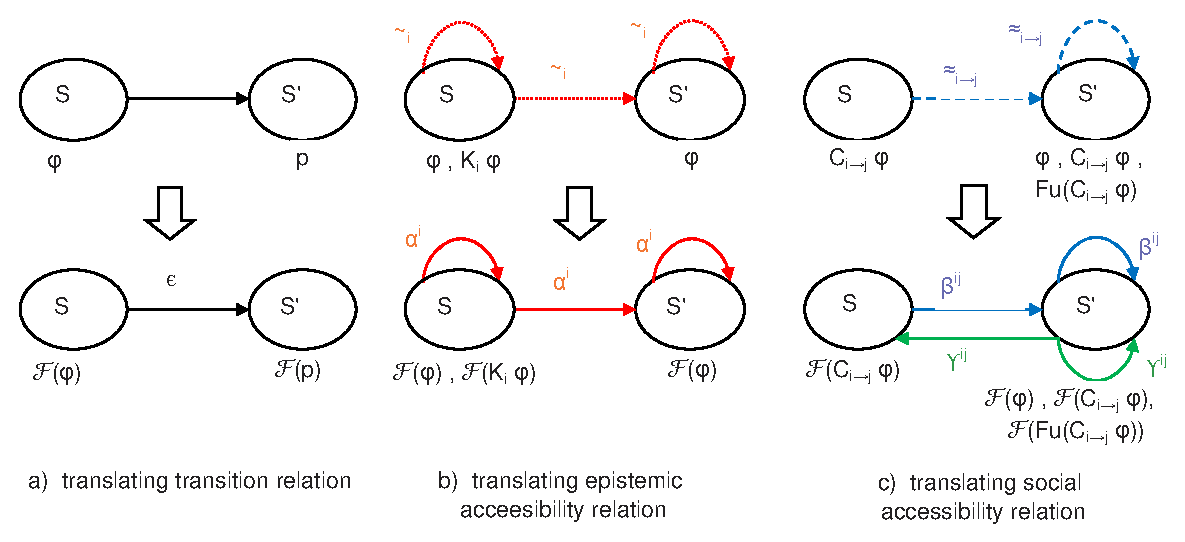
\includegraphics[width=15cm, height=9cm]{chap5/img/relation-translation-cha5.eps}
%height=8cm]{figures/1.eps}
\caption{Examples of translating relations in $\mathfrak{M_3}$ into labeled transitions} \label{fig:relation-translation-cha5}
\end{figure}

%%%%%%%%%%%%%%%%%%%%%%%%%%%%%%%%%%%%%%%%%%%%%%%%%%%%%%%%%%%%%%%%%%%%%%%%%%%%%%

\subsection{Transforming the Model $\mathfrak{M_3}$} \label{sec:reducing-proposed-model-cha5}

As done in Chapter \ref{cha:PCTLKC}, given an MDP model $\mathfrak{M_3'}$ = $(\mathbb{S}, Act, \textsf{P}_t ,I_i, L)$, a major step in transforming $\mathfrak{M_3}$ into $\mathfrak{M_3'}$ is to define the set of actions $Act$. The idea is to map each relation in $\mathfrak{M_3}$ into a corresponding action in $Act$; more specifically, to translate each relation in $\mathfrak{M_3}$ into a labeled transition in $\mathfrak{M_3'}$. Then, these labels (also called actions) are used to form the set $Act$ in $\mathfrak{M_3'}$. Consequently, the different relations in $\mathfrak{M_3}$ namely, probabilistic transition relations, epistemic accessibility relations, and social accessibility relations, are translated into labeled transitions in $\mathfrak{M_3'}$. Moreover, to interpret the fulfillment of a commitment, we need to add the symmetric closure of the transition resulted from translating the social accessibility relation. Figure \ref{fig:relation-translation-cha5} (where $n$ is the number of agents, $1 \leq i \leq n$, and $1 \leq j \leq n$) explains the process of translating the probabilistic transition relation $\textbf{P}$, epistemic accessibility relations $\sim_i$, and social accessibility relations $\approx_{i \to j}$ into labeled transitions. More precisely, the action $\epsilon$ denotes a transition defined from the probabilistic transition relation $\textbf{P}$, action $\alpha^i$ denotes a transition defined from the epistemic accessibility relation $\sim_i$, action $\beta^{ij}$ denotes a transition defined from the social accessibility relation $\approx_{i \rightarrow j}$, and action $\gamma^{ij}$ denotes a transition added to capture the semantics of the fulfillment of a basic commitment. Likewise, the epistemic accessibility relation $\sim_G^E$, and the social accessibility relation $\approx_{i \rightarrow G}$ are translated in the same way where the action $\alpha_G^E$ denotes a transition defined from the epistemic accessibility relation $\sim_G^E$, action $\beta^{G}$ denotes a transition defined from the social accessibility relation $\approx_{i \rightarrow G}$, and the action $\gamma^{G}$ denotes a transition added to capture the semantics of the fulfillment of a group commitment. Consequently, the model $\mathfrak{M_3'} = (\mathbb{S}, Act, \textsf{P}_t ,I_i, L)$ can now be defined as follows:


\begin{itemize}
\item $\mathbb{S}$=$S$; $I_i$=$I$; $L$=$\nu$.

\item $Act = \{\epsilon \} \cup \{\alpha^1, \alpha^2, \dots, \alpha^n, \alpha_G^E\} \cup \{\beta^{11}, \beta^{12}, \dots, \beta^{nn}, \beta^{G}\} \cup \{\gamma^{11}, \gamma^{12}, \dots, \gamma^{nn}, \gamma^{G}\}$ where $n$ is the number of agents.


\item $\textsf{P}_t$ can be defined as the union of the transitions labeled with $\epsilon$,
 transitions labeled with $\alpha^i$, transitions labeled with $\alpha_G^E$, transitions labeled with $\beta^{ij}$, transitions labeled with $\beta^{G}$, transitions labeled with $\gamma^{ij}$, and transitions labeled with $\gamma^{G}$. The probabilities of transitions labeled with $\epsilon$ are not manipulated but rather inherited from the probabilistic transition function $\textbf{P}$. However, transitions labeled with $\alpha^i$ and emanating from the same state are given equal probabilities which reflect the indistinguishably property of epistemic relations over equivalent states. Thus, the probability of each transition annotated by $\alpha^i$ is equal to the probability of each other transition labeled with $\alpha^i$ emanating from the same state which is calculated by dividing one over the number of transitions labeled with $\alpha^i$. The probabilities of transitions labeled with $\alpha_G^E$, $\beta^{ij}$, $\beta^{G}$, $\gamma^{ij}$, and $\gamma^{G}$ are calculated in the same way. For states $s, s' \in \mathbb{S}$ and  action $\theta \in Act$, the function $\textsf{P}_t$ is defined as follows:
\begin{equation*}
    \textsf{P}_t(s, \theta , s' )=
\begin{cases}
    \textbf{P}(s, s'),          & \textrm{if}  ~~\theta = \epsilon  \\
    \frac{1}{|s\sim_i s'|},     & \textrm{if}  ~~ \theta = \alpha^i\\
    \frac{1}{|s\sim_G^E s'|},     & \textrm{if}  ~~ \theta = \alpha_G^E\\
    \frac{1}{|s\approx_{i \rightarrow j} s'|},   & \textrm{if}  ~~ \theta = \beta^{ij}\\
    \frac{1}{|s\approx_{i \rightarrow G} s'|},   & \textrm{if}  ~~ \theta = \beta^{G}\\
    \frac{1}{|s'\approx_{i \rightarrow j} s|},   & \textrm{if}  ~~ \theta = \gamma^{ij}\\
    \frac{1}{|s'\approx_{i \rightarrow G} s|},   & \textrm{if}  ~~ \theta = \gamma^{G}
    \end{cases}
    \end{equation*}

\end{itemize}

As mentioned earlier, the non-deterministic choices in MDP are
resolved using the adversary by picking one enabled transition at
each state, which induces a DTMC model. Technically speaking, the
adversary is a function from the state set $S$ to the action set
$Act$ such that it chooses in any state $s$ one of the enabled
actions. In particular, we define seven adversaries
($\sigma_\epsilon$, $\sigma_e$, $\sigma_G^E$, $\sigma_c$,
$\sigma_c^G$, $\sigma_f$, $\sigma_f^G$) that are used to define
DTMCs from the obtained MDP model as follows: $\sigma_\epsilon$
captures only the semantics of regular temporal formulae,
$\sigma_e$ captures the semantics of the knowledge formulae,
$\sigma_G^E$ captures the semantics of the operator everyone in
the group knows, $\sigma_c$ captures he semantics of the basic
commitment, $\sigma_c^G$ captures the semantics of group social
commitment, $\sigma_f$ captures the semantics of the fulfillment
of the basic commitment, and $\sigma_f^G$ captures the semantics
of the fulfillment of group commitment. Concretely, we set the
adversary $\sigma_\epsilon$ in such a way that always selects the
transitions labeled by $\epsilon$ at each state in the model. This
results in a DTMC model that captures only probabilistic temporal
transitions inherited from $\textbf{P}$ and ignores all
transitions obtained by translating the various accessibility
relations. The adversary $\sigma_e$ always picks the action
$\alpha^i$ at the state $s$ and then selects the action $\epsilon$
at all following states (i.e., first the transitions resulted from
the accessibility relations $\sim_i$ are considered, and then the
normal transitions), and so on for the other adversaries.

To this end, we introduce our reduction rules that translate each PCTL$^{\textrm{kc+}}$ formula to PCTL formula w.r.t a given adversary.

%%%%%%%%%%%%%%%%%%%%%%%%%%%%%%%%%%%%%%%%%%%%%%%%%%%%%%%%%%%%%%%%%%%%

\subsection{Reducing PCTL$^{\textrm{kc+}}$ Formulae into PCTL Formulae} \label{sec:reducing-pctlkc-to-pctl-cahp5}

The PCTL$^{\textrm{kc+}}$ formulae are reduced inductively into PCTL as follows:

$\mathscr{F}(p)=p$, if $p$ is an atomic proposition,

$\mathscr{F}(\neg \varphi)= \neg \mathscr{F} (\varphi)$,

$\mathscr{F}(\mathbb{P}_{\bowtie k}(\varphi \vee \psi))=\mathbb{P}_{\bowtie k}(\mathscr{F}(\varphi) \vee \mathscr{F}(\psi))$,

$\mathscr{F}(\mathbb{P}_{\bowtie k}\bigcirc \varphi)=\mathbb{P}_{\bowtie k} \bigcirc \mathscr{F}(\varphi)$,

$\mathscr{F}(\mathbb{P}_{\bowtie k}(\varphi~ U ~ \psi))=\mathbb{P}_{\bowtie k} (\mathscr{F}(\varphi) U \mathscr{F}(\psi))$,

$\mathscr{F}(\mathbb{P}_{\bowtie k}(\varphi~ U^{\leq m} ~ \psi))=\mathbb{P}_{\bowtie k} (\mathscr{F}(\varphi) U^{\leq m} \mathscr{F}(\psi))$,

$\mathscr{F}(K_i ~\varphi)= \mathbb{P}_{\geq 1}(\bigcirc \mathscr{F}(\varphi))$,

$\mathscr{F}(\mathbb{P}_{\bowtie k} K_i ~\varphi)= \mathbb{P}_{\bowtie k}(\mathbb{P}_{\geq 1}\bigcirc\mathscr{F}(\varphi))$,

$\mathscr{F}(E_G ~\varphi)= \mathbb{P}_{\geq 1}(\bigcirc \mathscr{F}(\varphi))$,

$\mathscr{F}(\mathbb{P}_{\bowtie k} E_G ~\varphi)= \mathbb{P}_{\bowtie k}(\mathbb{P}_{\geq 1}\bigcirc\mathscr{F}(\varphi))$,

$\mathscr{F}(C_{i\rightarrow j} ~\varphi)= \mathbb{P}_{\geq 1}(\bigcirc \mathscr{F}(\varphi))$,

$\mathscr{F}(\mathbb{P}_{\bowtie k} C_{i\rightarrow j} ~\varphi)= \mathbb{P}_{\bowtie k}(\mathbb{P}_{\geq 1}\bigcirc\mathscr{F}(\varphi))$,

$\mathscr{F}(C_{i\rightarrow G} ~\varphi)= \mathbb{P}_{\geq 1}(\bigcirc \mathscr{F}(\varphi))$,

$\mathscr{F}(\mathbb{P}_{\bowtie k} C_{i\rightarrow G} ~\varphi)= \mathbb{P}_{\bowtie k}(\mathbb{P}_{\geq 1}\bigcirc\mathscr{F}(\varphi))$,

$\mathscr{F}(Fu(C_{i\rightarrow j} ~\varphi))= \mathbb{P}_{\geq 1}(\bigcirc \mathscr{F}(C_{i\rightarrow j} ~\varphi))= \mathbb{P}_{\geq 1}(\bigcirc\mathbb{P}_{\geq 1}(\bigcirc \mathscr{F}(\varphi)))$,

$\mathscr{F}(\mathbb{P}_{\bowtie k} Fu(C_{i\rightarrow j} ~\varphi))= \mathbb{P}_{\bowtie k} (\mathbb{P}_{\geq 1}\bigcirc\mathscr{F}(C_{i\rightarrow j} ~\varphi))= \mathbb{P}_{\bowtie k}(\mathbb{P}_{\geq 1}\bigcirc\mathbb{P}_{\geq 1}(\bigcirc \mathscr{F}(\varphi)))$,

$\mathscr{F}(Fu(C_{i\rightarrow G} ~\varphi))= \mathbb{P}_{\geq 1}(\bigcirc \mathscr{F}(C_{i\rightarrow G} ~\varphi))= \mathbb{P}_{\geq 1}(\bigcirc\mathbb{P}_{\geq 1}(\bigcirc \mathscr{F}(\varphi)))$,

$\mathscr{F}(\mathbb{P}_{\bowtie k} Fu(C_{i\rightarrow G} ~\varphi))= \mathbb{P}_{\bowtie k} (\mathbb{P}_{\geq 1}\bigcirc\mathscr{F}(C_{i\rightarrow G} ~\varphi))= \mathbb{P}_{\bowtie k}(\mathbb{P}_{\geq 1}(\bigcirc\mathbb{P}_{\geq 1}(\bigcirc \mathscr{F}(\varphi))))$.\\

To complete the reduction process, each PCTL formula has to be
interpreted over a DTMC model $\mathcal{D}$ =
$(S,\overline{s},\mathbf{P},L)$. This is achieved by indicating
which adversary is associated with which formula. In the
following, $(\mathfrak{M_3'},s)\models_{\sigma_\epsilon} \varphi$
means that the PCTL formula $\varphi$ holds in the model
$\mathcal{D}$ obtained by applying the adversary $\sigma_\epsilon$
at state $s$. The following theorem is a direct consequence of the
definition of $\mathscr{F}$ and can be easily proved by induction
on the structure of the formula.



%%%%%%%%%%%%%%%%%%%%%%%%%%%%%%%%%%%%%%%%%%%%%%%%%%%%

\begin{theorem}[Transformation Satisfaction]\label{theorem:transf-satisf} \hspace{0.5cm}

Considering the following adversaries: $\sigma_\epsilon$, $\sigma_c$, $\sigma_c^G$, $\sigma_f$, $\sigma_f^G$, $\sigma_e$, and $\sigma_G^E$ (which are DTMCs capturing temporal, commitment, and epistemic formulae in the model $\mathfrak{M_3}$), the following equivalences hold:

$(\mathfrak{M_3},s)\models p ~~~~~~~~~~~~~~~~~~~~~~~~~~\text{iff}~ (\mathfrak{M_3'},s) \models_{\sigma_\epsilon} p$

$(\mathfrak{M_3},s)\models \neg \varphi ~~~~~~~~~~~~~~~~~~~~~~~\text{iff}~ (\mathfrak{M_3'},s)\models_{\sigma_\epsilon} \neg \mathscr{F}(\varphi)$

$(\mathfrak{M_3},s)\models \mathbb{P}_{\bowtie k}(\varphi \vee \psi)
~~~~~~~~\text{iff}~ (\mathfrak{M_3'},s) \models_{\sigma_\epsilon}
\mathbb{P}_{\bowtie k} \mathscr{F}(\varphi) \vee
\mathbb{P}_{\bowtie k} \mathscr{F}(\psi) $

$(\mathfrak{M_3},s)\models \mathbb{P}_{\bowtie k}\bigcirc\varphi ~~~~~~~~~~~~~\text{iff}~ (\mathfrak{M_3'},s) \models_{\sigma_\epsilon} \mathbb{P}_{\bowtie k} \bigcirc \mathscr{F}(\varphi)$

$(\mathfrak{M_3},s)\models\mathbb{P}_{\bowtie k}(\varphi~ U ~ \psi) ~~~~~~~~\text{iff}~ (\mathfrak{M_3'},s) \models_{\sigma_\epsilon} \mathbb{P}_{\bowtie k}(\mathscr{F}(\varphi)~ U ~\mathscr{F}(\psi))$

$(\mathfrak{M_3},s)\models\mathbb{P}_{\bowtie k}(\varphi~ U^{\leq m} ~ \psi) ~~\text{iff}~ (\mathfrak{M_3'},s) \models_{\sigma_\epsilon} \mathbb{P}_{\bowtie k}(\mathscr{F}(\varphi)~ U^{\leq m} ~\mathscr{F}(\psi))$

$(\mathfrak{M_3},s)\models K_i \varphi ~~~~~~~~~~~~~~~~~~~~~\text{iff}~ (\mathfrak{M_3'},s)\models_{\sigma_e} \mathbb{P}_{\geq1}(\bigcirc\mathscr{F}(\varphi))$

$(\mathfrak{M_3},s)\models \mathbb{P}_{\bowtie k}K_i \varphi ~~~~~~~~~~~~~~\text{iff}~ (\mathfrak{M_3'},s) \models_{\sigma_e} \mathbb{P}_{\bowtie k}(\mathbb{P}_{\geq1}(\bigcirc\mathscr{F}(\varphi)))$

$(\mathfrak{M_3},s)\models E_G \varphi ~~~~~~~~~~~~~~~~~~~~\text{iff}~ (\mathfrak{M_3'},s)\models_{\sigma_G^E} \mathbb{P}_{\geq1}(\bigcirc\mathscr{F}(\varphi))$

$(\mathfrak{M_3},s)\models \mathbb{P}_{\bowtie k}E_G \varphi ~~~~~~~~~~~~~\text{iff}~ (\mathfrak{M_3'},s) \models_{\sigma_G^E} \mathbb{P}_{\bowtie k}(\mathbb{P}_{\geq1}(\bigcirc\mathscr{F}(\varphi)))$

$(\mathfrak{M_3},s)\models C_{i \rightarrow j}\varphi ~~~~~~~~~~~~~~~~\text{iff}~ (\mathfrak{M_3'},s)\models_{\sigma_c} \mathbb{P}_{\geq1}(\bigcirc\mathscr{F}(\varphi))$

$(\mathfrak{M_3},s)\models \mathbb{P}_{\bowtie k}C_{i \rightarrow j}\varphi ~~~~~~~~~\text{iff}~ (\mathfrak{M_3'},s) \models_{\sigma_c} \mathbb{P}_{\bowtie k}(\mathbb{P}_{\geq1}(\bigcirc\mathscr{F}(\varphi)))$

$(\mathfrak{M_3},s)\models C_{i \rightarrow G}\varphi ~~~~~~~~~~~~~~~\text{iff}~ (\mathfrak{M_3'},s)\models_{\sigma_c^G} \mathbb{P}_{\geq1}(\bigcirc\mathscr{F}(\varphi))$

$(\mathfrak{M_3},s)\models \mathbb{P}_{\bowtie k}C_{i \rightarrow j}\varphi ~~~~~~~~~\text{iff}~ (\mathfrak{M_3'},s) \models_{\sigma_c^G} \mathbb{P}_{\bowtie k}(\mathbb{P}_{\geq1}(\bigcirc\mathscr{F}(\varphi)))$

$(\mathfrak{M_3},s)\models Fu(C_{i \rightarrow j}\varphi) ~~~~~~~~\text{iff}~ (\mathfrak{M_3'},s) \models_{\sigma_f} \mathbb{P}_{\geq 1}(\bigcirc\mathbb{P}_{\geq 1}(\bigcirc \mathscr{F}(\varphi)))$

$(\mathfrak{M_3},s)\models \mathbb{P}_{\bowtie k}Fu(C_{i \rightarrow j}\varphi) ~\text{iff}~ (\mathfrak{M_3'},s) \models_{\sigma_f} \mathbb{P}_{\bowtie k} (\mathbb{P}_{\geq 1}(\bigcirc\mathbb{P}_{\geq 1}(\bigcirc \mathscr{F}(\varphi))))$

$(\mathfrak{M_3},s)\models Fu(C_{i \rightarrow G}\varphi) ~~~~~~~\text{iff}~ (\mathfrak{M_3'},s) \models_{\sigma_f^G} \mathbb{P}_{\geq 1}(\bigcirc\mathbb{P}_{\geq 1}(\bigcirc \mathscr{F}(\varphi)))$

$(\mathfrak{M_3},s)\models \mathbb{P}_{\bowtie k}Fu(C_{i \rightarrow j}\varphi) ~\text{iff}~ (\mathfrak{M_3'},s) \models_{\sigma_f^G} \mathbb{P}_{\bowtie k} (\mathbb{P}_{\geq 1}(\bigcirc\mathbb{P}_{\geq 1}(\bigcirc \mathscr{F}(\varphi))))$

\end{theorem}


This theorem emphasizes that each translated PCTL$^{\textrm{kc+}}$
formula must be interpreted over an appropriate DTMC. That is, if
the PCTL$^{\textrm{kc+}}$ formula includes only temporal
operators, then the corresponding PCTL formula is interpreted over
the DTMC obtained by only considering the normal transitions
(i.e., $\sigma_\epsilon$). Moreover, if the formula has the form
of $K_i~\varphi$, then the corresponding PCTL formula is
interpreted over the DTMC obtained by considering first the
transitions resulted from translating epistemic accessibility
relations $\sim_i$ and then the normal transitions, which shows
why the $K$ operator is translated into the next operator
$\bigcirc$. The same intuition holds for the other epistemic and
social formulae.


%%%%%%%%%%%%%%%%%%%%%%%%%%%%%%%%%%%%%%%%%%%%%%%%%%%

\begin{theorem} [Soundness and Completeness of
$\mathscr{F}$] \label{soundness-CTLKC+}~\\ Let $\mathfrak{M_3}$ and
$\Phi$ be respectively PCTL$^{\textrm{kc+}}$ model and formula and
let $\mathscr{F}(\mathfrak{M_3})$  and $\mathscr{F}(\Phi)$ be the
corresponding model and formula in PCTL. We have
$\mathfrak{M_3}\models\Phi$ iff $\mathscr{F}(\mathfrak{M_3}) \models
\mathscr{F}(\Phi)$.
\end{theorem}


\begin{proof} %\hspace{0.5cm} \\
To prove the soundness (i.e., the necessary condition) and
completeness (i.e., the sufficient condition) of the proposed
reduction technique, we prove that the following three cases are
sound and complete: $\Phi = K_i \varphi$, $\Phi = C_{i \rightarrow
j} \varphi$ and $\Phi = Fu(C_{i \rightarrow j} \varphi)$. We prove
this by induction on the structure of the formula $\Phi$. The
cases when $\Phi = E_G \varphi$, $\Phi = C_{i \to G} \varphi$, and
$\Phi = Fu(C_{i \to G} \varphi)$ can be proved in a similar way.
The cases of PCTL$^{\textrm{kc+}}$ formulae that are also PCTL
formulae are straightforward.

\begin{itemize}
\item $\Phi = K_i ~\varphi$. We have $(\mathfrak{M_3},s)\models K_i
~\varphi ~\text{iff}~ (\mathfrak{M_3},s') \models \varphi$ for every
$s' \in S ~\textrm{such that}~ s\sim_i s'$. Therefore,
$(\mathfrak{M_3},s)\models K_i ~\varphi ~\text{iff}~
(\mathscr{F}(\mathfrak{M_3}),s) \models \mathscr{F}(K_i~\varphi)$.
We know that $\mathscr{F}(\mathfrak{M_3})= \mathfrak{M_3'}$. Now,
$(\mathfrak{M_3'},s) \models \mathscr{F}(K_i~\varphi)$ iff for every
$s' \in \mathbb{S} ~\textrm{such that}~ (s,\alpha^i,s') \in
\textsf{P}_t$, we have $(\mathfrak{M_3'},s') \models
\mathscr{F}(\varphi)$. However, w.r.t the semantics of $~\sigma_e$
which is a DTMC defined to interpret commitment formulae over
$\mathfrak{M_3'}$, it follows that every infinite path $\pi \in
\Pi^{\sigma_e}(s)$ satisfies that $\pi(1)=s'$ and
$(\sigma_e,\pi(1))\models \mathscr{F}(\varphi)$. Thus,
$(\sigma_e,s)\models \bigcirc\mathscr{F}(\varphi)$ for all $\pi
\in \Pi^{\sigma_e}(s)$. As the path quantifier $A$ is not defined
in PCTL, and we have $\mathbb{P}_{\geq1}$ instead, so we obtain
$(\sigma_e,s)\models
\mathbb{P}_{\geq1}(\bigcirc\mathscr{F}(\varphi))$.

\item $\Phi = C_{i \rightarrow j} \varphi$. We have
$(\mathfrak{M_3},s)\models C_{i\rightarrow j}\varphi ~\text{iff}~
(\mathfrak{M_3},s') \models \varphi$ for every $s' \in S
~\textrm{such that}~ s\approx_{i \rightarrow j}s'$. Consequently,
$(\mathfrak{M_3},s) \models C_{i\rightarrow j} \varphi ~\text{iff}~
(\mathfrak{M_3'},s) \models \mathscr{F}(C_{i\rightarrow j}
\varphi)$. It follows that, $(\mathfrak{M_3},s) \models
\mathscr{F}(C_{i\rightarrow j}\varphi)$ iff for every $s' \in
\mathbb{S} ~\textrm{such that}~ (s,\beta^{ij},s') \in
\textsf{P}_t$, we have $(\mathfrak{M_3'},s') \models
\mathscr{F}(\varphi)$. Now, based on the adversary $~\sigma_c$
which is a DTMC defined to interpret commitment formulae over
$\mathfrak{M_3}$, every infinite path $\pi \in \Pi^{\sigma_c}(s)$
satisfies that $\pi(1)=s'$ and $(\sigma_c,\pi(1))\models
\mathscr{F}(\varphi)$. Thus, $(\sigma_c,s)\models
\bigcirc\mathscr{F}(\varphi)$ for all $\pi \in \Pi^{\sigma_c}(s)$.
As the path quantifier $A$ is not defined in PCTL, and we have
$\mathbb{P}_{\geq1}$ instead, so we obtain $(\sigma_c,s)\models
\mathbb{P}_{\geq1}(\bigcirc\mathscr{F}(\varphi))$.

\item $\Phi = Fu(C_{i \rightarrow j} \varphi)$. We have
$(\mathfrak{M_3},s)\models Fu(C_{i\rightarrow j}\varphi)$ iff there
exists $s'\in S$ such that $s'\approx_{i \rightarrow j}s~
\text{and~}(\mathfrak{M_3},s')\models C_{i \rightarrow j}\varphi$.
Consequently, $(\mathfrak{M_3},s)\models
\mathscr{F}(Fu(C_{i\rightarrow j}\varphi))$ iff there exists $s'
\in \mathbb{S}$ such that $(s,\gamma^{ij},s') \in \textsf{P}_t$
and $(\mathfrak{M_3'},s') \models \mathscr{F}(C_{i \rightarrow
j}\varphi)$. Now, w.r.t the adversary $\sigma_f$ which is a DTMC
defined to interpret fulfillment formulae over $\mathfrak{M_3}$, we
obtain at least one infinite path $\pi \in \Pi^{\sigma_f}(s)$ that
satisfies $\pi(1)=s'$ and $(\sigma_f,\pi(1))\models
\mathscr{F}(C_{i \rightarrow j}\varphi)$. Since $E$ is equivalent
to $\mathbb{P}_{>0}$ and $\mathscr{F}(C_{i \rightarrow j}\varphi)$
is equivalent to
$\mathbb{P}_{\geq1}(\bigcirc\mathscr{F}(\varphi))$, so we obtain
$(\sigma_f,s)\models \mathbb{P}_{>0}(\bigcirc\mathbb{P}_{\geq
1}(\bigcirc \mathscr{F}(\varphi)))$.
\end{itemize}
\end{proof}

%%%%%%%%%%%%%%%%%%%%%%%%%%%%%%%%%%%%%%%%%%%%%%%%%%%%

\section{Implementation}\label{sec:implementation-cha5}

We consider the web-based online shopping system \cite{Gomaa2011}
as a case study to evaluate the effectiveness of our proposed
verification technique.

\subsection{Online Shopping System}\label{sec:Online-s-s}

The online shopping system aims at
providing an online shopping environment for customers. Customers
can request to purchase one or more items from the supplier. By
requesting an item, the customer commits towards the supplier to
pay in order for the request to take place. Once the order is
paid, the supplier confirms the order, and commits to deliver the
requested item and enters a planned shipping date. Finally, when
the order is shipped, the customer is notified. Requested item is
either successfully delivered or refund is issued otherwise.

Because of the uncertainty associated to the underlying infrastructures of both commitments (i.e., the internet through which the payment is made and the transport system through which the delivery of purchased goods is done), there is no guarantee that these commitments are going to be fulfilled. Reasoning about and verifying the commitment to pay and the commitment to deliver have to be tackled with uncertainty in mind so that the degree of fulfilling each commitment can be measured, and so on.

We verify the online shopping system by means of
the reduction-based model check technique proposed in Section
\ref{sec:model-checking-pctlkc+}. Figure \ref{fig:Online-ss}
depicts a model for an interaction scenario between one supplier
and one customer. In every experiment, we enlarge the system by increasing the number of customers only. For simplicity, we assume that all customers perform the same commitment, which is the commitment to pay for the requested item, respectively. We also assume that the supplier commits to all customers (i.e. a group commitment) to deliver the requested
items. This allows us to verify both classes of commitment; basic
social commitments and group social commitments.

\begin{figure}%[H]
                \begin{center}
                \includegraphics[width=14cm, height=10cm]{chap5/img/online-s-s.eps}
                %height=9cm]{figures/test}
                \end{center}
                \caption{A model for the case of one supplier and one customer} \label{fig:Online-ss}
%                \label{Stack}
                \end{figure}



\subsection{System Properties}\label{sec:properties}

Properties that capture the probabilistic behavior of the online
shopping system have been verified using PRISM in various
proposals, for instance \cite{Ouchani2014}. In this section,
special emphasis is given to properties related to the concepts of
knowledge and social commitments. Concretely, we verify some
system's properties such as \textit{Safety}, \textit{Liveness}, and \textit{Reachability} that involve probabilistic
knowledge, probabilistic commitments, and combinations of both.
For the case of social commitments, our verification covers both
basic and group social commitments. All defined properties are
expressed in PCTL$^{\textrm{kc+}}$.

\begin{itemize}
\item \texttt{Safety Property:} Verifying formulae expressing this property in the system models ensures avoiding the appearance of bad situations in the real systems. One bad situation that need to be verified is when the (Cus) fulfills his commitment to pay for the requested order but the (Sup) does not commit to deliver the requested item. This situation can be expressed in PCTL$^{\textrm{kc+}}$ as follows: \\
$\varphi_2= \mathbb{P}_{\geq1}\Box\neg[\mathbb{P}_{>0} \Diamond
Fu(C_{cus\to sup} (Pay))\wedge \mathbb{P}_{\geq1}\Box\neg
(C_{sup\to cus} (Deliver))]$

\item \texttt{Liveness Property:} In all computation paths it is always the case that if the customer commits to pay for the requested item, then in the future the customer will eventually make the payment. This can be expressed in PCLT$^{\textrm{kc+}}$ as follows:\\
$\varphi_3= \mathbb{P}_{\geq1}[(C_{cus\to sup} (Pay))\supset \mathbb{P}_{\geq1}\Diamond Fu(C_{cus\to sup} (Pay))]$

\item \texttt{Reachability Property:} One possible example with regard to the online shopping system is that if the customer (Cus) commits towards the supplier (Sup) to pay for the requested item, the state at which the customer can fulfill his commitment should be reached from the initial state. That is, there should be a possibility from the initial state for the customer to reach the fulfilment state. This can be formally expressed in PCLT$^{\textrm{kc+}}$ as follows:\\
$\varphi_1= \mathbb{P}_{>0} \Diamond Fu(C_{cus\to sup} (Pay))$.

\end{itemize}

Furthermore, thanks to the probabilistic model clacking technique,
we can also get the satisfiability of given formulae in terms of
quantitative results. That is, checking whether a given formula
holds in the model with a threshold (at least 0.95\% for example)
is achievable. Let us consider the following examples:

\begin{itemize}
    \item Once the customer fulfills his commitment to pay, he will be aware about the payment with at least 0.95\%.\\
      $\varphi_4 = P_{>0.95}~ Fu (C_{cus\to sup} (Pay)) \supset K_{cus} Pay$

    \item Once the customer fulfills his commitment to pay, the supplier will be aware about the payment  with at least 0.98\%.\\
      $\varphi_5 = P_{>0.98}~ Fu (C_{cus\to sup} (Pay)) \supset K_{sup} Pay$
\end{itemize}

%%%%%%%%%%%%%%%%%%%%%%%%%%%%%%%%%%%%%%%%%%%%%%%%%%%%%%%%%%%%%%%%%%%%%%%%%
%%%%%%%%%%%%%%%%%%%%%%%%%%%%%%%%%%%%%%%%%%%%%%%%%%%%%%%%%%%%%%%%%%%%%%%%%

\subsection{Experimental Results}\label{sec:Experimental-results-cha5}

The online shopping system is encoded into the PRISM input
language as follows. Supplier agent (Sup) and Customer agent (Cus)
are mapped into \emph{modules} in the PRISM language. Each agent's
actions are used to determine the behavior of the agent (i.e., his
local states). For example, Supplier's actions (variables) are:
\textit{Accept}: Accept the request, \textit{Reject}: Reject the
request, \textit{Deliver}: Deliver the requested item,
\textit{Receipt}: Send receipt, \textit{Refund}: Refund in case of
not delivery. The global model is obtained by the synchronization
between all modules (agents).

Our implementation was performed on a TOSHIBA laptop equipped with
32-bit Windows XP with 1 GB of RAM and Genuine Intel(R) CPU at 1.6
GHz. Table \ref{Model-Construction-chap5} reports the results of 15
experiments wherein (Exp.\#) denotes the experiment number,
(\#Agent) denotes the number of agents, (\#States) denotes the
number of reachable states, (\#Transitions) denotes the number of
transitions, and (Construction Time) denotes the time needed for
building the simulated model in seconds. \\

First experiment started with only two agents; One supplier (Sup) and one Customer (Cus). In the rest of experiments, we add one more customer (Cus) each time and report the changes occurring in the size of the model and
the time needed for building the model. These results show that (\#States) and (\#Transitions) grow up exponentially as the system is augmented with more agents. However, the (Construction Time) increases polynomially till we reach a point close to the state
explosion, then it grows up dramatically. Figure
\ref{fig:model-time-cha5} shows the increase in the construction
time as more agents join the system. This dramatic change in the
time needed to build the model reflects the fact that the model
size becomes massive.

%\begin{table}[htp][H]
\begin{table}%[H]
\centering \caption{Verification results of the online shopping
system} \label{Model-Construction-chap5}
\resizebox{\textwidth}{!}{ %
\begin{tabular}{|c|c|l|l|c|}
\hline
\texttt{Exp.\#} &   \texttt{\#Agents}    & \texttt{\#States} & \texttt{\#Transitions} & \texttt{Const. Time (s)}\\
\hline\hline
\texttt{Exp.1}   &2             &30            & 74              &0.031\\
\hline
\texttt{Exp.2}   &3             &210           &700              &0.039\\
\hline
\texttt{Exp.3}   &4             &1470          &6102             &0.047\\
\hline
\texttt{Exp.4}   &5           &$1.02*10^{4}$    &$5.10*10^{4}$   &0.063\\
\hline
\texttt{Exp.5}   &6           &$7.20*10^{4}$    &$4.15*10^{5}$   &0.078\\
\hline
\texttt{Exp.6}   &7           &$5.04*10^{5}$    &$3.31*10^{6}$   &0.109\\
\hline
\texttt{Exp.7}   &8           &$3.52*10^{6}$    &$2.60*10^{7}$   &0.189\\
\hline
\texttt{Exp.8}   &9           &$2.47*10^{7}$    &$2.03*10^{8}$   &0.328\\
\hline
\texttt{Exp.9}   &10          &$1.73*10^{8}$    &$1.56*10^{9}$    &0.516\\
\hline
\texttt{Exp.10}  &11          &$1.21*10^{9}$     &$1.19*10^{10}$   &0.765\\
\hline
\texttt{Exp.11}  &12          &$8.47*10^{9}$    &$9.01*10^{10}$   &1.406\\
\hline
\texttt{Exp.12}  &13          &$5.93*10^{10}$   &$6.79*10^{11}$   &2.219\\
\hline
\texttt{Exp.13}  &14          &$4.15*10^{11}$    &$5.09*10^{12}$  &6.094\\
\hline
\texttt{Exp.14}  &15          &$2.91*10^{12}$   &$3.8*10^{13}$    &8.046\\
\hline
\texttt{Exp.15}  &16          &$2.03*10^{13}$  &$2.82*10^{14}$    &13.406\\
\hline
\end{tabular}}
\end{table}



\begin{figure}%[H]
                \begin{center}
                %\includegraphics[width=10cm, height=6cm]{chap5/img/construction-time-cha5.eps}
                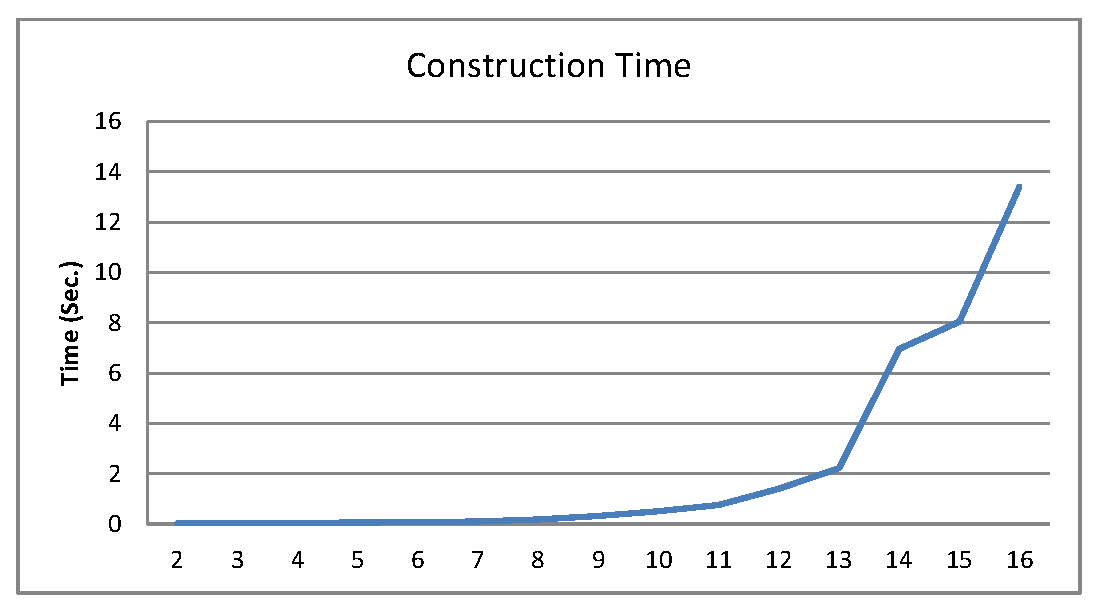
\includegraphics[width=10cm, height=6cm]{chap5/img/time5.eps}
                %height=9cm]{figures/test}
                \end{center}
                \caption{Model construction time for the online shopping system} \label{fig:model-time-cha5}
%                \label{Stack}
                \end{figure}


Table \ref{formulae-prism-results-cha5} reports the model checking
results for the defined formulae ($\varphi_1$ to $\varphi_5$) for
the case of two agents (one customer and one supplier). All
formulae hold in the model as expected, which reflects the success
of our proposed model checking technique in verifying the system
properties expressed using the probabilistic logic
PCTL$^{\textrm{kc+}}$. Moreover, as shown in Table
\ref{formulae-prism-results-cha5}, although the model checking
time varies from one formula to another, it is still short
compared to the time needed for building the model.

For scalability purposes, starting from experiment \#2, we re-write the above-defined formulae in a parameterized form as follows:


$\varphi_1'= \mathbb{P}_{>0} \Diamond \bigwedge\limits_{i=1}^n Fu(C_{cus_i\to sup} (Pay_i))$.

$\varphi_2'= \mathbb{P}_{\geq1}\Box\neg[\mathbb{P}_{>0} \Diamond \bigwedge\limits_{i=1}^n
Fu(C_{cus_i\to sup} (Pay_i))\wedge \mathbb{P}_{\geq1}\Box\neg
(C_{sup\to cus_i} (Deliver_i))]$

$\varphi_3'= \mathbb{P}_{\geq1}[\bigwedge\limits_{i=1}^n (C_{cus_i\to sup} (Pay_i))\supset \mathbb{P}_{\geq1}\Diamond Fu(C_{cus_i\to sup} (Pay_i))]$

$\varphi_4' = P_{>0.95}~ \bigwedge\limits_{i=1}^n Fu (C_{cus_i\to sup} (Pay_i)) \supset K_{cus_i} Pay_i$

$\varphi_5' = P_{>0.98}~ \bigwedge\limits_{i=1}^n Fu (C_{cus_i\to sup} (Pay_i)) \supset K_{sup}
Pay_i$\\
%
where $n$ is the number of agents in the experiment.

\begin{table}%[H]
\centering \caption{Results of model checking some properties for the online shopping system} \label{formulae-prism-results-cha5}
\begin{tabular}{|c|c|c|}
\hline
\texttt{Formulae} &   \texttt{Results}    & \texttt{Time for MC (Sec.)} \\
\hline\hline
$\varphi_1$                &true           &0.06  \\
\hline
$\varphi_2$                &true           &0.13  \\
\hline
$\varphi_3$                &true           &0.11  \\
\hline
$\varphi_4$                &true           &0.06  \\
\hline
$\varphi_5$                &true           &0.07  \\
\hline
\end{tabular}
\end{table}


To be able to verify group social commitments, which is one of the
main motivations of this chapter, we need models of one supplier
agent interacting with two or more customer agents by means of
social commitments. Table \ref{formulae-prism-group-comm-cha5}
reports the results of verifying group social commitments for
experiment \#2 and experiment \#3 using the proposed
reduction technique. In experiment \#2, we have one supplier (Sup) committing to two customers (Cus$_1$) and (Cus$_2$) to deliver the goods. The commitment should be fulfilled in the future to meet the liveness property. Likewise, in experiment \#3, we have one supplier (Sup) committing to three customers (Cus$_1$), (Cus$_2$), and (Cus$_3$) to deliver the requested items.

\noindent $\varphi_6= \mathbb{P}_{\geq1}[(C_{sup \to \{cus_1,cus_2\}} (Deliver))\supset \mathbb{P}_{\geq1}\Diamond Fu(C_{sup \to \{cus_1,cus_2\}} (Deliver))]$

\noindent $\varphi_7= \mathbb{P}_{\geq1}[(C_{sup \to \{cus_1,cus_2,cus_3\}} (Deliver))\supset \mathbb{P}_{\geq1}\Diamond Fu(C_{sup \to \{cus_1,cus_2,cus_3\}} (Deliver))]$

\noindent We were also successful in verifying formulae expressing the interaction between knowledge and group social commitments for experiment \#2 and experiment \#3 as shown below.

\noindent $\varphi_8 = \mathbb{P}_{\geq1}[Fu (C_{sup \to \{cus_1,cus_2\}} (Deliver)) \supset K_{cus_1} (Deliver) \wedge  K_{cus_2} (Deliver)$]

\noindent $\varphi_9 = \mathbb{P}_{\geq1}[Fu (C_{sup \to \{cus_1,cus_2,cus_3\}} (Deliver)) \supset K_{cus_1} (Deliver) \wedge  K_{cus_2} (Deliver) \wedge  K_{cus_3} (Deliver)$]\\

Where, $\varphi_8$ states that the fulfilment of a group commitment (the commitment from $sup$ to $cus_1$ and $cus_2$ to deliver) implies that every creditor in the group will know about the content of the commitment (i.e., $cus_1$ and $cus_2$ will know about the delivery). Similarly, $\varphi_9$ states the same meaning in the case when $sup$ fulfills its commitment to three customers.

\begin{table}[htp]
\centering \caption{Model checking group commitment formulae} \label{formulae-prism-group-comm-cha5}
\begin{tabular}{|c|c|c|c|}
\hline
\texttt{Exp.\#}  &\texttt{\#Agents}  &\texttt{Formulae} &\texttt{Results} \\
\hline\hline
Exp.2            & 1 Sup, 2 Cus      &$\varphi_6$           &true  \\
\hline
Exp.3            & 1 Sup, 3 Cus      &$\varphi_7$           &true  \\
\hline
Exp.2            & 1 Sup, 2 Cus      &$\varphi_8$           &true  \\
\hline
Exp.3            & 1 Sup, 3 Cus      &$\varphi_9$           &true  \\
\hline

\end{tabular}
\end{table}

%%%%%%%%%%%%%%%%%%%%%%%%%%%%%%%%%%%%%%%%%%%%%%%%%%%%

\section{Summary}\label{sec:conclusion}

In this chapter, we introduced a formal approach for specifying and
verifying the interactions between basic (individual) and group social commitments and knowledge in probabilistic MASs. The
proposed approach encompasses three main parts. In the first
part, we presented a new probabilistic logic of knowledge and
commitments (PCLT$^{\textrm{kc+}}$). The expressive power of
PCLT$^{\textrm{kc+}}$ outperforms those of existing logics because
of its ability to express and specify not only the concepts of
knowledge and social commitments independently, but also their
interactions in the presence of uncertainty. Also, being enriched
by operators for the group knowledge and group commitments,
PCLT$^{\textrm{kc+}}$ allows handling more complicated commitment
scenarios with respect to the number of participating agents. We
categorized social commitments into two classes based on the
number of participating agents; basic social commitment (the
common one-to-one scheme) and group social commitment (one-to-many
scheme). We then presented a formal semantics for the group social
commitment. With such a classification of social commitments, we
gain an insight into different ways to utilize commitments among
communicating parties. In contrast, exiting solutions for social commitments restrict themselves to the common one-to-one commitment scheme.

In the second part, we proposed a sound and complete reduction-based model checking technique for the new logic. The proposed technique consists of reducing the problem of model checking PCLT$^{\textrm{kc+}}$ to the problem of model checking PCTL. The soundness and completeness of the reduction technique were proven. Finally, in the third part, we used the
PRISM tool to implement our reduction technique and check
PCLT$^{\textrm{kc+}}$ formulae by checking their corresponding
PCTL formulae without adding new computation cost. In terms of scalability, we showed that our reduction technique is scalable as we were
successfully able to apply it on models of size up to $10^{13}$
states and $10^{14}$ transitions. To conclude, the two main findings of this chapter are:
 \begin{enumerate}
 \item Simply combining a probabilistic logic of knowledge and a probabilistic logic of commitments to capture the interactions between the concept of knowledge and social commitments in probabilistic MASs is not quite working as excepted.
 \item Representing group social commitments and the interactions between group social commitments and knowledge in the presence of uncertainty become attainable by the use of our proposed framework.
 \end{enumerate}



%%%%%%%%%%%%%%%%%%%%%%%%%%%%%%%%%%%%%%%%%%%%%%%%%%%%%%%%%%%%%%%%%%%%%%%%%%%%%%%
%% Chapter 6 : Conclusion.
%%%%%%%%%%%%%%%%%%%%%%%%%%%%%%%%%%%%%%%%%%%%%%%%%%%%%%%%%%%%%%%%%%%%%%%%%%%%%%%
\chapter{Conclusion and Future Work}\label{Chap5:Conclusion}
%********************************************************************
%This chapter concludes the thesis. First, we give a summary of the main contributions of the thesis. Second, we present some hints for future directions.

%********************************************************************
\section{Conclusion}

In this thesis, we have put forward a formal framework for agent communication using a commitment-based approach in order to enable effective agent interactions in open, heterogeneous, and dynamic systems when
uncertainty matters. The main purpose of this framework is to essentially specify and reason about social commitments in probabilistic settings, so they can be formally verified. As an improvement over the existing solutions, our proposed framework targets systems exhibiting probabilistic behavior and considers commitments among a group of agents. The framework is composed of three main components. First, we presented a new probabilistic approach for tackling social commitments in the presence of uncertainty. To specify probabilistic social commitments, we defined a new logic called the probabilistic logic of commitments (PCTLC). Our new logic is interpreted over a new extended version of probabilistic interpreted systems. Furthermore, we introduced a new reduction-based model checking technique for the new logic and implemented it on top of the PRISM model checker. Then, by using the proposed reduction technique, we showed how to evaluate some systems' properties representing probabilistic social commitments -- expressed in terms of the new logic -- against system design models obtained using our extended version of probabilistic interpreted systems.

The second component of our framework focused on the interaction between knowledge and social commitments in probabilistic MASs. We introduced a new logic called the probabilistic logic of knowledge and commitment (PCTL$^{kc}$) to represent and reason about such interactions. PCTL$^{kc}$ logic is interpreted over a new version of probabilistic interpreted systems that has epistemic accessibility relations and social accessability relations at its core. To verify the new logic, we developed a verification technique based on model checking and implemented it using the PRISM tool. Our interest in the first and second contributions was focused on the common two-agent commitment scenarios (i.e. agent-to-agent scheme).

In the third part of the framework, we improved and extended our work in the second part as follows:

\begin{enumerate}

\item We refined and improved PCTL$^{kc}$ to overcome the inconsistency problem appeared when taking the recent work of Al-Saqqar et al. \cite{Al-Saqqar2014a} into consideration. Therefore, in this part, we adopted CTLKC$^+$ \cite{Al-Saqqar2014a} as a basis for our new logic and combined it with PCTL.

\item We extended the scope of interacting agents from agent-to-agent to agent-to-many. This allowed us to investigate different commitment schemes such as the case of committing to multiple agents. In this respect, we defined an adequate semantics for group social commitments for the first time in the literature.
\end{enumerate}

\noindent Based on the new semantics of group social commitments and the consistent logic of knowledge and commitment presented in \cite{Al-Saqqar2014a}, we presented a new probabilistic logic of knowledge and commitment called (PCTL$^{\textrm{kc+}}$). The new logic accommodates new operators for group social commitments and group knowledge in addition to the modalities already found in PCTL$^{kc}$. The expressiveness power of  PCTL$^{\textrm{kc+}}$ outperforms those of existing logics because of its ability not only to capture and express the combinations of knowledge and social commitments in the presence of uncertainty, but also to express formulae involving group social commitments. Formulae of PCTL$^{\textrm{kc+}}$ are interpreted over a new extended version of probabilistic interpreted systems. Our new version of interpreted systems integrates a modified version of social accessabilities that accounts for basic social commitments, group social commitments, and knowledge. To evaluate the new logic (PCTL$^{\textrm{kc+}}$), we proposed a reduction-based model checking technique and implemented it on top of PRISM.

Furthermore, we proved the soundness of all proposed verification techniques. Also, using different case studies we were successfully able to demonstrate the effectiveness and usefulness of our proposed work and evaluate the scalability of the introduced verification techniques.

Finally, as the proposed framework permits addressing probabilistic social commitments as well as their interaction with knowledge when the scope of interacting parties moves beyond the common one-to-one scheme, we believe that it will advance the literature of agent communication and help MASs designers build more effective and efficient systems.

%To conclude, we believe that the proposed framework
%********************************************************************
%* Section 7: Future Work
%********************************************************************
\section{Future Work}

There is

\newpage
\textbf{Publications in refereed journals and conferences}

\textbf{Journals}

\begin{itemize}
\item K. Sultan, J. Bentahar, M. El-Menshawy, "Model Checking Probabilistic Social Commitments for Intelligent Agent Communication", Journal of Applied Soft Computing, Elsevier, 2014.

\item K. Sultan, J. Bentahar, W. Wan, F. Al-Saqqar, "Modeling and Verifying Probabilistic Multi-  Agent Systems using Knowledge and Social Commitments", Journal of Expert Systems with Applications, Elsevier, 2014.

\item F. Al-Saqqar, J. Bentahar, K. Sultan, M. El-Menshawy, "On the Interaction between Knowledge and Social Commitments in Multi-Agent Systems", Applied Intelligence Journal, Springer, 2014.

\item F. Al-Saqqar, J. Bentahar, K. Sultan, W. Wan, E. Khosrowshahi
Asl, "Model Checking Temporal Knowledge and Commitments in Multi-Agent Systems Using Reduction", Simulation Modeling Practice and Theory Journal, Elsevier, 2015.
\end{itemize}

\textbf{Conferences}

\begin{itemize}

\item K. Sultan, J. Bentahar, O. Marey, "A Probabilistic Logic to Reason about the Interaction between Knowledge and Social Commitments in MASs", In the Proc. of The 13th International Conference on Intelligent Software Methodologies, Tools, and Techniques (SOMET\_14), Langkawi, Malaysia, 2014.

\item M. Mbarki, O. Marey, J. Bentahar, K. Sultan,  "Agent Types and Adaptive Negotiation Strategies in Argumentation-Based Negotiation", In the Proc. of the IEEE International Conference on Tools with Artificial Intelligence (ICTAI), Limassol, Cyprus, 2014.

\item K. Sultan, M. El-Menshawy, J. Bentahar, "Reasoning about Social Commitments in the Presence of Uncertainty", In the Proc. of The 12th International Conference on Intelligent Software Methodologies, Tools, and Techniques (SOMET\_13), Budapest, Hungary, 2013.
\end{itemize}

\textbf{Articles in process for publication in refereed journals}

\begin{itemize}
\item K. Sultan, J. Bentahar, R. Mizouni, "Model Checking the Interaction Between Individual and Group Knowledge and Commitments in Probabilistic Multi-Agent Systems", Engineering Applications of Artificial Intelligence, Elsevier, (submitted: August 2014).
\item O. Marey, J. Bentahar, E. Khosrowshahi Asl, K. Sultan, R. Dssouli, "Decision Making under Subjective Uncertainty in Argumentation-Based Negotiation.  Ambient Intelligence and Humanized Computing, (submitted: November 2014).
\end{itemize}




\typeout{------> References}
\bibliographystyle{plain}
\bibliography{ref}
%\appendix
%\input{appendix}


\end{document}


%%% Local Variables:
%%% TeX-master: t
%%% End:
